% \documentclass[embeddedlogo]{ufsc-thesis-rn46-2019}
\documentclass[embeddedlogo,table]{ufsc-thesis-rn46-2019}

\usepackage[T1]{fontenc} % fontes
\usepackage[utf8]{inputenc} % UTF-8
\usepackage{lipsum} % Gerador de texto
\usepackage{pdfpages} % Inclui PDF externo (ficha catalográfica)

% Usado para mostrar código
\usepackage{minted}
\newmintinline[mt]{latex}{fontsize=\normalsize}
\newmintinline[mft]{latex}{fontsize=\footnotesize}
\setminted{fontsize=\tiny,linenos,xleftmargin=2em}
\setmintedinline{breaklines,breakbytokenanywhere}

% Usado para mostrar comandos latex nesse guia:
\newcommand{\lacmd}[1]{\texttt{\textbackslash{}#1}}
\newcommand{\laenv}[1]{\texttt{\textbackslash{}begin\{#1\}...\textbackslash{}end\{#1\}}}
\newcommand{\laenvi}[2]{\texttt{\textbackslash{}begin\{#1\}[#2]...\textbackslash{}end\{#1\}}}

% Pacotes Jeferson Menegazzo
\usepackage{booktabs}
\usepackage{multirow}
%
% \usepackage{pdflscape}
\usepackage{longtable}
% \usepackage{comment}
% \usepackage{float}
% \usepackage{natbib}
% \usepackage{graphicx}
\usepackage{xcolor}

%%%%%%%%%%%%%%%%%%%%%%%%%%%%%%%%%%%%%%%%%%%%%%%%%%%%%%%%%%%%%%%%%%%%
%%% Configurações da classe (dados do trabalho)                  %%%
%%%%%%%%%%%%%%%%%%%%%%%%%%%%%%%%%%%%%%%%%%%%%%%%%%%%%%%%%%%%%%%%%%%%

% Informações para capa e folha de rosto/certificacao

% Caso o título contenha alguma porção LaTeX ilegível, defina um título
% alternativo opcional com []'s para ser usado no campo Title do PDF
% IMPORTANTE: Os títulos deveriam ser iguais. Apenas use um título
% alternativo se o título não puder ser expresso com letras e números
\titulo[Percepção Veicular Adaptativa Baseada em Sensoriamento Inercial e Deep Learning]%
       {Percepção Veicular Adaptativa Baseada em Sensoriamento Inercial e Deep Learning}

\autor{Jeferson Menegazzo}
\data{30 de abril de 2021} % ou \today
\instituicao{Universidade Federal de Santa Catarina}
\centro{Centro Tecnológico}
\local{Florianópolis} % Apenas cidade! Sem estado
\programa{Programa de Pós-Graduação em Ciência da Computação}
% Os dois próximos itens são usados para gerar o \preambulo
\dissertacao % ou \tese ou \tcc
\titulode{mestre em Ciência da Computação}

%%% Atenção! No caso de TCC, além de usar \tcc, outros comandos devem ser fornecidos:
%%%
% \tcc
% \departamento{Departamento de Informática e Estatística}
% \curso{Ciência da Computação}
% \titulode{Bacharel em Ciência da Computação}
% %% Para TCCs, orientadores e coorientadores podem ser externos, logo a
% %% BU exige que sua afiliação seja explicitada. Por padrão, assume-se
% %% UFSC. Você pode alterar a afiliação com os comandos abaixo:
% \afiliacaoorientador{Universidade Federal de Santa Catarina}
% \afiliacaocoorientador{Universidade Federal da Terra de Ninguém}

% Orientador, coorientador, membros da banca e coordenador
% As regras da BU agora exigem que Dr. apareça **depois** do nome
% Dica: para gerar Profᵃ. use Prof\textsuperscript{a}.
% Dica 2: para feminino use \orientadora e \coorientadora
\orientador{Prof. Aldo von Wangenheim, Dr. rer. nat.}
% \coorientador{Prof. Lars Thørväld, Dr.}
% \membrabanca{Prof\textsuperscript{a}. Valerie Béranger, Dr.}{Universidade Federal de Santa Catarina}
\membrobanca{Prof. Fábio Alexandrini, Dr.}{Instituto Federal Catarinense}
\membrobanca{Prof. Alexandre Gonçalves Silva, Dr.}{Universidade Federal de Santa Catarina}
\membrobanca{Prof. Rafael de Santiago, Dr.}{Universidade Federal de Santa Catarina}
% Dica: se feminino, \coordenadora
% \coordenador{Prof. Charles Palmer, Dr}
\coordenadora{Prof. Vania Bogorny, Dr\textsuperscript{a}}


%%%%%%%%%%%%%%%%%%%%%%%%%%%%%%%%%%%%%%%%%%%%%%%%%%%%%%%%%%%%%%%%%%%%
%%% Elementos pré-textuais                                       %%%
%%%%%%%%%%%%%%%%%%%%%%%%%%%%%%%%%%%%%%%%%%%%%%%%%%%%%%%%%%%%%%%%%%%%

\begin{document}

% Inicia parte pré-textual do documento capa, folha de rosto, folha de
% aprovação, aprovação, resumo, lista de tabelas, lista de figuras, etc.
\pretextual%
\imprimircapa%
\imprimirfolhaderosto*
% Atenção! \cleardoublepages são inseridos automaticamente
% Atenção! esse \protect é importante
\protect\incluirfichacatalografica{ficha.pdf}
\imprimirfolhadecertificacao

% Listas de "coisas". O * no final faz com que as listas não sejam 
% incluídas como entratas do sumário (\tableofcontents)

\begin{dedicatoria}
  Este trabalho é dedicado à wikipedia e ao stackoverflow. 
\end{dedicatoria}

\begin{agradecimentos}
  O presente trabalho foi realizado com apoio da Coordenação de Aperfeiçoamento de Pessoal de Nível Superior -- Brasil (CAPES) -- Código de Financiamento 001.
\end{agradecimentos}

\begin{epigrafe}
  For a number of years I have been familiar with the observation that the quality of programmers is a decreasing function of the density of go to statements in the programs they produce \\
  \cite{dijkstra1968}
\end{epigrafe}

%  Aqui deve ser inserido um resumo de 150 a 500 palavras (limitação de tamanho dada pela BU). A linguagem deve ser português e a hifenização já foi alterada. O resumo em português deve preceder o resumo em inglês, mesmo que o trabalho seja escrito em inglês. A BU também diz que deve ser usada a voz ativa e o discurso deve ser na 3ª pessoa. A estrutura do resumo pode ser similar a estrutura usada em artigos: Contexto -- Problema -- Estado da arte -- Solução proposta  -- Resultados.

\begin{resumo}[Resumo]
    Os sistemas de transporte se estabeleceram ao longo da história como um dos principais condicionantes ao desenvolvimento humano. Com o avanço das tecnologias computacionais, surgiram os sistemas de transporte inteligentes, nos quais sensores são empregados na infraestrutura de transporte e seus participantes, de forma a gerar dados brutos que, processados por modelos de IA, geram informações situacionais acerca do modal. Neste contexto, foram desenvolvidas diversas tecnologias de abordagem ativa e passiva. Dentre as tecnologias passivas, existem as baseadas em vibração, realizadas através de sensores inerciais, as quais podem gerar informações situacionais na forma de percepções veiculares, de forma segura, não poluente e de baixo custo. Entretanto, ao contrário de áreas como a visão computacional, o sensoriamento inercial tem sido pouco explorado, onde as soluções propostas no estado-da-arte não são confiáveis para ampla aplicação em cenários do mundo real, uma vez que não são adaptáveis, sendo em sua maioria aplicações simples de prova de conceito. Neste sentido, dado a diversidade contextual na qual a solução pode ser submetida, existem diversos fatores de dependência que interferem e influenciam os valores dos sinais amostrados com estes sensores, de forma que a adaptabilidade da solução a estes fatores se mostra um requisito essencial para prover confiabilidade e, por sua vez, possibilitar uma ampla aplicação. Com este objetivo, neste trabalho propusemos o desenvolvimento de modelos de percepções veiculares baseados em sinais de sensores inerciais, capazes de operar de forma confiável em variações contextuais relacionados aos fatores de dependência: diferentes veículos, estilos de condução e ambientes. Neste trabalho focamos no desenvolvimento das percepções de tipo de superfície de pista, qualidade de superfície de pista, e detecção de lombadas. Para o desenvolvimento e validação dos modelos, coletamos nove conjuntos de dados com variações contextuais, utilizando três veículos diferentes, com três motoristas diferentes, em três ambientes distintos, nos quais existem três tipos de superfície diferentes, além de variações no estado de conservação e a presença de obstáculos e irregularidades. Utilizamos os dados coletados em experimentos para avaliar aspectos como a influência do ponto de coleta de dados do veículo, o domínio de análise, as características de entrada do modelo e a janela de dados. Posteriormente, avaliamos a capacidade de generalização do aprendizado dos modelos para contextos desconhecidos, ou seja, seu comportamento quando aplicado a dados amostrados em um veículo, motorista ou ambiente desconhecido, analisando assim sua adaptabilidade. Os experimentos foram realizados com modelos baseados em aprendizado de máquina clássico e \textit{deep learning}, onde o melhor modelo para classificação de tipo de superfície foi uma rede CNN, a qual classificou segmentos de terra, paralelepípedo e asfalto com acurácia média de 92.70\%; o melhor modelo para classificação de qualidade foi uma rede CNN, a qual classificou segmentos nos níveis bom, regular e ruim com acurácia média de 93.52\%; e o melhor modelo para reconhecimento de lombadas foi uma rede híbrida CNN-LSTM, a qual detectou lombadas com acurácia média de 98.59\%.
    
    % Atenção! a BU exige separação através de ponto (.). Ela recomanda de 3 a 5 keywords
  \vspace{\baselineskip} 
  \textbf{Palavras-chave:} 
  Classificação de Tipo de Superfície de Pista.
  Classificação de Qualidade de Superfície de Pista.
  Detecção de Lombadas.
  Sensores Inerciais. 
  Aprendizado Profundo.
  
\end{resumo}


%\begin{resumo}[Resumo Estendido]
%   \section*{Introdução} 
%   A hifenização é alterada para \texttt{brazil}, mesmo para documentos em inglês. Descrever brevemente esses itens exigidos pela BU. Como a RN 95/CUn/2017 é mais recente e impõe outras regras a revelia de regimentos e regulamentos, é mais sábio obedecê-la. Lembre que esse resumo estendido deve term entre 2 e 5 páginas.
  
%   \lipsum[1]
%   \section*{Objetivos} 
%   \lipsum[2]
%   \section*{Metodologia} 
%   \lipsum[3]
%   \section*{Resultados e Discussão} 
%   \lipsum[4]
%   \section*{Considerações Finais} 
%   \lipsum[5]

%   \vspace{\baselineskip}  % Atenção! manter igual ao resumo
%   \textbf{Palavras-chave:} Palavra-chave. Outra Palavra-chave composta. Bla.
\end{resumo}

\begin{abstract}
  Enlish version of the plain ``resumo'' above. Done with environment
  \texttt{abstract}. Hyphenization is automatically changed to english.

  \vspace{\baselineskip} 
  \textbf{Keywords:} Keyword. Another Compound Keyword. Bla.
\end{abstract}

\listoffigures* % O * evita que apareça no sumário

\listoftables*

% Lista para ambiente algorithm
% \listofalgorithms*

\begin{siglas}
\item[ADAS] \textit{Advanced Driver-Assistance Systems}
\item[ATIS] \textit{Advanced Traveler Information Systems}
\item[ATMS] \textit{Advanced Traffic Management Systems}
\item[APTMS] \textit{Advanced Public Transport Management Systems}
\item[AVCS] \textit{Advanced Vehicle Control Systems}
\item[CID] \textit{Complexity Invariant Distance}
\item[CNN] \textit{Convolutional Neural Network}
\item[CNN-LSTM] \textit{Convolutional Neural Network Long Short-Term Memory}
\item[ConvLSTM] \textit{Convolutional Long Short-Term Memory}
\item[DTW] \textit{Dynamic Time Warping}
\item[DDDTW] \textit{Derivative Dynamic Time Warping}
\item[DTD] \textit{Derivative Transform Distance}
\item[FFT] \textit{Fast Fourier Transform}
\item[FP] Falsos Positvos
\item[FN] Falsos Negativos
\item[GPS] \textit{Global Positioning System}
\item[GRU] \textit{Gated Recurrent Unit}
\item[GT] \textit{Ground Truth}
\item[HC] \textit{Half-Car}
\item[IA] Inteligência  Artificial
\item[IIR] \textit{Infinite Impulse Response}
\item[IRI] \textit{International Roughness Index}
\item[ITS] \textit{Intelligent Transport Systems}
\item[KMC] \textit{K-Means Clustering}
\item[KNN] \textit{K-Nearest Neighbors}
\item[LCSS] \textit{Longest Common Subsequence Similarity}
\item[LSTM] \textit{Long Short-Term Memory}
\item[MSL] Mapeamento Sistemático da Literatura
\item[OBD-II] \textit{On-Board Diagnostic II}
\item[QC] \textit{Quarter-Car}
\item[RQI] \textit{Riding Quality Index}
\item[RSCI] \textit{Road Surface Condition Index}
\item[RSL] Revisão Sistemática da Literatura
\item[SBC] \textit{Single-Board  Computer}
\item[SOM] \textit{Self Organizing Maps}
\item[SVM] \textit{Support Vector Machines}
\item[VP] Verdadeiros Positivos
\item[VN] Verdadeiros Negativos
\end{siglas}


% \begin{listadesimbolos}
  $\gets$   & Atribuição \\
  $\exists$   & Quantificação existencial \\
  $\rightarrow$   & Implicação \\
  $\wedge$   & E lógico \\
  $\vee$   & Ou lógico \\
  $\neg$   & Negação lógica \\
  $\mapsto$   & Mapeia para \\
  $\sqsubseteq$   & Subclasse (em ontologias) \\
  $\subseteq$   & Subconjunto: $\forall x\;.\; x \in A \rightarrow x \in B$ \\
  $\langle\ldots\rangle$ & Tupla \\
  $\forall$   & Quantificação universal \\
  mmmmm & Nenhum sentido, apenas estou aqui para demonstrar a largura máxima dessas colunas. Ao abrir o ambiente \texttt{listadesimbolos}, pode-se fornecer um argumento opcional indicando a largura da coluna da esquerda (o default é de 5em): \texttt{\textbackslash{}begin\{listadesimbolos\}[2cm] .... \textbackslash{}end\{listadesimbolos\}} \\
  $\alpha$   & Alpha \\
  $\beta$   & Beta \\
  $\gamma$   & Gamma \\
  $\delta$   & Delta \\
  $\epsilon$   & Epsilon \\
  $\zeta$   & Zeta \\
  $\eta$   & Eta \\
  $\theta$   & Theta \\
  $\iota$   & Iota \\
  $\kappa$   & Kappa \\
  $\lambda$   & Lambda \\
  $\mu$   & Mu \\
  $\nu$   & Nu \\
  $\xi$   & Xi \\
  $\pi$   & Pi \\
  $\rho$   & Rho \\
  $\sigma$   & Sigma \\
  $\tau$   & Tau \\
  $\upsilon$   & Upsilon \\
  $\phi$   & Phi \\
  $\bowtie$  & Apertem os cintos, uma quebra de página se aproxima! \\
  $\oslash$   & Não use exclamações em lista de símbolos! \\
  $\varphi$   & Varphi \\
  $\chi$   & Chi \\
  $\psi$   & Psi \\
  $\omega$   & Omega \\

\end{listadesimbolos}

\tableofcontents*%

%%%%%%%%%%%%%%%%%%%%%%%%%%%%%%%%%%%%%%%%%%%%%%%%%%%%%%%%%%%%%%%%%%%%
%%% Corpo do texto                                               %%%
%%%%%%%%%%%%%%%%%%%%%%%%%%%%%%%%%%%%%%%%%%%%%%%%%%%%%%%%%%%%%%%%%%%%
\textual%
\chapter{Introdução}
\label{cap:introducao}

Os sistemas de transporte se estabeleceram ao longo da história como um dos principais condicionantes ao desenvolvimento humano. Em sua utilização, seja para circulação de pessoas ou escoamento de produção, intensifica-se cada vez mais demandas por eficiência, dado seu fator estratégico. Neste contexto, com o avanço das tecnologias computacionais, surgiram os Sistemas de Transporte Inteligentes (\textit{Intelligent Transport Systems} - ITS), os quais constituem soluções tecnológicas desenvolvidas para aprimorar o desempenho e a segurança dos sistemas de transporte \cite{Zhang2011,Aragon2016}. Nestas aplicações, o ambiente de tráfego é monitorado através de sensores empregados na infraestrutura de transporte e seus participantes \cite{Zhang2011,mathew2014a,mathew2014b}. Estes sensores produzem dados brutos que são posteriormente processados por modelos computacionais para gerar informações situacionais acerca do modal \cite{Zhang2011}.

Os dados situacionais produzidos em ITS podem ser classificados de diversas maneiras. Uma delas, a percepção veicular, os sensores são empregados de forma a ser possível produzir exterocepções e propriocepções \cite{menegazzo2020}. A exterocepção busca compreender o ambiente fora do veículo, realizando o reconhecimento de características do caminho no qual trafega. Estas características incluem eventos transientes, sendo anomalias e obstáculos tais como buracos, trincas em malha, lombadas etc.; e persistentes, como tipo de pavimentação, condição de conservação e qualidade da superfície da pista. A propriocepção, por sua vez, objetiva compreender os movimentos veiculares para identificar seu próprio comportamento. Estas identificações também podem ser transientes, como eventos de condução, do tipo troca de pista, frenagem, derrapagem, aquaplanagem, virando à direita ou esquerda; e persistentes, como perfil de comportamento de condução em seguro ou perigoso \cite{menegazzo2018,menegazzo2020}.

As informações situacionais produzidas possuem grande aplicabilidade, com impactos sociais, econômicos e ambientais. No suporte à tomada de decisão humana, dados como qualidade do pavimento, e geolocalização de obstáculos e irregularidades na pista podem ser empregados em sistemas gerenciais para planejamento de rotas no escoamento de produção, uma vez que o inadequado estado de conservação do pavimento produz, em média, elevação de 27,0\% dos custos operacionais \cite{CNT2017}. Estes dados também podem ser utilizados por administradoras da via para planejamento de manutenções e controle de tráfego, ou por usuários em Sistemas Avançados de Assistência ao Motorista (\textit{Advanced Driver-Assistance Systems} - ADAS), melhorando a segurança no trânsito. No suporte à tomada de decisão artificial, além dos dados supracitados, outros como tipo de pavimento e perfil de condução podem ser utilizados em veículos autônomos para auxiliar na coordenação de suas ações.

Para a produção dos dados brutos que, após processados, geram as informações na forma de percepção veicular, tecnologias com diferentes abordagens foram propostas, dentre métodos intrusivos e não-intrusivos \cite{NI2016}, conforme ilustra a \autoref{fig:classificacao_sensores}. Na abordagem intrusiva, os dados brutos são amostrados através de sensores colocados diretamente na superfície de via, requerendo possíveis alterações no pavimento ou no tráfego \cite{mathew2014a}. Já na abordagem não-intrusiva, não são realizadas alterações na infraestrutura da via, com os sensores colocados dentro dos veículos que nela trafegam \cite{mathew2014b}. Os métodos não-intrusivos possuem diversas vantagens em relação aos intrusivos, tais como serem menos onerosos, de fácil instalação, cobrirem uma área de monitoramento muito maior e permitirem, além da inspeção da infraestrutura, o acompanhamento das ações dos participantes através da propriocepção.

\begin{figure}[h]
  \centering
  \caption{Abordagens de sensoriamento em ITS}
  \label{fig:classificacao_sensores}
  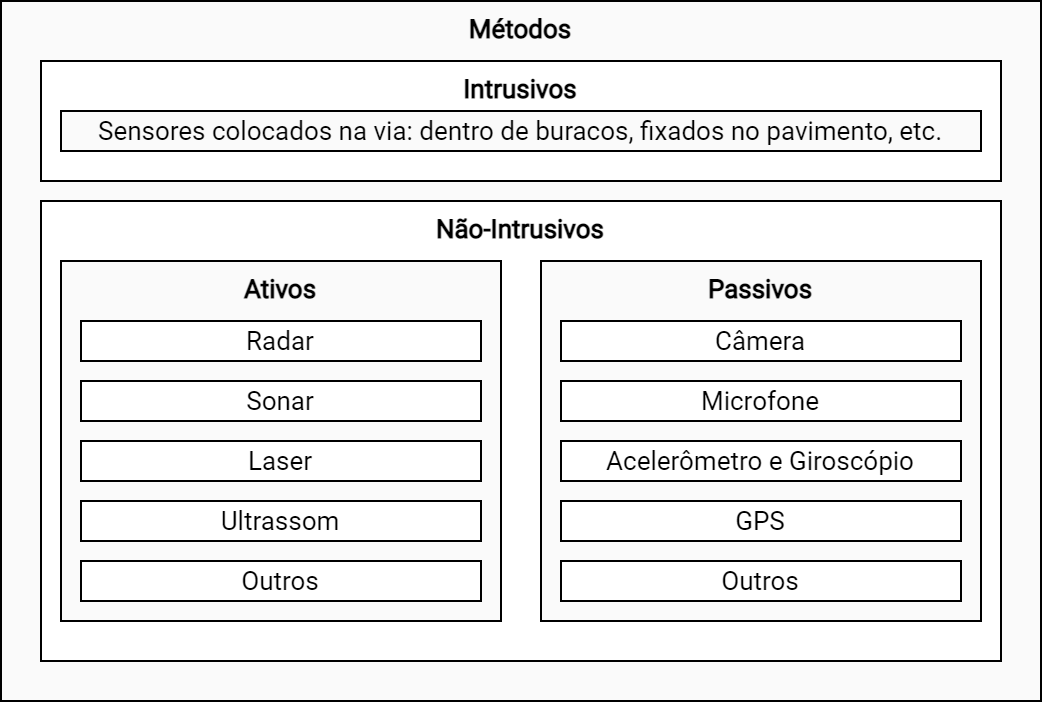
\includegraphics[width=0.9\linewidth]{figuras/fig_1.png}
  \fonte{Desenvolvido pelo autor.}
\end{figure}

Na abordagem não-intrusiva, são empregadas técnicas de sensoriamento passivo e ativo. As técnicas ativas requerem interação com o ambiente para produzir seus dados brutos, com a emissão de ondas no ambiente externo através de laser, ultrassom, sonar ou radar. As técnicas passivas, por sua vez, amostram seus dados sem necessitar interagir com o ambiente externo, como dados físicos ou imagens. Em comparação ao sensoriamento ativo, a abordagem passiva é considerada mais segura, não poluente e geralmente de menor custo. Essas características tornam estas técnicas mais interessantes para uso em larga escala, tal como sua aplicação em sistemas tipo do ADAS ou veículos autônomos. Dentre as soluções de sensoriamento passivo, a utilização de câmeras tem sido amplamente explorada nos últimos anos, com o desenvolvimento de soluções robustas em visão computacional. Contudo, o mesmo não ocorre com os sensores inerciais, representados por acelerômetro e giroscópio, os quais constituem uma alternativa importante a ser melhor explorada \cite{menegazzo2018,menegazzo2020}.

\section{Contextualização do Problema}

Classificados como não-intrusivos e passivos, os sensores inerciais se baseiam no princípio da inércia para produção de seus dados \cite{Braga2017}. Representados por giroscópios e acelerômetros, estes dispositivos produzem, respectivamente, sinais unidimensionais referentes a taxa de rotação e a força de aceleração em seus três eixos físicos \cite{Groves2013}. Neste estudo, estes sinais são resultantes da tração do veículo e das interações com o ambiente no qual ele trafega. Através da aplicação em veículos, sejam fixados diretamente na estrutura veicular ou embarcados em dispositivos móveis como \textit{smartphones} e \textit{tablets}, os sensores inerciais permitem a produção de uma grande diversidade de informações situacionais, conforme ilustra a \autoref{fig:percepcoes_veiculares}.

\begin{figure}[h]
  \centering
  \caption{Percepções veiculares produzidas através de dados de sensores inerciais}
  \label{fig:percepcoes_veiculares}
  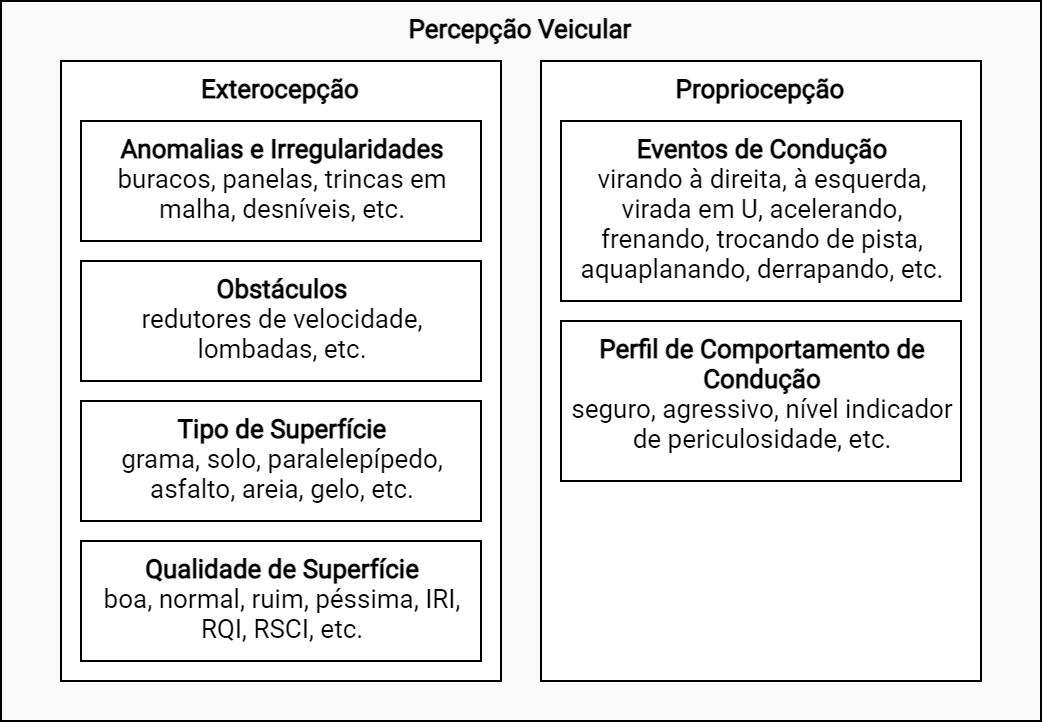
\includegraphics[width=0.9\linewidth]{figuras/fig_2.png}
  \fonte{Desenvolvido pelo autor.}
\end{figure}

Embora sejam diversas e relevantes as percepções veiculares produzidas, a utilização de sensores inerciais em ITS pouco avançou nos últimos anos. Através da Revisão Sistemática da Literatura (RSL) \cite{menegazzo2018,menegazzo2020}, foi observado que a maioria dos estudos da área apresenta foco na aplicação das percepções produzidas. Sendo assim, consistem em pesquisas na forma de prova de conceito, onde as soluções apresentadas para produção de percepções veiculares são simplistas e não aplicáveis a cenários do mundo real, devido a inadaptabilidade dos modelos. Contudo, entendemos que a adaptabilidade é um recurso essencial, onde a solução desenvolvida precisa apresentar um certo grau de confiabilidade quando aplicada em cenários não controlados onde há variações contextuais. Em uma análise comparativa, enquanto soluções baseadas em imagens/vídeos se mostram maduras, com análises em variações contextuais tais como avaliação em diferentes dimensões, marcações desbotadas, diferentes condições de iluminação e oclusão por causa de veículos ou pedestres \cite{Srimongkon2017, Patil2020}, o mesmo não ocorre com os modelos baseados em sinais de sensores inerciais. Nas aplicações desenvolvidas com estes sensores, os modelos analisam cenários controlados e limitados, sem considerar variações de condições no contexto que influenciam os sinais amostrados e, portanto, o resultado da solução final \cite{menegazzo2018,menegazzo2020}.

De acordo com \cite{Carlos2019}, nos últimos 10 anos se produziu uma literatura vasta sobre modelos para produzir informações situacionais a partir dos dados de sensores inerciais fixados no veículo ou embarcados nos \textit{smartphones}. Contudo, é necessário em novas pesquisas tornar os modelos mais inteligentes para traçar o perfil das estradas com detalhes reais \cite{Carlos2019}. Esta afirmação também é sustentada pelos resultados obtidos no levantamento do estado da arte \cite{menegazzo2018,menegazzo2020}, onde observa-se que para um modelo de percepção veicular operar de forma segura e confiável em cenários do mundo real, é necessário considerar os fatores de dependência que impactam nos sinais dos sensores inerciais. Estes fatores estão relacionados à diversidade contextual existente, onde o modelo pode ser aplicado a diferentes veículos, motoristas e ambientes. Considerar estes fatores no modelo o torna adaptável a diferentes condições, sendo este um requisito essencial para sua ampla utilização.

\section{Objetivos}

Nesta seção são detalhados o objetivo geral e específicos desta pesquisa.

\subsection{Objetivo Geral}

Este trabalho objetiva desenvolver modelos adaptativos para produção de percepções veiculares com emprego de sinais de sensores inerciais e técnicas de Inteligência Artificial (IA).  Para satisfazer o requisito de adaptabilidade, os modelos devem demonstrar boa capacidade de generalizar seu aprendizado quando submetido a contextos desconhecidos, os quais apresentam variações contextuais relacionadas as suas propriedades de dependência.

\subsection{Objetivos Específicos}

Os objetivos específicos deste trabalho são:

\begin{itemize}

\item Identificar o estado da arte acerca da produção de percepção veicular através de sinais de sensores inerciais;

\item Desenvolver uma infraestrutura e uma metodologia para coleta de dados brutos;

\item Produzir conjuntos de dados com variações contextuais das propriedades de dependência;

\item Desenvolver um modelo para classificação do tipo de superfície de pista, classificando os sinais dos sensores inerciais entre segmentos de terra, paralelepípedo ou asfalto;

\item Desenvolver um modelo para classificação da irregularidade de superfície de pista,  classificando os sinais dos sensores inerciais entre segmentos de qualidade ruim, regular ou boa;

\item Desenvolver um modelo para detecção de lombadas, através de sinais dos sensores inerciais;

\item Validar a adaptabilidade dos modelos através de um \textit{design} experimental, onde cada modelo será avaliado quanto a sua capacidade de generalização de aprendizado para contextos desconhecidos;

\end{itemize}

\section{Justificativa}

Para disseminar a utilização de ITS em suas mais variadas formas, mostra-se necessário tornar estes sistemas cada vez mais inteligentes. Para isto, é necessário dispor de mais fontes de dados, que estes dados sejam confiáveis, e que os dispositivos que os produzem não sejam prejudiciais à saúde humana quando aplicados em massa. Sendo assim, os sensores inerciais constituem uma fonte de dados alternativa, com grande potencial de melhorar as aplicações em ITS. Devido a sua abordagem passiva, se mostra um meio seguro, não poluente e de baixo custo. A segurança de sua aplicação em massa já foi amplamente validada, uma vez que todo \textit{smartphone} e \textit{tablet} possui um conjunto destes dispositivos. Os sinais produzidos pelos sensores permitem a produção de uma grande variedade de percepções veiculares, dentre exterocepções e propriocepções. Contudo, os atuais modelos de percepção veiculares baseados em sensores inerciais não são confiáveis, se mostrando o principal entrave para sua maior adoção.

A não confiabilidade nos modelos atuais se deve essencialmente a falta de adaptabilidade das soluções. Desta forma, os modelos desenvolvidos não mantêm sua efetividade quando aplicados em cenários diferentes do qual foi experimentado. Sendo assim, os estudos no estado da arte não consideram as variações contextuais pelas quais o modelo será submetido, e os fatores de dependência relacionados. Desta forma, o desenvolvimento de um modelo adaptativo de percepção se mostra de grande contribuição, seja aplicada na tomada de decisão humana ou artificial. Constituindo um aplicação meio para outros sistemas, diversas áreas dos ITS podem se beneficiar, como veículos autônomos, Sistemas Avançados de Controle de Veículos (\textit{Advanced Vehicle Control Systems} - AVCS), Sistemas Avançados de Informação ao Viajante (\textit{Advanced Traveler Information Systems} - ATIS), Sistemas Avançados de Gerenciamento de Tráfego (\textit{Advanced Traffic Management Systems} - ATMS), Sistemas Avançados de Gerenciamento de Transporte Público (\textit{Advanced Public Transport Management Systems} - APTMS), ADAS, entre outros \cite{Zhang2011,Singh2015}.

\subsection{Cenários de Aplicação}

Nesta seção são detalhados alguns cenários de aplicação dos modelos propostos.

\begin{description}

\item [Veículos Autônomo:] Um veículo equipado com sensores inerciais e auxiliares de suporte trafega em uma via. A irregularidade longitudinal da pista, correspondente ao conjunto dos desvios da superfície, é processada em relação a um plano de referência. Nesta análise, é estabelecido um índice de qualidade de conservação e identificado o tipo de pavimentação da via. Também são reconhecidos e classificados eventos transientes de percepção de ambiente, como obstáculos na via (lombadas, redutores de velocidade etc.), deficiências da superfície (buracos, solavancos etc.); e de propriocepção, como eventos de condução (virando à direita suave ou bruscamente, virando à esquerda, acelerando, frenando etc.). Disponibilizando estas informações através de uma interface ao agente inteligente que controla o veículo, o índice de qualidade de superfície e o tipo de pavimentação aferido são empregados no controle de velocidade veicular, sendo menor em vias mais irregulares e vice-versa. Esta decisão pode ser monitorada através dos eventos de condução e, se necessário, efetuado ajustes de comando. Os eventos transientes detectados de percepção de ambiente, utilizados na forma de evidências, auxiliam na convalidação de dados obtidos de sensores multimodais, tal qual por intermédio de visão computacional, corroborando hipóteses sobre o contexto no qual está inserido.

\item [Sistema Avançado de Assistência ao Motorista:] Em um sistema de \textit{vehicular crowdsensing} com sensoriamento oportunista, um \textit{crowdsourcer} utiliza um aplicativo de ADAS em seu computador de bordo ou \textit{smartphone}. Com os sensores inerciais anexados ao veículo ou embarcados nos dispositivos móveis, o aplicativo analisa as vibrações recebidas, para estabelecer conceitos qualitativos sobre a irregularidade de superfície e reconhecer eventos transientes, na forma de obstáculos e anomalias. Um servidor central recebe dados de vários \textit{crowdsourcers}, onde aplica-se um aprendizado baseado em reforço. Empregando a confiabilidade inicialmente estabelecida e a quantidade de detecções em diferentes fontes, a aplicação central realiza ajustes periódicos dos valores de confiabilidade dos dados, de forma que falsos positivos tenham progressivamente sua confiabilidade reduzida a zero, assim como algum evento transiente que deixe de existir, especialmente em função das manutenções realizadas na via. Com esse processamento no servidor, os dados atualizados são baixados pelos \textit{crowdsourcers}, de forma que o aplicativo ADAS utiliza-os para auxiliar o motorista, alertando-o sobre a velocidade acima da segura para uma pista com aquela qualidade de superfície, obstáculos e deficiências durante o trajeto.

\item [Sistema de Monitoramento de Infraestrutura de Transporte Terrestre:] Um veículo e\-qui\-pa\-do com sensores inerciais e auxiliares de suporte trafega em uma via. A irregularidade longitudinal da pista, correspondente ao conjunto dos desvios da superfície, é processada em relação a um plano de referência. Nesta análise, é estabelecido um índice de qualidade de conservação e identificado o tipo de pavimentação da via. Também são reconhecidos e classificados eventos transientes de percepção de ambiente, como obstáculos na via (lombadas, redutores de velocidade etc.), deficiências da superfície (buracos, solavancos etc.). Estas informações situacionais são salvas em um servidor remoto, com as respectivas coordenadas geodésicas. Posteriormente, estes dados são utilizados para definir a manutenção das vias, quando e onde deve ocorrer. Estes dados podem integrar relatórios governamentais, tais como o Relatório Gerencial produzido pela Confederação Nacional do Transporte (CNT), de forma a auxiliar direcionamento de investimentos públicos no modal de transporte terrestre.

\end{description}

\section{Contribuições}

Este trabalho apresenta diversas contribuições de aspecto teórico e aplicado. Com a produção de uma ampla revisão sistemática da literatura, foi realizado o levantamento do estado da arte na aplicação de sensores inerciais para produção de percepções veiculares. Através da análise deste levantamento, foram mapeados todos os fatores de dependência existentes no contexto de ITS que influenciam os sinais amostrados através de sensores inerciais. Este mapeamento, até então inexistente, é importante para que se possa desenvolver modelos de percepção veicular mais robustos, com adaptabilidade ao contexto. Junto a estes fatores, foram produzidos mapeamentos de aspectos diversos, que compreendem desde a etapa da coleta de dados, pré-processamento e processamento.

Com o estabelecimento do estado da arte e mapeamento de aspectos importantes nesta área de pesquisa, foi desenvolvida uma metodologia de coleta de dados, a qual compreende desde a criação da rede de sensores, referenciais de coleta e análise, colocação e posicionamento dos sensores na infraestrutura veicular, etc. Através dessa metodologia, foram produzidos nove conjuntos de dados com variações contextuais relacionadas aos fatores de dependência: diferentes veículos, motoristas e ambientes. Baseando-se nos conjuntos de dados, produzimos um \textit{design} experimental compreendendo as etapas de treinamento e validação dos modelos, de forma a ser possível avaliar a eficiência da generalização de aprendizado do modelo quando aplicado a um contexto desconhecido. Por fim, através de técnicas de \textit{Deep Learning} foram desenvolvidos três modelos adaptativos de percepção veicular, de forma que suas camadas de processamento fossem capazes de compreender as relações entre os dados e seus fatores de dependência. O primeiro modelo classifica o tipo de superfície de pista. O segundo, a qualidade da superfície. Por fim, o terceiro identifica lombadas na via.

Este projeto é inteiramente \textit{open-source}, disponibilizado no Github \footnote{https://github.com/Intelligent-Vehicle-Perception/Intelligent-Vehicle-Perception-Based-on-Inertial-Sensing-and-Artificial-Intelligence} \footnote{https://codigos.ufsc.br/lapix/intelligent-vehicle-perception-based-on-inertial-sensing}. Desta forma, os códigos-fonte utilizados na coleta de dados, para manipulação de sensores, amostragem e armazenamento dos sinais; no pré-processamento, com ajustes, combinação de dados, normalização, etc.; no processamento, com a classificação dos padrões; assim como os próprios datasets e modelos desenvolvidos, estão documentados e disponíveis publicamente, permitindo pesquisas futuras executarem, compararem e auditarem os experimentos. Convém mencionar que os conjuntos de dados produzidos são provavelmente os primeiros do tipo a serem disponibilizados publicamente, com coleta em múltiplos pontos e emprego de diversos sensores de abordagem passiva. Adicionalmente, o projeto conta com diversos materiais de divulgação científica, como vídeos dos sinais e modelos operando, e \textit{Jupyter Notebooks} com fundamentação teórica junto do código-fonte dos melhores modelos. Desta forma, estes materiais auxiliam na popularização deste tipo de sensoriamento em ITS, especialmente por atenuar a curva de aprendizado de novos pesquisadores na área.
 
\section{Estrutura do Trabalho}

Esta dissertação está estruturada em onze capítulos. No \autoref{cap:introducao}, é introduzido o problema de pesquisa, contextualização, justificativa, objetivos, contribuições sociais e científicas para a computação. No \autoref{cap:metodologia} é apresentada a metodologia utilizada neste trabalho, dentre os métodos para levantamento do estado da arte, coleta de dados, desenvolvimento e validação dos modelos. No \autoref{cap:fundamentacao} é discorrida a fundamentação teórica necessária para compreensão desta pesquisa. No \autoref{cap:revisao} é detalhada a revisão da literatura produzida e resultados obtidos, especificando as lacunas de pesquisa existentes com enfoque nas três percepções trabalhadas. No \autoref{cap:conjuntos_de_dados} é detalhada a metodologia de coleta de dados, rede de sensores produzida, referenciais adotados, colocação, posicionamento e configuração, além dos nove conjuntos produzidos. Nos Capítulos \ref{cap:classificacao_tipo_superficie_1} a \ref{cap:deteccao_lombadas} é apresentado a metodologia de desenvolvimento e validação, e os resultados obtidos do modelo adaptativo para classificação de superfície, classificação de qualidade e detecção de lombadas, respectivamente. Por fim, no \autoref{cap:materiais_resultantes} são apresentados os materiais resultantes e no \autoref{cap:conclusoes_discussoes} estão as considerações finais e sugestões de trabalhos futuros.

\chapter{Fundamentação Teórica}
\label{cap:fundamentacao}

Nesta seção são detalhados conceitos acerca dos materiais e métodos utilizados na pesquisa. Inicialmente é discorrido sobre o sensoriamento empregado, tipos de sensores, valores aferidos, entre outras características. Posteriormente, é apresentado o modelo matemático \textit{Quarter-Car} (QC), o qual descreve as mecânicas veiculares envolvidas no processo, e sua representação através das variáveis \textit{Golden Car Parameters}. Por fim, é detalhado o modelo computacional de \textit{Deep Learning} a ser utilizado, com o intuito de reconhecer e classificar os padrões de percepção veicular.

\section{Sensoriamento}

Nesta seção, são apresentados os sensores inerciais, os quais constituem fonte principal de dados do estudo. Em seguida, é discorrido sobre o sensor magnetômetro e GPS, uma vez que servem como sensores auxiliares, comumente utilizados em conjunto com os inerciais para prover informações adicionais. 

\subsection{Sensores Inerciais}

Os sensores inerciais constituem dispositivos que produzem sinais através do princípio da inércia \cite{Braga2017}. Estes sensores compreendem acelerômetros e giroscópios, de um ou mais eixos \cite{Beeby2004}. O acelerômetro mede a força de aceleração (em $m/s^2$ ou g = 9.8 $m/s^2$), enquanto que o giroscópio afere a taxa de rotação (em graus/segundo ou radianos/segundo), ambos sem a necessidade de um referencial externo \cite{Groves2013}. Sendo assim, a partir de um quadro de referência ou posição inicial destes sensores, forças externas que atuam sobre eles causam acelerações e mudanças de orientação (rotação) em um ou mais de seus eixos \cite{Kempe2011}. Neste estudo, essas forças são constituídas pela tração do veículo e pelas interações com o ambiente no qual ele trafega.

\subsubsection{Referenciais}

Os sensores inerciais não requerem nenhum referencial externo. Sendo assim, possuem seu próprio referencial, onde o sistema de coordenadas no qual os dados são amostrados é definido em relação a si próprios. No entanto, a análise dos dados com o objetivo de produzir percepção veicular deve ser realizada no referencial do veículo, como mostra a Figura \ref{fig:quadros_referencia}. Para isso, é necessário reorientar os eixos, mapeando os dados brutos de um sistema para outro.

\begin{figure}[h!]
  \centering
  \caption{Referenciais: (a) Referencial do sensor. (b) Referencial do sensor interno a dispositivos móveis. (c) Referencial da Terra. (d) Referencial do veículo.}
   \label{fig:quadros_referencia}
   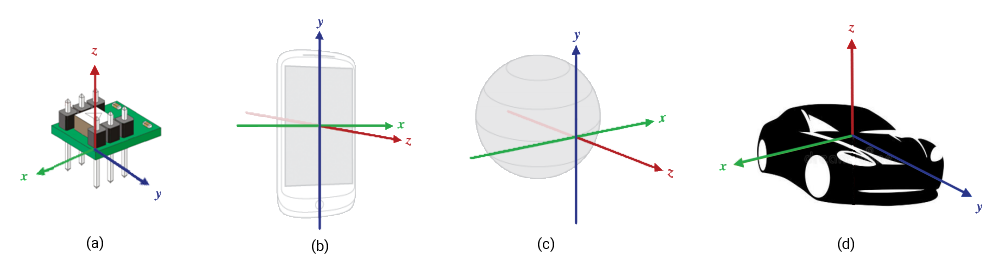
\includegraphics[width=1\textwidth]{figuras/fig2.png}
   \fonte{O autor.}
\end{figure}

A orientação dos dados é importante no processo de análise para que se possa utilizar os valores de acordo com o tipo de percepção a ser realizada. Sendo assim, baseando-se no referencial do veículo, os padrões de percepção de ambiente são mais evidentes na aceleração do eixo Z e na taxa de rotação do eixo Y. Já quanto aos padrões de propriocepção, mostram-se mais evidentes nos dados de aceleração nos eixos X e Y e nas taxas de rotação dos eixos X e Z. Para uma padronização de nomenclatura neste trabalho, serão usados os termos definidos nas Tabelas \ref{table:accelerometer_reference_frames} e \ref{table:gyroscope_reference_frames} para se referir aos dados em relação a cada um dos referenciais.

\begin{table}[h!]
    \caption{Referenciais para os dados de aceleração.}
    \label{table:accelerometer_reference_frames}
    \centering
    \begin{tabular}{clll}
        \toprule
        \textbf{Axis} & \textbf{Sensor} & \textbf{Veículo} & \textbf{Mundo} \\
        \toprule
        X & Aceleração em X & Aceleração Lateral & Aceleração Leste \\
        \midrule
        Y & Aceleração em Y & Aceleração Longitudinal & Aceleração Norte \\
        \midrule
        Z & Aceleração em Z & Aceleração Vertical & Aceleração Vertical (Mundo) \\
        \bottomrule
    \end{tabular}
    \fonte{O autor.}
\end{table}

\begin{table}[h!]
    \caption{Referenciais para os dados de taxa de rotação.}
    \label{table:gyroscope_reference_frames}
    \centering
    \begin{tabular}{clll}
        \toprule
        \textbf{Axis} & \textbf{Sensor} & \textbf{Veículo} & \textbf{Mundo} \\
        \toprule
        X & Taxa de Rotação Pitch & Taxa de Rotação Lateral & N/A \\
        \midrule
        Y & Taxa de Rotação Roll & Taxa de Rotação Longitudinal & N/A \\
        \midrule
        Z & Taxa de Rotação Yaw & Taxa de Rotação Vertical & N/A \\
        \bottomrule
    \end{tabular}
    \fonte{O autor.}
\end{table}

Para a reorientação dos eixos, duas estratégias foram identificadas nos estudos revisados: o posicionamento controlado e o mapeamento através de fórmulas baseadas nos ângulos de Euler. O posicionamento controlado consiste em uma técnica simples, onde sensor é colocado no veículo de forma que os eixos nos referenciais coincidam, ou seja, os eixos do sensor ficam alinhados com os eixos do veículo. Portanto, não é necessário aplicar pré-processamento para reorientação. Essa técnica é usada tanto para os dados do acelerômetro e do giroscópio. 

Os ângulos de Euler, por sua vez, aplicados apenas aos dados de aceleração, fornecem um meio de representar a orientação espacial tridimensional de qualquer referencial como uma composição de três rotações elementares. A orientação de referência pode ser tomada como uma orientação inicial a partir da qual o sistema de coordenadas gira para alcançar sua orientação real \cite{Singh2017}. Assim, essas fórmulas reorientam os dados brutos usando os ângulos fornecidos. Estes dois métodos são detalhados e analisados comparados no Capítulo \ref{cap:revisao}, em conjunto com as demais análises da literatura. 

\subsubsection{Fatores de Dependência}

Os valores amostrados através dos sensores inerciais, embora não dependam de um referencial externo para sua produção, são afetados por propriedades externas e internas aos sensores. Essas propriedades constituem fatores de dependência, que influenciam diretamente a amplitude e dispersão dos valores medidos. Através da tanto da análise da literatura, quando de experimentos exploratórios conduzidos, foi possível observar a existência de fatores de dependência classificados na forma de quatro propriedades, discutidas a abaixo. Para que uma solução desenvolvida possa ser adaptativa na forma que está sendo proposta, é necessário que o modelo considere todas estas propriedades no seu desenvolvimento.

\begin{description}
	
	\item [Propriedades Sensoriais:] 
	
	Quatro fatores de dependência estão relacionados às configurações e características dos sensores, sendo eles a orientação \cite{Kumar2017}, resolução, faixa de medição e taxa de amostragem. A orientação do sensor, conforme discutido na seção anterior, afeta a amostragem de dados no sistema de coordenadas correto. Portanto, o sensor deve ser colocado de forma a ficar alinhado com o sistema de coordenadas do veículo ou ter uma reorientação de eixos para esse referencial. Isso implica na confiabilidade dos dados existentes em cada eixo de análise, pois cada um deles visa atingir certa percepção veicular.

	O segundo e o terceiro fator estão fortemente correlacionados. A resolução é definida de acordo com a faixa de medição escolhida para o sensor. Portanto, é necessário que o sensor tenha uma faixa de medição adequada para poder amostrar os dados sem saturar, ou seja, que a faixa de medição do sensor não seja menor que os valores possíveis a serem monitorados. A resolução, estabelecida a partir da faixa de valores a serem analisados, fornece o quão próximo o valor medido é comparado ao valor real, no processo de quantização. Assim, devido à limitação do número de bits representado pelos sensores, quanto maior a faixa de medição, menor a resolução.
	
	Por fim, a taxa de amostragem descreve a frequência da amostragem de dados por segundo. A escolha desse valor deve levar em consideração não apenas o custo computacional de armazenamento e processamento dos dados amostrados, mas também se, a uma determinada velocidade, será possível obter amostras suficientes para realizar as percepções. Dessa forma, quando o veículo está em alta velocidade, percepções transientes, como buracos, precisam de uma taxa de amostragem satisfatória, para que seja possível adquirir alguma amostra desse evento.
	
	\item [Propriedades Veiculares:] em relação às mecânicas veiculares, o principal fator de dependência é o sistema de suspensão veicular \cite{Kumar2017, Wickramarathne2018}. O sistema de suspensão do veículo, com o objetivo de amortecer os impactos causados pela superfície da pista, faz com que os valores absolutos sejam reduzidos quando medidos acima da suspensão, como ocorre quando os sensores são embarcados em dispositivos móveis. Portanto, os valores amostrados nos sensores anexados no veículo abaixo da suspensão não apresentam essa interferência, embora ainda recebam um pequeno amortecimento causado pelo pneu. Sendo assim, para realizar as percepções em diferentes veículos, deve-se considerar que cada um possui um sistema de suspensão diferente, sendo mais ou menos eficiente.

	\item [Propriedades Ambientais:] estas propriedades não abordadas em trabalhos relacionados, não são tão evidentes, embora necessitem ser consideradas na modelagem da adaptação. Seus fatores de dependência se relacionam com questões climáticas, como superfície de pista com água ou de pouco atrito, que levam a aquaplanagem e derrapagem. Sendo assim, são percepções que implicam na percepção de outras, ou seja, percepções que dependem de percepções. O mesmo ocorre com a variabilidade de superfície, onde a identificação de eventos transientes como buracos e lombadas dependem diretamente do tipo de pavimento que existe na pista, e se existe. Da mesma forma, o dinamismo do estado de conservação de um tipo de pavimento deve ser considerado para detectá-lo corretamente.

	\item [Propriedades de Condução:] as propriedades de condução, intrinsecamente relacionadas as propriedades veiculares, dizem respeito as ações de quem controla o veículo. Nesse sentido, o principal fator de dependência a ser considerado é a velocidade longitudinal \cite{Brunauer2016, Douangphachanh2013, Gueta2017, Kumar2017, Lima2016, M.2017, Nalavde2015, Singh2017}. A velocidade do veículo possui duas implicações. Uma vez que as curvas são feitas em todos os eixos do sistema de coordenadas do veículo, ocorre a produção do componente de força centrífuga. Portanto, as acelerações medidas dependem diretamente da velocidade aplicada. A segunda implicação da velocidade está na distribuição no tempo dos valores amostrados. Em velocidades mais baixas, mais amostras do evento são coletadas e, com o veículo em velocidades diferentes, diferentes quantidades de amostras são obtidas.

\end{description}

\subsection{Magnetômetro}

O magnetômetro é um sensor auxiliar comumente embarcado com os sensores inerciais devido sua função. Este sensor mede o campo geomagnético ambiental (em $\mu$T) em seus três eixos físicos \cite{Sattar2018}. Sendo assim, é geralmente aplicado junto aos ângulos de Euler para dar orientação aos dados e empregado com os dados de aceleração para aproximar dados de localização e velocidade mais rapidamente, uma vez que a taxa de amostragem do GPS é pequena.

\subsection{GPS}

O Sistema de Posicionamento Global (\textit{Global Positioning System} - GPS) consiste de um sistema de satélites que orbitam o planeta, auxiliando receptores em terra a determinar sua localização \cite{Milette2012}. Sendo assim, além dos dados geodésicos de latitude e longitude, o receptor GPS também afere sua velocidade. Embora preciso, este sistema possui uma taxa de amostragem baixa em relação aos demais sensores, cerca de 1Hz.

\section{Quarter Car}

O modelo matemático \textit{Quarter Car} (QC) descreve as variáveis da dinâmica veicular, conforme ilustra a Figura \ref{fig:quarter_car}. O modelo QC possui propriedades relacionadas a roda, suspensão e amortecimento. A propriedade de massa suspensa do veículo (Ms), fica acima da suspensão e representa um quarto da massa veicular. A propriedade de massa não suspensa (Mu), abaixo da suspensão, inclui a massa de uma roda e do sistema de suspensão conectado a ela. Entre as massas, existe a suspensão feita da mola (Ks) e de um amortecedor (C), que suporta a massa suspensa. Uma vez que a massa não suspensa está em contato direto com a superfície da pista, existe a rigidez do pneu (Kt) e a capacidade de absorção do pneu (Ct) impactando nos valores de força \cite{Yafeai2019}.

\begin{figure}[h!]
  \centering
  \caption{O modelo Quarter Car.}
   \label{fig:quarter_car}
   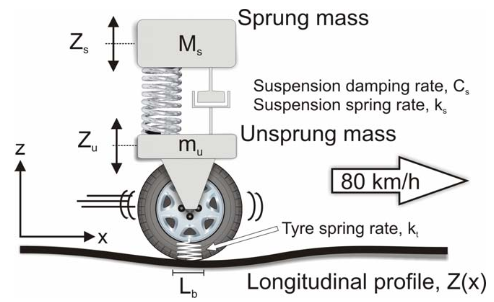
\includegraphics[width=0.6\textwidth]{figuras/fig2_2.png}
   \fonte{\cite{Loizos2008}}
\end{figure}

Através das diversas fórmulas que compõem o modelo, foram criados valores padrões para estas propriedades, denominados \textit{Golden Car Parameters} \cite{Loizos2008}, conforme detalha a Tabela \ref{table:golden_car_parameters}.

\begin{table}[h!]
    \caption{Os parâmetros Golden Car.}
    \label{table:golden_car_parameters}
    \centering
    \begin{tabular}{clll}
        \toprule
        \textbf{Parâmetro} & \textbf{Valor} \\
        \toprule
        Ks/Ms & 63,3 \\
        \midrule
        Kt/Ms & 653 \\
        \midrule
        Cs/Ms & 6 \\
        \midrule
        Mu/Ms & 0,15 \\
        \bottomrule
    \end{tabular}
    \fonte{\cite{Loizos2008}}
\end{table}

\section{Deep Learning}

Com o desenvolvimento do aprendizado de máquina, especialmente a partir de 2006, surgiu nesta área um segmento denominado aprendizado profundo (\textit{Deep Learning}) \cite{Deng2014}. Até então, a extração características importantes que bem representassem os dados parametrizados à uma técnica de reconhecimento de padrões, constituía um problema central. Sendo assim, as técnicas existentes apresentavam a grande dificuldade de se extrair, em um pré-processamento, características de alto nível através de dados brutos \cite{Goodfellow2016}. 

Com o desenvolvimento do \textit{Deep Learning}, esse problema foi solucionado, sendo introduzidas representações que são expressadas em termos de outras, construindo conceitos complexos através de conceitos simples \cite{Goodfellow2016}. Nessa abordagem, tornou-se possível construir modelos computacionais compostos de múltiplas camadas de processamento para aprender a representação dos dados com diversos níveis de abstração \cite{LeCun2015}. Sendo assim, o aprendizado profundo descobre uma estrutura complexa em grandes conjuntos de dados usando o algoritmo de retropropagação para calcular como alterar seus parâmetros internos, os quais são usados para calcular a representação em cada camada a partir da representação na camada anterior \cite{LeCun2015}.

Com este novo paradigma, foram melhorados drasticamente o estado da arte em reconhecimento de fala, reconhecimento visual de objetos, detecção de objetos e muitos outros domínios \cite{LeCun2015}. Os diversos métodos presentes nessa categoria podem ser classificados entre redes profundas para aprendizado não supervisionado ou generativo, redes profundas para aprendizado supervisionado e redes profundas híbridas \cite{Deng2014}. Na categoria de redes profundas para aprendizado supervisionado existem as redes do tipo \textit{Long Short-Term Memory} (LSTM), utilizadas neste trabalho e discorridas na próxima seção.

\subsection{Long Short-Term Memory}

A \textit{Long Short-Term Memory} (LSTM) constitui um tipo de Rede Neural Recorrente (\textit{Recurrent Neural Network} - RNN) considerada ideal para predição e classificação de séries temporais, substituindo muitas abordagens tradicionais por \textit{Deep Learning} \cite{Zaccone2017}. Nesta abordagem, introduzindo o conceito de célula de memória e auto-loops conforme a Figura \ref{fig:cell_lstm}, a rede pode manter valores por um período curto ou longo, como uma função de suas entradas. Assim, a célula consegue se lembrar daquilo que é importante, e não apenas do último valor computado \cite{Jones2017}.

\begin{figure}[h!]
  \centering
  \caption{Célula de memória da LSTM com auto-loop.}
   \label{fig:cell_lstm}
   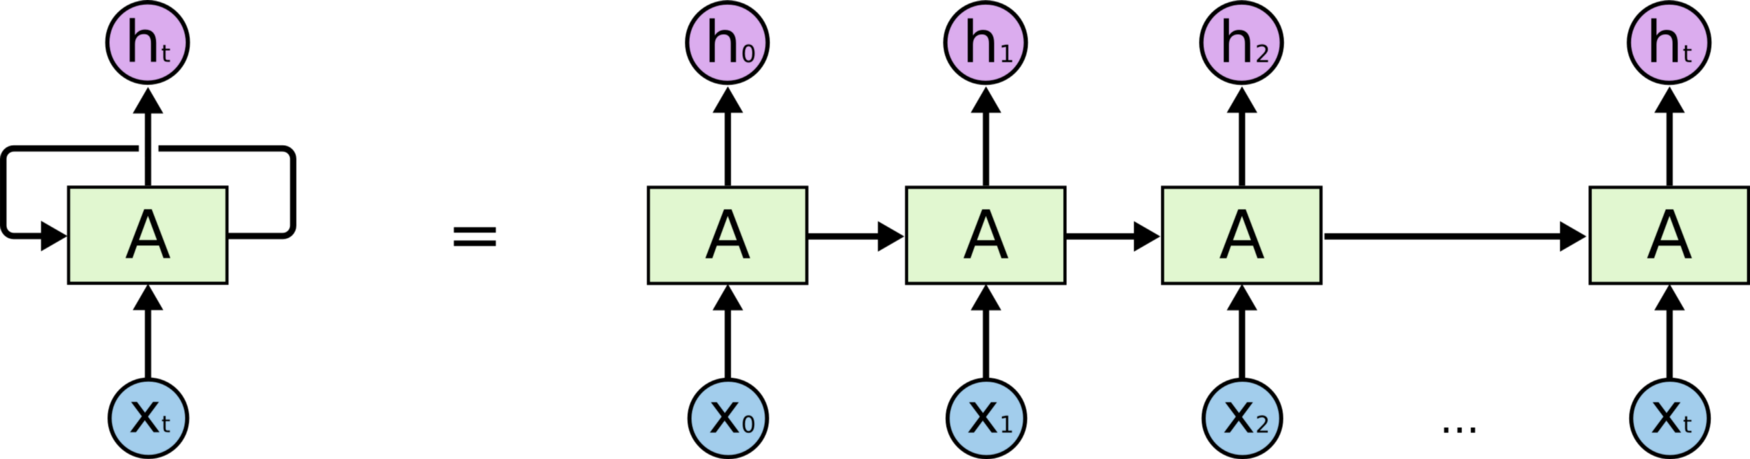
\includegraphics[width=1\textwidth]{figuras/fig2_3.png}
   \fonte{\cite{Junior2019}}
\end{figure}

Cada célula de memória de uma LSTM possuí três portas que controlam o fluxo de informações para dentro e fora da célula. Estas são a porta de entrada (\textit{input gate}), a porta de saída (\textit{output gate}) e a porta de esquecimento (\textit{forget gate}). As portas possuem pesos, onde os valores computados seguem um fluxo no qual resultam em alterações no estado de célula. Sendo assim, inicialmente tem-se a porta de esquecimento, responsável por decidir quais dados devem ser mantidos na memória e quais devem ser esquecidos \cite{Nguyen2018}. Isso permite que a célula se lembre de dados anteriores importantes, ou apenas de novos dados, esquecendo os anteriores. Em seguida, a porta de entrada é responsável por controlar quando novas informações podem entrar na memória. Finalmente, a porta de saída controla quais as informações contidas no próximo estado da célula.\cite{Jones2017}

\begin{figure}[h!]
  \centering
  \caption{Portas da célula de memória da LSTM.}
   \label{fig:cell_lstm_gates}
   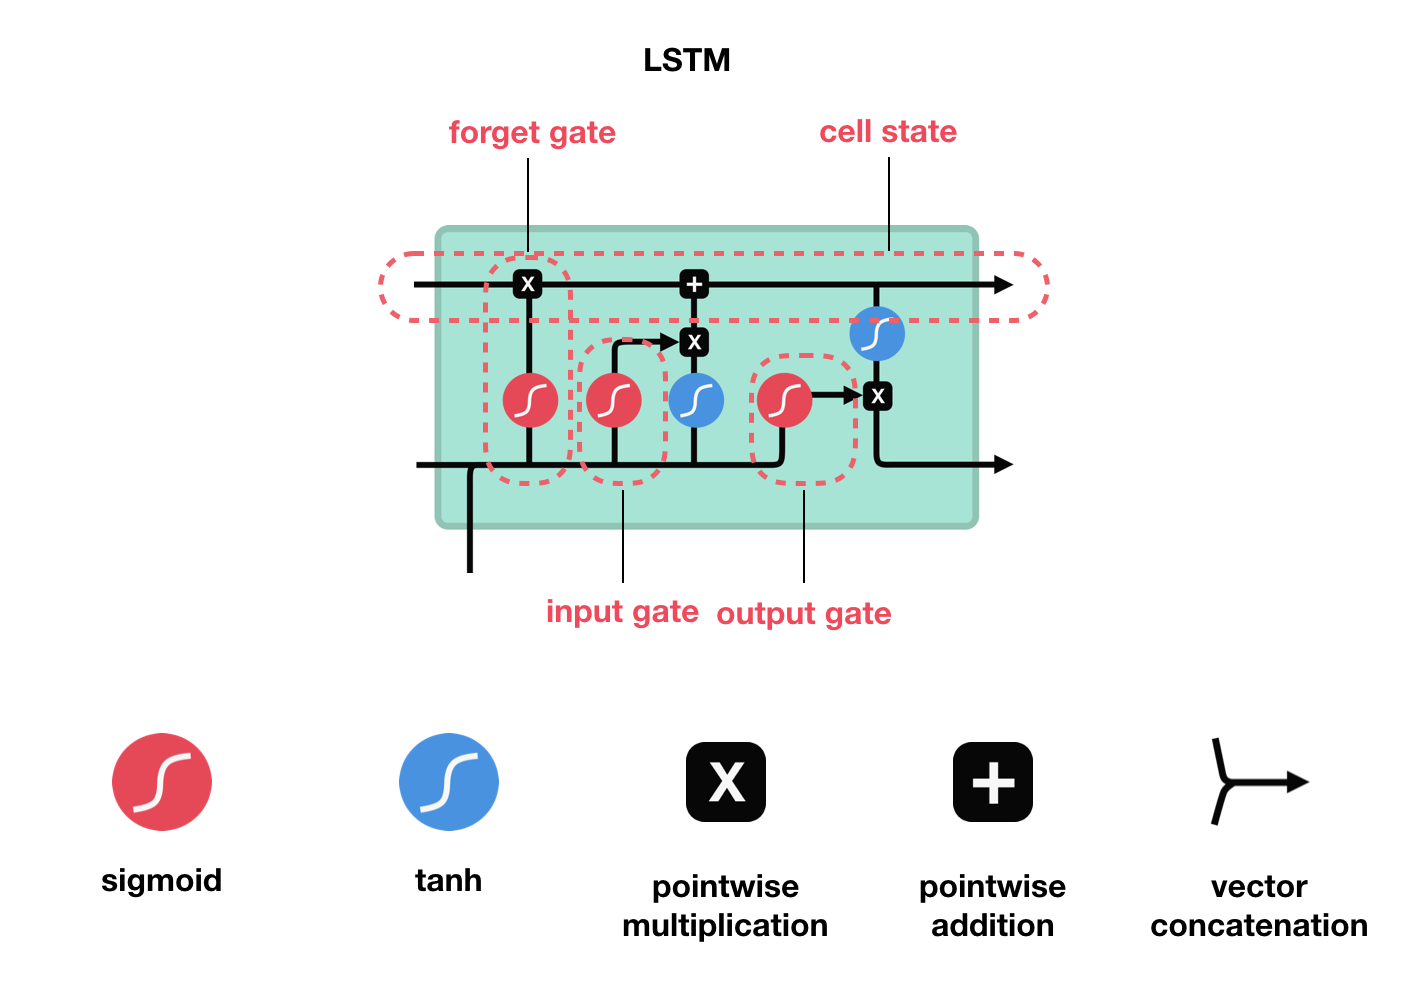
\includegraphics[width=1\textwidth]{figuras/fig2_3_1.png}
   \fonte{\cite{Nguyen2018}}
\end{figure}

\chapter{Fundamentação Teórica}
\label{cap:fundamentacao}

Nesta seção são detalhados conceitos acerca dos materiais e métodos utilizados na pesquisa. Inicialmente é discorrido sobre o sensoriamento empregado, tipos de sensores, valores aferidos, entre outras características. Posteriormente, é apresentado o modelo matemático \textit{Quarter-Car} (QC), o qual descreve as mecânicas veiculares envolvidas no sistema de suspensão. Em seguida, são detalhados as técnicas de IA utilizadas com o intuito de reconhecer e classificar os padrões de percepção veicular, dentre técnicas \textit{Machine Learning} clássico e \textit{Deep Learning}. Por fim, são apresentadas as métricas de avaliação adotadas.

\section{Sensoriamento}

Nesta seção, são apresentados os sensores inerciais, os quais constituem fonte principal de dados do estudo. Em seguida, é discorrido sobre o sensor magnetômetro e GPS, uma vez que servem como sensores auxiliares, comumente utilizados em conjunto com os inerciais para prover informações adicionais. 

\subsection{Sensores Inerciais}

Os sensores inerciais constituem dispositivos que produzem sinais através do princípio da inércia \cite{Braga2017}. Estes sensores compreendem acelerômetros e giroscópios, de um ou mais eixos \cite{Beeby2004}. O acelerômetro mede a força de aceleração (em $m/s^2$ ou g = 9.8 $m/s^2$), enquanto que o giroscópio afere a taxa de rotação (em graus/segundo ou radianos/segundo), ambos sem a necessidade de um referencial externo \cite{Groves2013}. Sendo assim, a partir de um quadro de referência ou posição inicial destes sensores, forças externas que atuam sobre eles causam acelerações e mudanças de orientação (rotação) em um ou mais de seus eixos \cite{Kempe2011}. Em síntese, são sensores que necessitam de movimento para produção de dados. Neste estudo, estes movimentos são resultantes das forças produzidas pela tração do veículo e pelas interações com o ambiente no qual ele trafega.

\subsection{Magnetômetro}

O magnetômetro é um sensor auxiliar comumente embarcado com os sensores inerciais em um mesmo módulo. Este sensor, também de abordagem passiva, mede o campo geomagnético ambiental (em $\mu$T) em seus três eixos físicos \cite{Sattar2018}. Sendo assim, é geralmente aplicado junto aos ângulos de Euler para dar orientação aos dados, reorientando para o referencial da terra. Também é empregado em conjunto com os dados de aceleração para estimar a localização e velocidade mais rapidamente, uma vez que a taxa de amostragem do GPS é muito mais lenta que a dos sensores inerciais.

\subsection{Global Position System}

O Sistema de Posicionamento Global (\textit{Global Positioning System} - GPS) consiste de um sistema de satélites que orbitam o planeta, auxiliando receptores em terra a determinar sua localização \cite{Milette2012}. Sendo assim, além dos dados geodésicos de latitude e longitude, o receptor GPS também afere a velocidade do objeto que contém o sensor. Embora preciso, este sistema possui uma taxa de amostragem baixa em relação aos demais sensores, cerca de 1Hz.

\section{Quarter Car}

O modelo matemático \textit{Quarter Car} (QC) descreve as variáveis da dinâmica veicular, conforme ilustra a \autoref{fig:quarter_car}. O modelo QC possui propriedades relacionadas a roda, suspensão e amortecimento. A propriedade de massa suspensa do veículo $m_s$, fica acima da suspensão e representa um quarto da massa veicular. A propriedade de massa não suspensa $m_u$, abaixo da suspensão, inclui a massa de uma roda e do sistema de suspensão conectado a ela. Entre as massas, existe uma suspensão feita de mola com uma taxa de suspensão $K_s$, e de um amortecedor com uma taxa de amortecimento $C_s$, os quais suportam a massa suspensa. Uma vez que a massa não suspensa está em contato direto com a superfície da pista, existe a rigidez do pneu e sua  capacidade de absorção representadas pela taxa de amortecimento do pneu $K_t$ \cite{Yafeai2019,Loizos2008}. Logo, uma força que parte da superfície da pista atingindo o pneu, será irradiada para todos estes componentes, onde será suavizada pelo deslocamento de massa suspensa $Z_s$ e da massa não suspensa $Z_u$, antes de chegar a parte superior do veículo.

\begin{figure}[h]
  \centering
  \caption{O modelo Quarter Car.}
   \label{fig:quarter_car}
   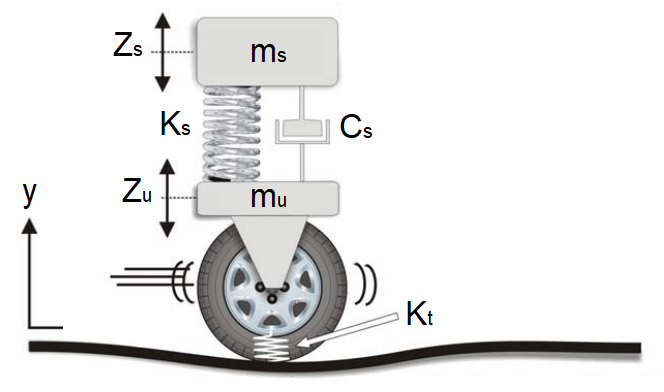
\includegraphics[width=0.8\textwidth]{figuras/fig_4.png}
   \fonte{Adaptado de \cite{Loizos2008}}
\end{figure}

Os valores das variáveis do modelo QC são definidos de acordo com cada veículo, dado as diferentes estruturas veiculares existentes. Este modelo conta com diversas fórmulas que descrevem o relacionamento entre todas as suas variáveis. Os parâmetros do modelo são essenciais na aplicação de metodologias internacionais para indexação da irregularidade, como o IRI, para estabelecer a qualidade da via. De forma a simplificar as fórmulas do QC, foram criados valores padrões para as propriedades, denominados \textit{Golden Car Parameters}. Estas propriedades, detalhadas na \autoref{table:golden_car_parameters}, foram estabelecidas considerando um cenário padrão, onde o veículo é dirigido a uma velocidade constante de 80 $km/h$ \cite{Loizos2008}.

\begin{table}[h]
    \caption{Os parâmetros \textit{Golden Car}}
    \label{table:golden_car_parameters}
    \centering
    \small
    \begin{tabular}{cl}
        \toprule
        \textbf{Parâmetro} & \textbf{Valor} \\
        \toprule
        $K_s/m_s$ & 63,3 \\
        \midrule
        $K_t/m_s$ & 653 \\
        \midrule
        $C_s/m_s$ & 6 \\
        \midrule
        $m_u/m_s$ & 0,15 \\
        \bottomrule
    \end{tabular}
    \fonte{Adaptado de \cite{Loizos2008}}
\end{table}

\section{Técnicas Clássicas de Machine Learning}

Com o desenvolvimento da Inteligência Artificial, diversas técnicas surgiram para resolver problemas de classificação, regressão e previsão. Dentre as técnicas clássicas de \textit{clustering} e aprendizado de máquina supervisionado, neste trabalho foram desenvolvidos modelos de \textit{K-Means Clustering} (KMC), \textit{K-Nearest Neighbors} (KNN) e \textit{Support Vector Machines} (SVM), detalhadas nas próximas subseções.

\subsection{K-Means Clustering}

O KMC consiste de uma técnica não supervisionada para agrupamento de dados (\textit{clustering}), que permite identificar agrupamentos (\textit{clusters}) de dados semelhantes, conforme ilustra a \autoref{fig:execucao_kcm}. Neste método, partindo de um conjunto de dados não rotulados (1), são criadas aleatoriamente centróides para cada um dos \textit{k clusters} (2). Em seguida, cada dado é atribuído a um dos \textit{clusters} baseando-se em uma métrica de distância, como a Euclidiana, em relação à centroide do \textit{cluster} (3, 4). Iterativamente, a centroide de cada \textit{clusters} é recalculada com base na média dos dados (5), e as distâncias novamente recalculadas (6, 7), até que as centróides sejam estabilizadas, ou o número máximo de iterações atingido \cite{foley2019,nisbet2009}.

\begin{figure}[h]
  \centering
  \caption{Execução da técnica KMC.}
   \label{fig:execucao_kcm}
   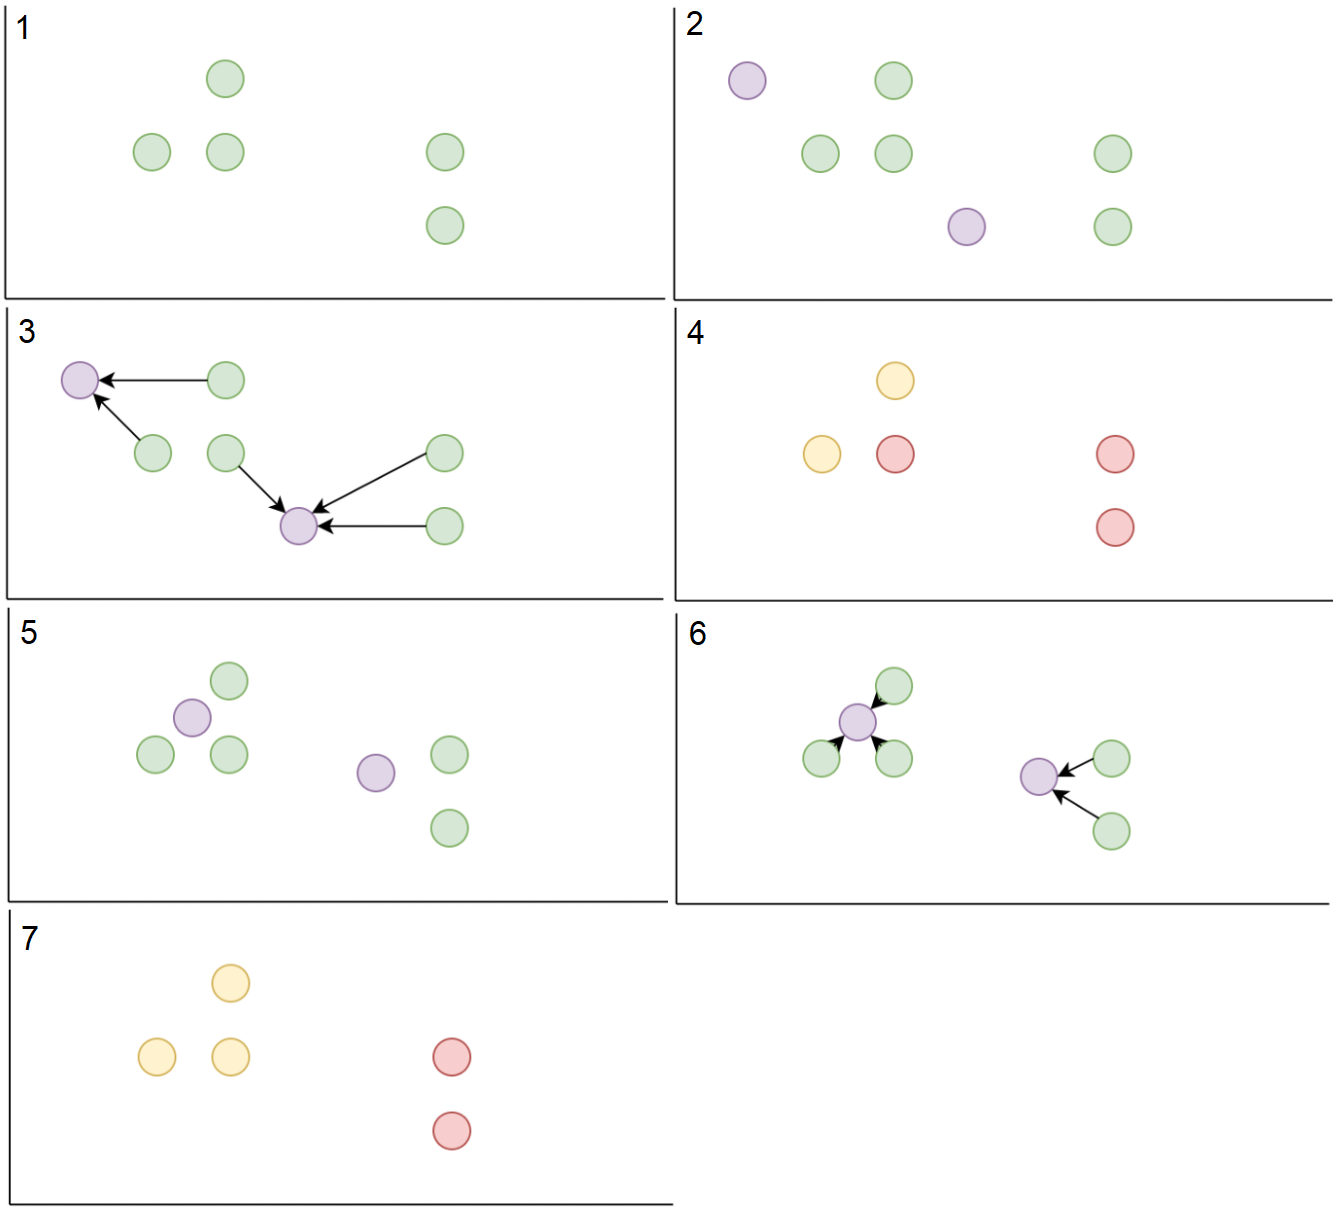
\includegraphics[width=0.7\textwidth]{figuras/fig_5.png}
   \fonte{Adaptado de \cite{i2020}}
\end{figure}

\subsection{K-Nearest Neighbors}

O KNN consiste de uma técnica para classificação a qual se baseia em métricas de similaridades entre os dados para reconhecer padrões. Desta forma, para um novo dado a ser classificado é calculada a distância entre ele e cada um dos dados de treinamento, identificando os k vizinhos mais próximos. A classe do novo dado é definida como aquela mais comum entre seus k vizinhos, conforme ilustra a \autoref{fig:execucao_knn} \cite{Khandelwal2018}.

\begin{figure}[h]
  \centering
  \caption{Execução da técnica KNN.}
   \label{fig:execucao_knn}
   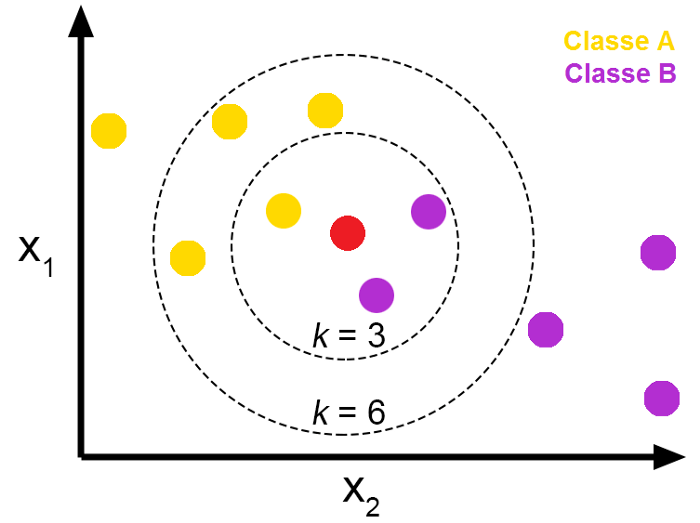
\includegraphics[width=0.4\textwidth]{figuras/fig_6.png}
   \fonte{\cite{Jose2018}}
\end{figure}

\subsection{Support Vector Machines}

O SVM é uma técnica de aprendizado supervisionado aplicada em classificação, onde se busca por um hiperplano ideal que separa as classes de dados, conforme ilustra a \autoref{fig:execucao_svm}. O algoritmo se inicia com a busca pelos pontos mais próximos ao hiperplano que separa as classes. Esses pontos são chamados de vetores de suporte. Na sequencia, é calculada a distância entre o hiperplano e estes vetores. Essa distância é chamada de margem, a qual o SVM busca maximizar, de forma a encontrar o hiperplano ideal \cite{Pupale2019}. Em problemas não lineares, como é o caso deste, é necessário a utilização do hiperparâmetro kernel, o qual converte problema não separável em problema separável, para que o SVM possa classificar \cite{Shubham2018}.

\begin{figure}[h]
  \centering
  \caption{Execução da técnica SVM.}
   \label{fig:execucao_svm}
   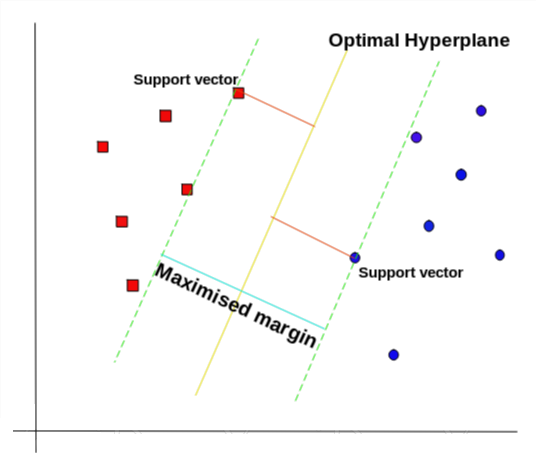
\includegraphics[width=0.7\textwidth]{figuras/fig_7.png}
   \fonte{\cite{Pupale2019}}
\end{figure}

\section{Técnicas de Deep Learning}

Com o desenvolvimento do aprendizado de máquina, especialmente a partir de 2006, surgiu nesta área um segmento denominado aprendizado profundo (\textit{Deep Learning}) \cite{Deng2014}. Até então, a extração características importantes que bem representassem os dados parametrizados à uma técnica de reconhecimento de padrões, constituía um problema central. Sendo assim, as técnicas existentes apresentavam a grande dificuldade de se extrair, em um pré-processamento, características de alto nível através de dados brutos \cite{Goodfellow2016}. 

Com o desenvolvimento do \textit{Deep Learning}, esse problema foi solucionado, sendo introduzidas representações que são expressadas em termos de outras representações, construindo conceitos complexos através de conceitos simples \cite{Goodfellow2016}. Nessa abordagem, tornou-se possível construir modelos computacionais compostos de múltiplas camadas de processamento para aprender a representação dos dados com diversos níveis de abstração \cite{LeCun2015}. Sendo assim, o aprendizado profundo descobre uma estrutura complexa em grandes conjuntos de dados utilizando do algoritmo de retropropagação para calcular como alterar seus parâmetros internos, os quais são usados para estabelecer a representação em cada camada a partir da representação obtida na camada anterior \cite{LeCun2015}.

Com este novo paradigma, foram melhorados drasticamente o estado da arte em reconhecimento de fala, reconhecimento visual de objetos, detecção de objetos e muitos outros domínios \cite{LeCun2015}. Os diversos métodos presentes nessa categoria podem ser classificados entre redes profundas para aprendizado não supervisionado ou generativo, redes profundas para aprendizado supervisionado e redes profundas híbridas \cite{Deng2014}. Neste trabalho, foram utilizadas redes  profundas para aprendizado supervisionado do tipo \textit{Long Short-Term Memory} (LSTM), \textit{Convolutional Long Short-Term Memory} (ConvLSTM), \textit{Gated Recurrent Unit} (GRU)  e \textit{Convolutional Neural Network} (CNN), assim como redes profundas híbridas do tipo \textit{Convolutional Neural Network Long Short-Term Memory} (CNN-LSTM), discorridas nas próximas seções.

\subsection{Long Short-Term Memory}

A LSTM constitui um tipo de Rede Neural Recorrente (\textit{Recurrent Neural Network} - RNN) considerada ideal para predição e classificação de séries temporais, substituindo muitas abordagens tradicionais por \textit{Deep Learning} \cite{Zaccone2017}. Suas aplicações envolvem previsão ou classificação de séries temporais \cite{Zaccone2017}, tais como previsão de velocidade de tráfego, modelagem de linguagem, reconhecimento de fala, aprendizagem de gramática, modelagem de áudio, reconhecimento de caligrafia, etc. \cite{Bianchi2017}. Nesta abordagem, introduzindo o conceito de estado de célula (memória) e \textit{auto-loops} conforme ilustra a \autoref{fig:cell_lstm}, a rede pode manter valores por um curto ou longo período de tempo, como uma função de suas entradas. Assim, a célula consegue se lembrar daquilo que é importante, e não apenas do último valor computado \cite{Jones2017}, de forma que informações relevantes de entradas anteriores são retidas e utilizadas para alterar a saída atual \cite{Zebin2018}.

\begin{figure}[h]
  \centering
  \caption{Célula de uma LSTM com \textit{auto-loop}.}
   \label{fig:cell_lstm}
   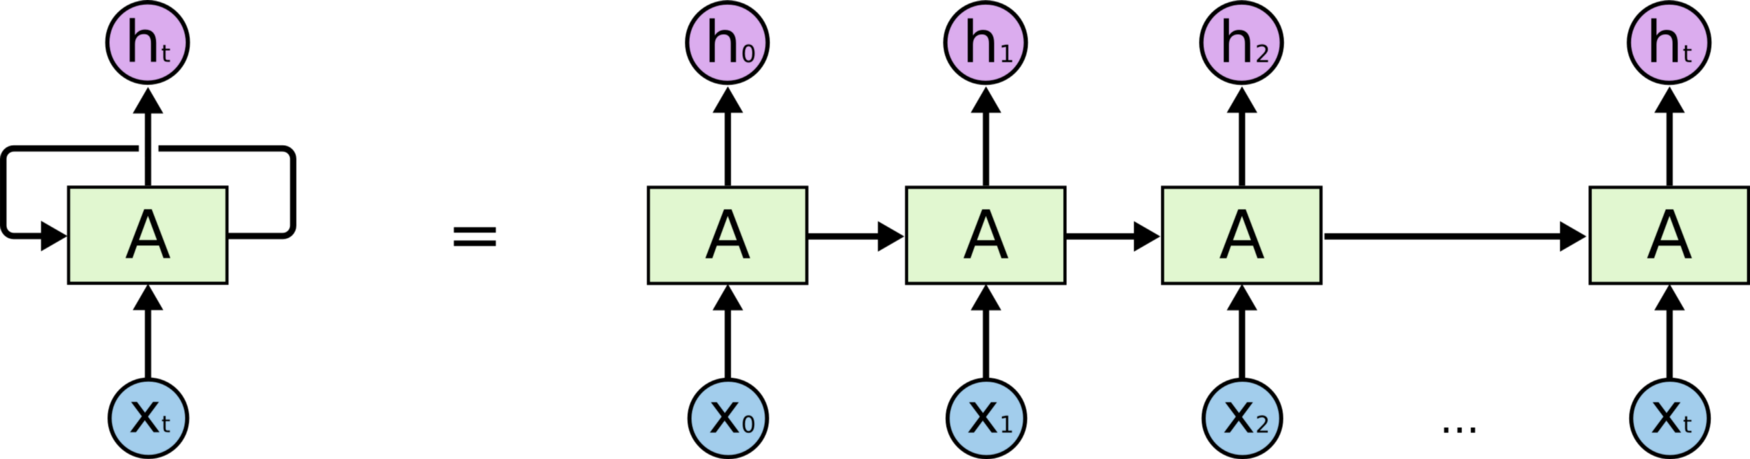
\includegraphics[width=0.8\textwidth]{figuras/fig_8.png}
   \fonte{\cite{Junior2019}}
\end{figure}

Cada célula de uma LSTM possuí três portas que controlam o fluxo de informações para dentro e fora da célula, ilustrado na \autoref{fig:cell_lstm_gates}. Estas são: a porta de entrada (\textit{input gate}), a porta de saída (\textit{output gate}) e a porta de esquecimento (\textit{forget gate}). As portas possuem pesos, onde os valores computados seguem um fluxo no qual resultam em alterações no estado de célula. Sendo assim, inicialmente tem-se a porta de esquecimento, responsável por decidir quais dados devem ser mantidos na memória e quais devem ser esquecidos \cite{Phi2020}. Isso permite que a célula se lembre de dados anteriores importantes, ou apenas de novos dados, esquecendo os anteriores. Em seguida, a porta de entrada é responsável por controlar quando novas informações podem entrar na memória. Finalmente, a porta de saída controla quais as informações contidas no próximo estado da célula \cite{Jones2017}.

\begin{figure}[h]
  \centering
  \caption{Componentes de uma célula de LSTM.}
   \label{fig:cell_lstm_gates}
   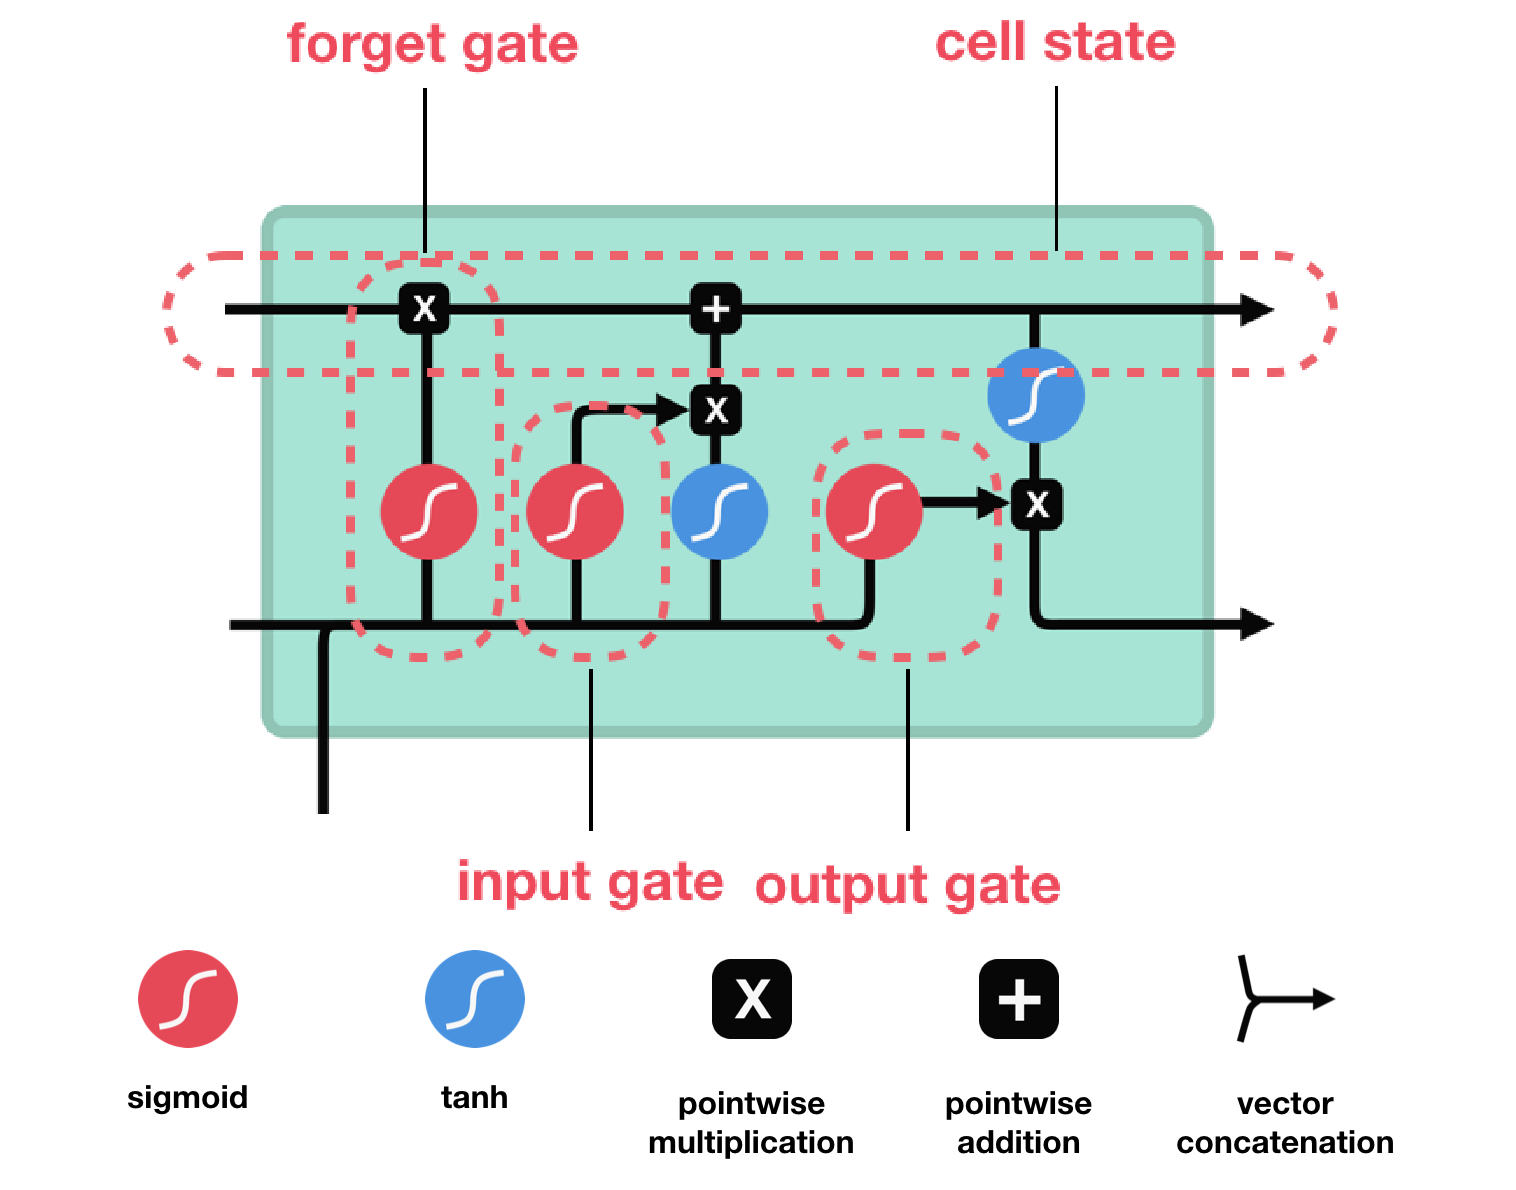
\includegraphics[width=0.8\textwidth]{figuras/fig_9.png}
   \fonte{Adaptado de \cite{Phi2020}}
\end{figure}

\subsection{Gated Recurrent Unit}

A GRU consiste de um tipo de RNN com o mesmo propósito da LSTM, embora considerada uma melhoria em relação a anterior, utilizando menos portas e parâmetros \cite{Kumar2019,Bianchi2017}. Em razão disso, redes GRU superaram a performance de redes LSTM em várias aplicações, treinando e convergindo mais rápido, se mostrando computacionalmente menos custosas e igualmente eficientes \cite{Kumar2019,Bianchi2017}. Empregada também em classificação e previsão de séries temporais, este tipo de rede ajuda na recuperação de informações em escalas de tempo distintas \cite{Bianchi2017,Kumar2019}. 

Cada célula de uma GRU possuí um estado de célula (memória) que utiliza de um estado escondido (\textit{hidden state}) para transferir a informação, com é feito na LSTM. Contudo, a GRU utiliza de apenas duas portas, conforme ilustra a \autoref{fig:cell_gru_gates}: a porta de reinicialização (\textit{reset gate}) e a porta de atualização (\textit{update gate}). A porta de atualização opera de forma similar às portas de esquecimento e a de entrada de uma LSTM, decidindo quais informações descartar e quais informações novas adicionar a memória. A porta de reinicialização, por sua vez, é utilizada para decidir quais informações do passado devem ser esquecidas \cite{Phi2020}.

\begin{figure}[h]
  \centering
  \caption{Componentes de uma célula de GRU.}
   \label{fig:cell_gru_gates}
   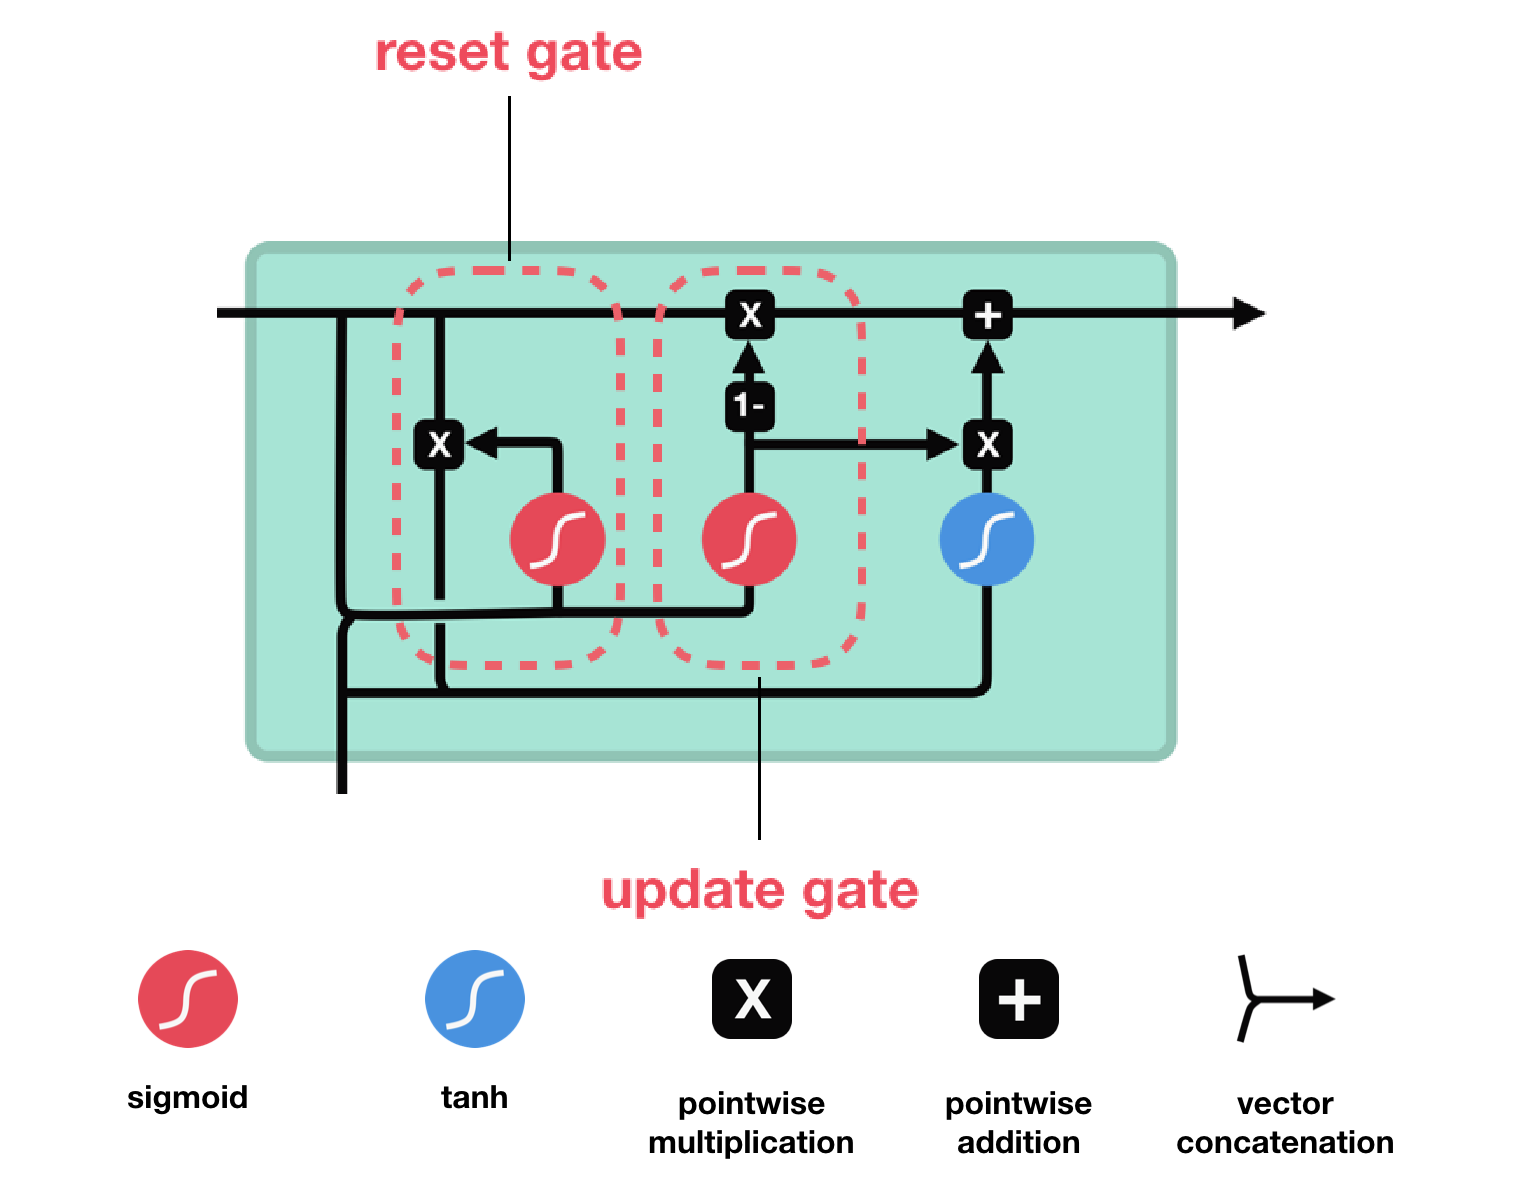
\includegraphics[width=0.8\textwidth]{figuras/fig_10.png}
   \fonte{Adaptado de  \cite{Phi2020}}
\end{figure}

\subsection{Convolutional Neural Network}

A CNN é um tipo de rede neural projetada para tratar eficientemente dados de imagem, se mostrando efetiva em aplicações de visão computacional, como classificação de imagem, localização de objetos, etc. \cite{Brownlee2018}. Através da aplicação de convoluções, este tipo de rede é capaz de aprender como extrair características de alto nível diretamente nos dados brutos, que representam bem os padrões a serem reconhecidos \cite{Dixon2019,Goodfellow2016}. Esta abordagem, denominada \textit{representation learning} \cite{Brownlee2018}, também pode ser aplicada em séries temporais, onde apresenta duas vantagens sobre outras técnicas: dependência local, uma vez que os sinais próximos provavelmente estão correlacionados; e invariância de escala para diferentes passos ou frequências \cite{Wang2019}. Neste tipo de rede, cada camada de convolução possuí uma quantidade \emph{n} de filtros aplicados com um \textit{kernel} de tamanho \emph{m}, conforme ilustra as Figuras \ref{fig:cnn_convolution} e \ref{fig:cnn_convolution_3d}. Após a convolução, geralmente existem camadas de \textit{pooling} e \textit{fully connected}, que executam tarefas de classificação \cite{Wang2019}.

\begin{figure}[h]
  \centering
  \caption{Convolução em dados 1D.}
   \label{fig:cnn_convolution}
   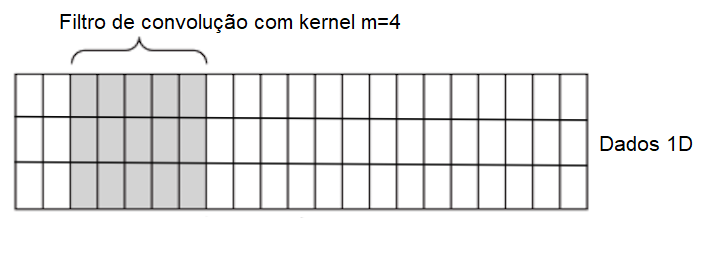
\includegraphics[width=0.9\textwidth]{figuras/fig_11.png}
   \fonte{\cite{Verma2020}}
\end{figure}

\begin{figure}[h]
  \centering
  \caption{Convolução em dados 3D.}
   \label{fig:cnn_convolution_3d}
   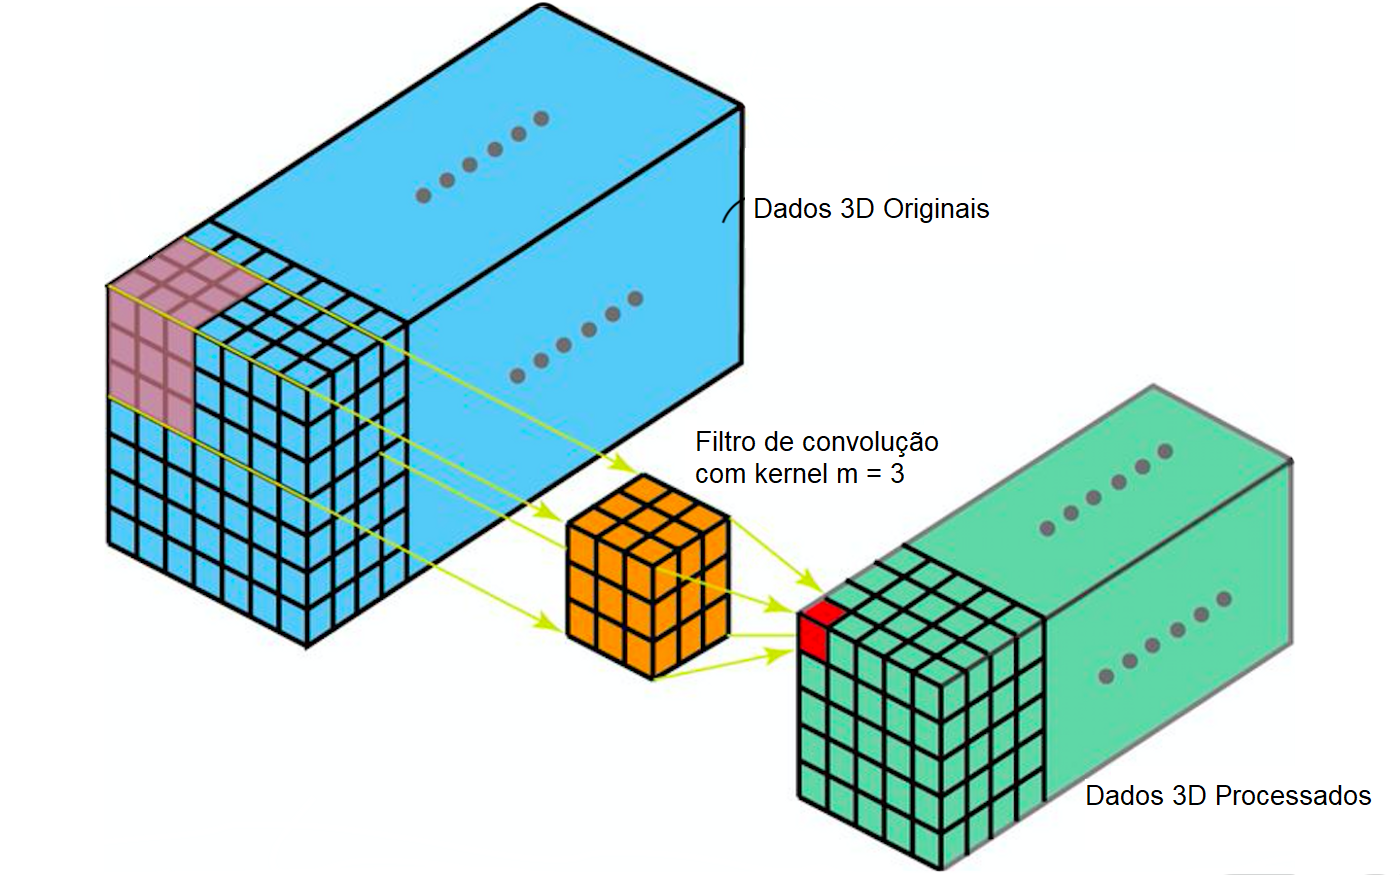
\includegraphics[width=0.8\textwidth]{figuras/fig_12.png}
   \fonte{\cite{Verma2020}}
\end{figure}

\subsection{Convolutional Long Short-Term Memory}

A ConvLSTM é um tipo de RNN variante da LSTM \cite{Salman2018}. Nestas redes existem operações de convolução dentro da célula de LSTM, de forma que as estruturas de convolução são aplicadas tanto na transição de entrada para estado, quanto nas transições de estado para estado. Desta forma, todas as operações de multiplicação de matrizes interna são substituídas por convoluções \cite{Rahman2019}. Neste ponto se mostra evidente a diferença para a híbrida CNN-LSTM, nas quais estruturas de convolução (CNN) são aplicadas como a primeira camada e sequencialmente na segunda camada é aplicada LSTM \cite{Rahman2019}.

\subsection{Convolutional Neural Network Long Short-Term Memory}

A CNN-LSTM constitui um tipo de rede neural híbrida que utiliza de ambas camadas de convolução (CNN) e recorrência (LSTM) \cite{Deep2019}. Nestas redes, os sinais são inicialmente agrupados em sequências temporais, e cada sequência é subdividida em blocos menores, as subsequencias. Nestas subsequências são aplicadas camadas de convolução para extração de características complexas \cite{Deep2019}. Em seguida, estas características são agrupadas novamente na sequência original e empregadas em camadas recorrentes, para interpretar a sequência temporal das características produzidas.

\section{Métricas de Avaliação}

Para mensurar os resultados dos experimentos foram adotadas métricas comumente utilizadas em problemas de classificação: acurácia, precisão, \textit{recall} e \textit{f1-score} \cite{Rodrigues2020,Rodrigues2021,Shung2020}. Em um problema de classificação, os resultados podem ser classificados em Verdadeiros Positivos (VP), sendo a classificação correta da classe Positivo; Verdadeiros Negativos (VN), a classificação correta da classe Negativo; Falsos Positivos (FP), erro em que o modelo previu a classe Positivo quando o valor real era classe Negativo; e Falsos Negativos (FN), erro em que o modelo previu a classe Negativo quando o valor real era classe Positivo \cite{Rodrigues2020}. A \autoref{fig:classificacao_positivo_negativo} ilustra os resultados possíveis.

\begin{figure}[h]
  \centering
  \caption{Matriz confusão de classificação.}
   \label{fig:classificacao_positivo_negativo}
   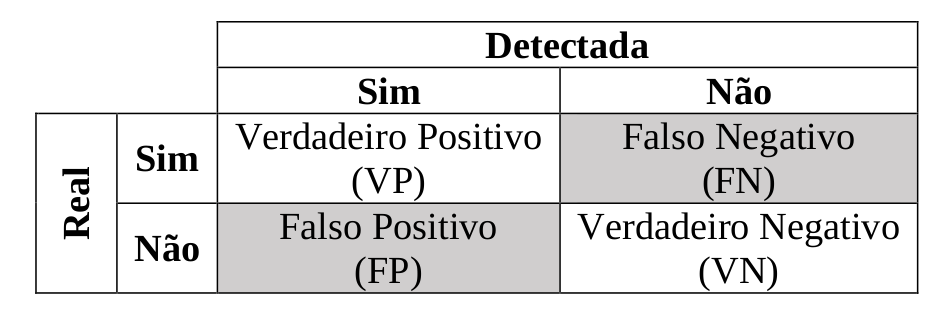
\includegraphics[width=0.6\textwidth]{figuras/fig_13.png}
   \fonte{\cite{Rodrigues2020}}
\end{figure}

A acurácia indica uma performance geral do modelo. Desta forma, consiste da proporção de amostras classificadas corretamente em relação ao total de amostras, considerando todas as classes de dados. A fórmula desta métrica é apresentada a seguir:

\begin{center}
  \[
  \textit{Acurácia} = \frac{VP + VN}{VP + VN + FP + FN}
  \]
\end{center}

Por outro lado, as métricas de precisão, \textit{recall} e \textit{f1-score} avaliam cada uma das classes de dados separadamente, de modo que se possa verificar problemas de desbalanceamento e viés. A precisão mede a proporção de amostras preditas corretamente em relação ao total de predições para determinada classe de dados, conforme a seguinte fórmula:

\begin{center}
  \[
  \textit{Precisão} = \frac{VP}{VP + FP}
  \]
\end{center}

A \textit{recall} mede a proporção de amostras preditas corretamente para determinada classe de dados em relação a todas as amostras reais daquela classe, conforme a seguinte fórmula:

\begin{center}
  \[
  \textit{Recall} = \frac{VP}{VP + FN}
  \]
\end{center}

Por fim, a \textit{f1-score} consiste da média harmônica de precisão e \textit{recall}, conforme a fórmula a seguir:

\begin{center}
  \[
  \textit{F1-Score} = \frac{2 * \textit{precisão} * \textit{recall}}{\textit{precisão} + \textit{recall}}
  \]
\end{center}

\chapter{Proposta}
\label{cap:proposta}

Nesta seção é detalhada a proposta de modelo adaptativo a ser desenvolvido de percepção veicular de ambiente e propriocepção veicular. Nas próximas seções é detalhada a metodologia e materiais adotados, andamento da pesquisa, resultados preliminares obtidos e cronograma de atividades.

\section{Metodologia}

Para o desenvolvimento deste trabalho, inicialmente foi realizado o levantamento do estado-da-arte sobre percepção veicular de ambiente e propriocepção veicular, através de sinais de sensores inerciais. Este levantamento se deu por intermédio de produção de uma Revisão Sistemática da Literatura (RSL), em bases de dados relevantes na área de computação. Através dessa sistemática, diversas lacunas de pesquisa foram identificadas conforme discorrido no capítulo \ref{cap:revisao}, com a delimitação de escopo desta pesquisa. Baseando-se nas lacunas de pesquisa, o desenvolvimento da metodologia de percepção adaptativa se dá em três etapas, sendo elas a coleta de dados, o pré-processamento e processamento. 

Na etapa de de coleta de dados, são utilizadas duas redes de sensores no veículo, sendo cada uma destas constituídas por um \textit{Single-Board Computer} (SBC) Raspberry Pi e três placas MPU-9250, cada uma equipada com um acelerômetro, um giroscópio e um magnetômetro. Também foi utilizado uma fonte externa de GPS, com produção de dados de localização e velocidade. Para definição dos referenciais, utilizou-se posicionamento controlado, uma vez que melhor se adéqua ao estudo. Sendo assim, o posicionamento das placas foi realizado de forma que os eixos do referencial do sensor coincidem com os do veículo, não sendo necessário mapear. As redes com as placas MPU-9250 foram distribuídas no veículo de forma a considerar os dados provindos de pontos com diferentes fatores de dependência, uma vez que a análise busca estabelecer qual ponto fornece os dados que produzem melhores resultados. Sendo assim, foram distribuídas no veículo da seguinte maneira: cada extremidade do eixo frontal (lado direito e esquerdo) recebeu uma das redes, onde anexou-se uma placa na bandeja da suspensão, localizando-se abaixo e próximo à suspensão veicular; outra placa acima e próxima à suspensão, anexada na lataria; e outra placa anexada na \textit{dashboard} do veículo, dentro da cabine. A taxa de amostragem não foi restringida, atingindo próximo a 1 kHz, uma vez que para os experimentos será realizado \textit{downsampling} para verificar a melhor taxa. Foi empregada a faixa de medição máxima (8g), uma vez que em testes exploratórios foi observado em algumas ocasiões a produção de valores de até aproximadamente 7.5g. 

Após, na etapa de pré-processamento se busca melhorar os dados brutos antes de serem parametrizados a técnica de reconhecimento de padrões. Sendo assim, será utilizada técnica empregada por \cite{Li2018} para aproximar as localizações e velocidade em uma taxa próxima a dos sensores inerciais. Desta forma, são produzidos dados mais próximos aos reais em cada amostra. Nesta etapa também será integrado o modelo matemático \textit{Quarter Car}, de forma que suas fórmulas condicionem os valores dos sensores inerciais ao veículo no qual os dados foram captados. Também será investigado se o emprego de formalismos matemáticos que descrevem as relações físicas entre as variáveis, como aceleração centrífuga a partir da aceleração, velocidade e curvatura, podem melhorar os resultados se aplicados como pré-processamento, ao invés de deixar a rede neural descobrir suas relações.

Na etapa de processamento serão aplicadas os dados pré-processados à uma técnica de \textit{Deep Learning}, sendo ela redes neurais recorrentes do tipo LSTM. Com o desenvolvimento das percepções, serão fornecidas as mesmas como mais uma das entradas para outras percepções, como forma de verificar melhorias dado sua correlação. A validação da adaptabilidade será feita com base nos \textit{datasets} produzidos na primeira etapa. Para isso, serão coletados ao menos quatro conjuntos de dados com diferenças de propriedades veiculares, de ambiente e de condução. Três dos \textit{datasets} serão utilizados parcialmente para treinamento e o restante para validação, sendo o quarto \textit{dataset} utilizados somente para validação, de forma a verificar o comportamento do modelo em um contexto desconhecido.

\section{Andamento da Proposta e Resultados Preliminares}

A pesquisa prática encontra-se em estágio inicial de desenvolvimento. Foi produzido para os testes preliminares um \textit{dataset} com os quais foram aplicados reconhecimento de algumas percepções. Este \textit{dataset} é composto de dados amostrados no seguinte contexto: um veículo trafegando em vias com três diferentes tipos de superfície, com a presença de eventos transientes como buracos, lombadas, curvas, etc., com variações no modo de condução, tal como diferentes velocidades. Utilizando-se deste \textit{dataset}, foram produzidas três percepções veiculares diferentes, a fim de demonstrar ser possível realizar este tipo de reconhecimento nos dados dos sensores, assim como validar que a técnica de \textit{Deep Learning} proposta é adequada ao problema de pesquisa. Os reconhecimentos realizados foram dois de percepção de ambiente, sendo um evento persistente de tipo de composição de superfície e outro transiente, sendo as lombadas; e um reconhecimento de propriocepção, o evento transiente de curvas.

Para realização dos testes, após a criação de diversos modelos de redes neurais profundas, chegou-se a rede detalhada na Figura \ref{fig:rede_proposta}. Esta rede é composta de uma camada de entrada, a qual recebe sequencias de 25 amostras (2,5 segundos) para formação da saída. São parametrizadas sete variáveis, sendo aceleração e rotação nos três eixos captados abaixo da suspensão veicular, e a velocidade. Posteriormente, estes dados passam para uma camada de convolução, a fim de filtrá-los e melhorá-los. Nesta etapa, estudos anteriores geralmente empregaram métodos estatísticos, tais como média móvel simples, para suavizar os dados e remover ruídos. Em seguida, os dados são parametrizados a duas camadas de LSTM, conhecidas como \textit{stacked} LSTM. Estas camadas são responsáveis por extrair as características dos dados. Alguns estudos anteriores empregaram nesta etapa métodos como o desvio padrão, para extração de característica de vibração dos sinais. Por fim, os dados são passados a camada de saída, resultando em uma ou mais classes, conforme a percepção produzida.

\begin{figure}[h!]
  \centering
  \caption{Rede Neural Profunda.}
   \label{fig:rede_proposta}
   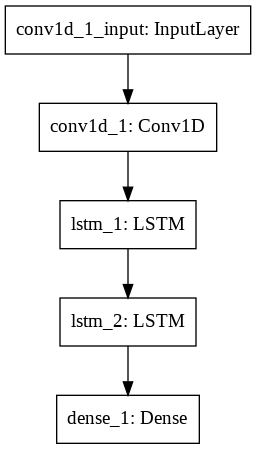
\includegraphics[width=0.3\textwidth]{figuras/fig4_2.png}
   \fonte{O autor.}
\end{figure}

O primeiro teste se concentrou no reconhecimento do tipo de superfície da vida. Foram reconhecidos três tipos diferentes, sendo pavimento rígido (asfalto), pavimento flexível (paralelepípedo ou hexagonal) e sem pavimentação (terra). A rede neural profunda para este reconhecimento obteve uma acurácia de 99\%, com um Erro Médio Quadrático (\textit{Mean Squared Error} - MSE) de 0.0000045885. O reconhecimento de pavimento asfáltico obteve o melhor resultado, com Erro Médio Absoluto (\textit{Mean Absolute Error} - MAE) de 0.000023. Em seguida, o reconhecimento de terra obteve MAE de 0.000054, e o reconhecimento de paralelepípedo/hexagonal obteve MAE de 0.000064. As Figuras \ref{fig:resultado_asfalto}, \ref{fig:resultado_paralelepipedo} e \ref{fig:resultado_terra} detalham os resultados.

O segundo teste foi voltado ao reconhecimento de lombadas. Sendo assim, envolveu lombadas tanto em pavimento asfáltico, quando em paralelepípedo, de diversas dimensões. A rede neural profunda para esse reconhecimento também obteve acurácia de 99\% e um MSE de 0.0005878024. O MAE foi de 0.000012, e os resultados são detalhados na Figura \ref{fig:resutlado_lombada}. Por fim, no terceiro teste foi realizado o reconhecimento de curvas à direita e à esquerda, sendo elas leves ou acentuadas. A rede obteve acurácia de 92\% com um MSE de 0.0020476580. Para curvas a esquerda, o MAE foi de 0.004028, e para a direita, de 0.010060. Os resultados são detalhados na Figura \ref{fig:resultado_curva_esquerda} e \ref{fig:resultado_curva_direita}.

De modo geral, é possível observar o bom desempenho a rede em filtrar sinais, extrair características e reconhecer os padrões, fazendo com que a LSTM seja interessante para este problema. Em relação à adaptabilidade, alguns fatores de dependência já foram agregados, como a velocidade e características sensoriais descritas na seção anterior. Sendo assim, faltam agregar os demais fatores ao modelo, e prosseguir com testes para outras percepções e outros contextos, com a produção de novos \textit{datasets}.

\begin{figure}[h!]
  \centering
  \caption{Reconhecimento de Pavimento Rígido (Asfalto).}
   \label{fig:resultado_asfalto}
   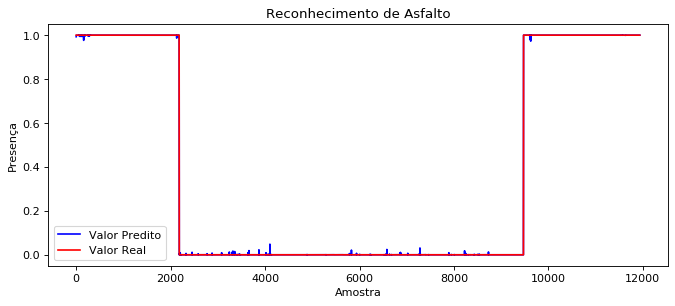
\includegraphics[width=1\textwidth]{figuras/fig4_2_1.png}
   \fonte{O autor.}
\end{figure}

\begin{figure}[h!]
  \centering
  \caption{Reconhecimento de Pavimento Flexível (Hexagonal ou Paralelepípedo).}
   \label{fig:resultado_paralelepipedo}
   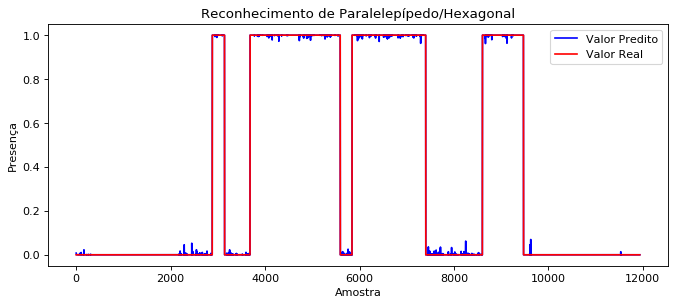
\includegraphics[width=1\textwidth]{figuras/fig4_2_2.png}
   \fonte{O autor.}
\end{figure}

\begin{figure}[h!]
  \centering
  \caption{Reconhecimento de Sem Pavimento (Terra).}
   \label{fig:resultado_terra}
   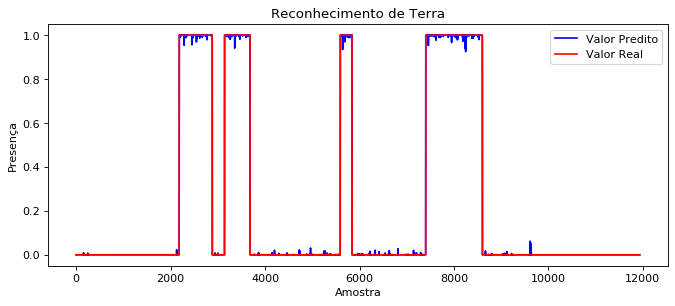
\includegraphics[width=1\textwidth]{figuras/fig4_2_3.png}
   \fonte{O autor.}
\end{figure}

\begin{figure}[h!]
  \centering
  \caption{Reconhecimento de Lombada.}
   \label{fig:resutlado_lombada}
   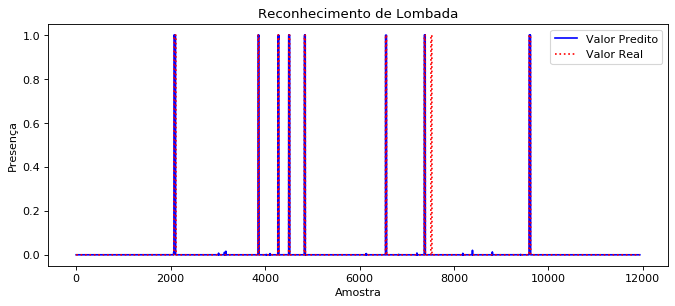
\includegraphics[width=1\textwidth]{figuras/fig4_2_4.png}
   \fonte{O autor.}
\end{figure}

\begin{figure}[h!]
  \centering
  \caption{Reconhecimento de Curva à Esquerda.}
   \label{fig:resultado_curva_esquerda}
   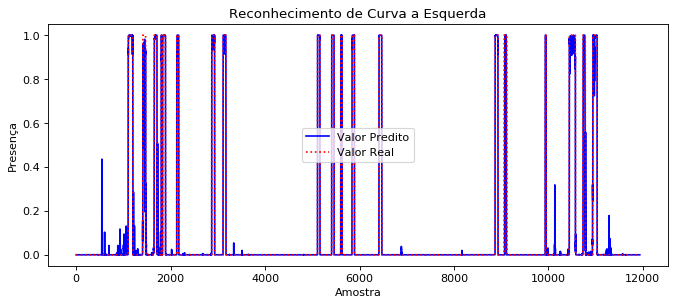
\includegraphics[width=1\textwidth]{figuras/fig4_2_5.png}
   \fonte{O autor.}
\end{figure}

\begin{figure}[h!]
  \centering
  \caption{Reconhecimento de Curva à Direita.}
   \label{fig:resultado_curva_direita}
   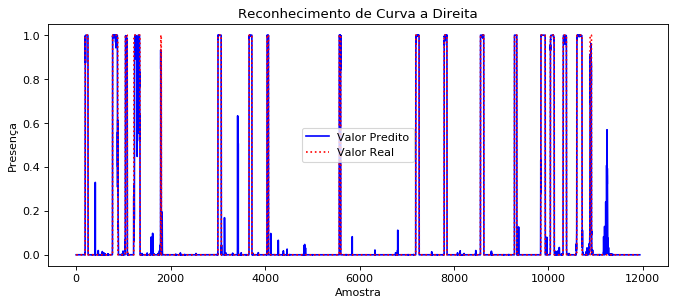
\includegraphics[width=1\textwidth]{figuras/fig4_2_6.png}
   \fonte{O autor.}
\end{figure}

\clearpage 
\section{Cronograma}

Abaixo é apresentado o cronograma a ser seguido com o intuito de cumprir as etapas da pesquisa e os requisitos que regulamentam o curso.

\begin{figure}[h!]
  \centering
  \caption{Cronograma de atividades.}
   \label{fig:proprioception_occurrence}
   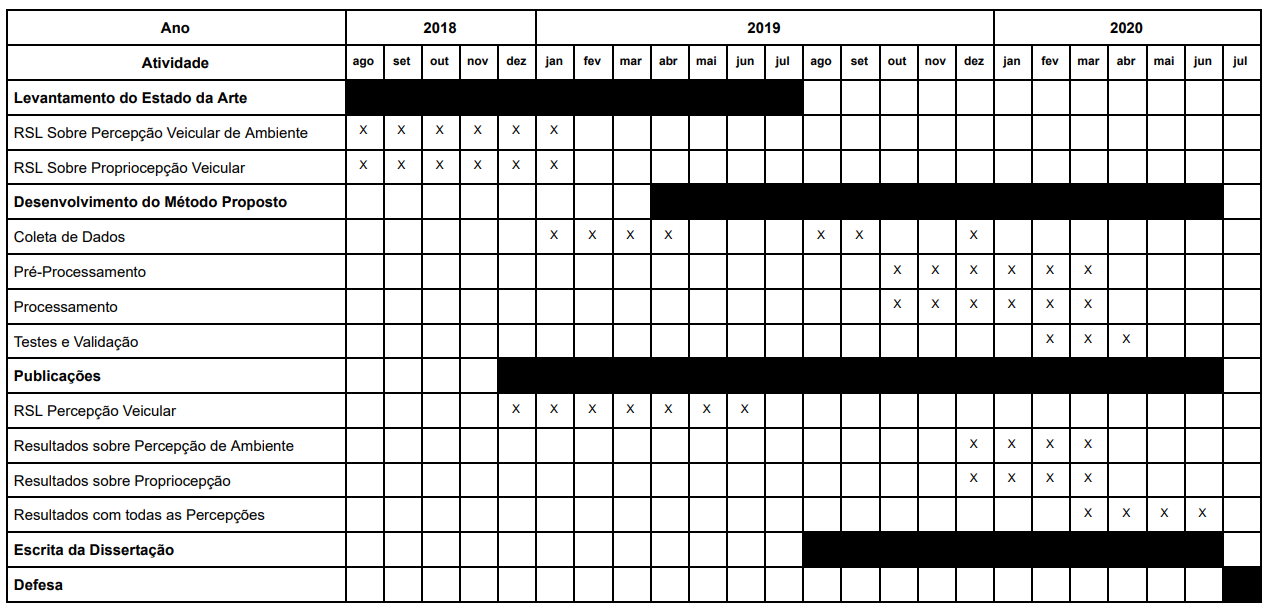
\includegraphics[width=1\textwidth]{figuras/fig4.png}
   \fonte{O autor.}
\end{figure}


\chapter{Conjuntos de Dados}
\label{cap:conjuntos_de_dados}

Para realizar os experimentos deste estudo foi necessário dispor de conjuntos de dados amostrados através de sensores de abordagem passiva, aplicados em variações contextuais relacionadas aos fatores de dependência. Sendo assim, inicialmente realizamos o levantamento das principais bases de dados utilizadas em estudos envolvendo aplicações de ITS. Baseando-se em revisões anteriores \cite{Geyer2020}, elencamos características necessárias para condução dos experimentos e avaliamos a aderência à elas dos conjuntos de dados disponíveis. Embora os conjuntos possuam outros sensores, nossa análise focou-se nos de abordagem passiva.

Na \autoref{tabela:datasets} é detalhado a comparação. São utilizados os marcadores \emph{Sim (S)}, \emph{Não (N)} e \emph{Indefinido (I)}. São considerados \emph{S} os conjuntos que cumprem todos os requisitos de determinada característica, \emph{N} aqueles que não cumprem ao menos uma restrição, e \emph{I} quando não foi possível identificar informações do parâmetro avaliado. Na avaliação dos sensores inerciais e magnetômetro, foi considerado como requisito os conjuntos possuírem dados brutos nos três eixos. Para diferentes veículos, o requisito foi de utilizar diferentes modelos. Para ambientes, considerou-se diferentes superfícies, com variação de pavimentações ou não pavimentação. Para colocações, o requisito embelecido torna necessário ao menos um conjunto de sensores inerciais abaixo da suspensão e um acima. Por fim, o posicionamento controlado é requerido por produzir dados de forma mais confiável e permitir análises de propriocepção e exterocepção.

\begin{table}[h!]
    \small
    \centering
    \caption{Comparação de conjuntos de dados públicos}
    \label{tabela:datasets}
    \begin{tabular}{llcccccc}
\cmidrule(l){3-8}
 &  & \multicolumn{6}{c}{\textbf{Conjunto de Dados}} \\ \cmidrule(l){3-8} 
 & \textbf{} 
 & \textit{\href{http://www.cvlibs.net/datasets/kitti/setup.php}{KITTI}} 
 & \textit{\href{http://apolloscape.auto/index.html}{Apollo Scape}} 
 & \textit{\href{https://www.nuscenes.org/}{nuScenes}} 
 & \textit{\href{https://self-driving.lyft.com/level5/data/}{Lyft Level 5}} 
 & \textit{\href{https://waymo.com/open/}{Waymo}} 
 & \textit{\href{https://www.a2d2.audi/a2d2/en.html}{A2D2}} \\ \midrule
\multirow{5}{*}{\rotatebox[origin=c]{90}{\textbf{Sensores}}} & \textit{Câmera} & S & S & S & S & S & S \\ \cmidrule(l){2-8} 
 & \textit{GPS} & S & S & S & N & N & S \\ \cmidrule(l){2-8} 
 & \textit{Acelerômetro 3D} & S & S & N & N & N & S \\ \cmidrule(l){2-8} 
 & \textit{Giroscópio 3D} & S & S & S & N & N & N \\ \cmidrule(l){2-8} 
 & \textit{Magnetômetro 3D} & N & N & N & N & N & N \\ \midrule
\multirow{5}{*}{\rotatebox[origin=c]{90}{\textbf{Contexto}}} & \textit{Diferentes Veículos} & N & I & N & I & I & I \\ \cmidrule(l){2-8} 
 & \textit{Diferentes Condutores} & I & I & I & I & I & I \\ \cmidrule(l){2-8} 
 & \textit{Diferentes Ambientes} & I & I & I & I & I & I \\ \cmidrule(l){2-8} 
 & \textit{Diferentes Colocações} & N & N & N & N & N & N \\ \cmidrule(l){2-8} 
 & \textit{Posicionamento Controlado} & S & I & S & N & N & I \\ \bottomrule
\end{tabular}
    \fonte{Desenvolvido pelo autor.}
\end{table}

Conforme observado na análise comparativa, nenhum dos conjuntos de dados disponíveis apresentam dados para todos os sensores necessários, dentre sensores inerciais e de suporte. Na análise de contexto as características avaliadas se mostram ainda menos presentes, especialmente por conta de os sensores inerciais não serem o foco de nenhum dos conjuntos e, portanto, sua abordagem de coleta não ser tratada de forma adequada. Em geral, as propriedades avaliadas como \emph{I} são propensas a serem \emph{N}, uma vez que sua não especificação tende a ter sido em razão de não ser considerada ou não existir. Em uma análise ampla, nenhum dos conjuntos de dados avaliados atende os requisitos para experimentação deste estudo e, por isso, se fez necessário conduzir uma etapa de coleta de dados, detalhada nas próximas subseções.

\section{Rede de Sensores}

Para coletar os dados foram desenvolvidas duas redes de sensores, sendo cada uma delas composta por um SBC Raspberry Pi e três módulos MPU-9250, cada um deles equipado com um acelerômetro 3D, giroscópio 3D, magnetômetro 3D e um sensor de temperatura. Uma fonte externa de GPS também foi utilizada, produzindo dados de localização e velocidade, assim como uma câmera para captura de vídeo do ambiente. A \autoref{tabela:rede_de_sensores} detalha o \textit{hardware} utilizado.

\begin{table}[h!]
\small
\caption{Hardware da rede de sensores} 
\label{tabela:rede_de_sensores}
\centering
\begin{tabular}{llll}
\toprule
\multicolumn{1}{l}{\textbf{Hardware}} & 
\multicolumn{1}{l}{\textbf{Sensor}} & 
\multicolumn{1}{l}{\textbf{Dados}} & 
\multicolumn{1}{l}{\textbf{Taxa}}  
\\ \midrule

\multicolumn{1}{l}{HP Webcam HD-4110} & 
\multicolumn{1}{l}{Câmera} & 
\multicolumn{1}{l}{Vídeo 720p} & 
\multicolumn{1}{c}{30 Hz}                   
\\ \midrule

\multicolumn{1}{l}{Xiaomi Mi 8} & 
\multicolumn{1}{l}{GPS} & 
\multicolumn{1}{l}{Velocidade em $m/s$, latitude, longitude, etc.} &
\multicolumn{1}{c}{1 Hz}
\\ \midrule

\multicolumn{1}{l}{\multirow{5}{*}{MPU-9250}} & 
\multicolumn{1}{l}{Acelerômetro} & 
\multicolumn{1}{l}{Aceleração 3D em $m/s^2$} &
\multicolumn{1}{c}{\multirow{5}{*}{100 Hz}} 
\\ \cmidrule(lr){2-3}

\multicolumn{1}{l}{} & 
\multicolumn{1}{l}{Giroscópio} & 
\multicolumn{1}{l}{Taxa de rotação 3D em $graus/s$} & 
\multicolumn{1}{l}{}                       
\\ \cmidrule(lr){2-3}

\multicolumn{1}{l}{} & 
\multicolumn{1}{l}{Magnetômetro} & 
\multicolumn{1}{l}{Campo geomagnético ambiente 3D em $\mu T$} & 
\multicolumn{1}{l}{}
\\ \cmidrule(lr){2-3}

\multicolumn{1}{l}{} & 
\multicolumn{1}{l}{Temperatura} &
\multicolumn{1}{l}{Temperatura em $^{\circ}C$} & 
\multicolumn{1}{l}{}                       
\\ \bottomrule

\end{tabular}
\fonte{Desenvolvido pelo autor.}
\end{table}

Todo o equipamento foi fixado no veículo conforme detalha a \autoref{fig:colocacao_posicionamento_rede_sensores}. A câmera foi colocada na parte externa do teto do carro (1), capturando vídeo do ambiente em 30Hz. O receptor GPS foi colocado internamente no painel (2), amostrando dados em 1Hz. Os seis módulos MPU-9250 foram distribuídos no veículo de forma a considerar os dados provindos de pontos com diferentes influências da propriedade de dependência veicular. Sendo assim, em ambas as extremidades do eixo dianteiro (lado direito e esquerdo) foi anexado um módulo ao braço de controle (4), localizado abaixo e próximo à suspensão do veículo; outro módulo foi colocado acima e próximo da suspensão, anexado à carroceria imediatamente acima do pneu (3); e outro módulo foi anexado no painel do veículo (2), dentro da cabine. Em relação ao referencial de amostragem dos módulos MPU-9250, foi utilizada a abordagem de posicionamento controlado, onde a colocação dos módulos foi realizada de forma que os três eixos do sistema de coordenadas do sensor ficaram alinhados com os do veículo, sendo tanto referencial de coleta como de análise. O acelerômetro foi ajustado em um \textit{Full Scale Range} (FSR) de 8$g$ e o giroscópio de 1000$graus/s$, constituindo intervalos consistentes para não saturar, ambos amostrando em 100Hz (propriedades sensoriais).

\begin{figure}[h!]
  \centering
  \caption{Colocação e posicionamento da rede de sensores no veículo}
   \label{fig:colocacao_posicionamento_rede_sensores}
   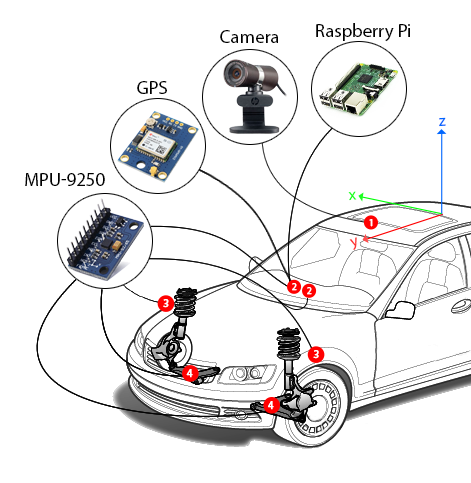
\includegraphics[width=0.69\textwidth]{figuras/fig_22.png}
   \fonte{Desenvolvido pelo autor.}
\end{figure}

\section{Execução da Coleta}

Para o desenvolvimento e validação de modelos de percepção veicular adaptativa, se mostrou necessário produzir dados em variações contextuais para obter variabilidade de condições relacionadas aos fatores de dependência. Sendo assim, além da amostragem de velocidade (propriedade de condução) e da colocação dos sensores inerciais em diferentes pontos da estrutura veicular (propriedade veicular), nós realizamos diversas coletas de dados utilizando da rede de sensores em três diferentes modelos de veículos (propriedade veicular), com três diferentes motoristas variando a velocidade de 0 \emph{km/h} até 91.98 \emph{km/h} (propriedade de condução) trafegando em três cenários distintos (propriedade ambiental). Cada cenário contém vias sem pavimentação (terra) e trechos pavimentados (asfalto ou paralelepípedo), com variações gerais do ambiente, tais como presença de lombadas, buracos, diferentes níveis de conservação do pavimento, etc. Detalhes dos cenários são apresentados na próxima seção. Sendo assim, foram produzidos nove conjuntos de dados denominados \textit{Passive Vehicular Sensors Dataset} (PVS 1-9), detalhados na \autoref{table:descricao_conjuntos}. Cada um dos conjuntos de dados é composto pelos arquivos especificados na \autoref{table:conjuntos_arquivos}. Os dados foram coletados no município de Anita Garibaldi, no interior do estado de Santa Catarina, Brasil, entre os dias 24 e 26 de dezembro de 2019. O ponto médio dos cenários é dado pelas coordenadas (-27.69983094872972, -51.11577673365139).

\begin{table}[H]
\small
\caption{Conjuntos de dados produzidos} 
\label{table:descricao_conjuntos}
\centering
\begin{tabular}{llll}
\toprule
\textbf{Nome} & \textbf{Veículo} & \textbf{Condutor} & \textbf{Cenário} \\ \midrule
PVS 1 & Volkswagen Saveiro & Condutor 1 & Cenário 1 \\ \midrule
PVS 2 & Volkswagen Saveiro & Condutor 1 & Cenário 2 \\ \midrule
PVS 3 & Volkswagen Saveiro & Condutor 1 & Cenário 3 \\ \midrule
PVS 4 & Fiat Bravo & Condutor 2 & Cenário 1 \\ \midrule
PVS 5 & Fiat Bravo & Condutor 2 & Cenário 2 \\ \midrule
PVS 6 & Fiat Bravo & Condutor 2 & Cenário 3 \\ \midrule
PVS 7 & Fiat Palio & Condutor 3 & Cenário 1 \\ \midrule
PVS 8 & Fiat Palio & Condutor 3 & Cenário 2 \\ \midrule
PVS 9 & Fiat Palio & Condutor 3 & Cenário 3 \\ \bottomrule
\end{tabular}
\fonte{Desenvolvido pelo autor.}
\end{table}

\vspace{-1.1cm}

\begin{table}[H]
\small
\caption{Arquivos que compõe cada conjunto de dados} 
\label{table:conjuntos_arquivos}
\centering
\begin{tabular}{ll}
\toprule
\textbf{Arquivo} & \textbf{Descrição} \\ \midrule
dataset\_gps.csv & Dados de GPS, incluindo latitude, longitude, altitude, velocidade, \\ & acurácia, etc. \\ \midrule
dataset\_gps\_mpu\_left.csv & Dados dos MPUs colocados no lado esquerdo do veículo, \\ & combinados com dados GPS. \\ \midrule
dataset\_gps\_mpu\_right.csv & Dados dos MPUs colocados no lado direito do veículo, \\ & combinados com dados GPS. \\ \midrule
dataset\_labels.csv & Classes de dados para cada amostra do conjunto de dados \\ & (para ambos os lados). \\ \midrule
dataset\_mpu\_left.csv & Dados dos MPUs colocados no lado esquerdo do veículo. \\ \midrule
dataset\_mpu\_right.csv & Dados dos MPUs colocados no lado direito do veículo. \\ \midrule
dataset\_settings\_left.csv & Configurações dos MPUs colocados no lado esquerdo \\ & do veículo. Inclui faixa de medição, resolução, etc. \\ \midrule
dataset\_settings\_right.csv & Configurações dos MPUs colocados no lado direito \\ & do veículo. Inclui faixa de medição, resolução, etc. \\ \midrule
map.html & Mapas interativos com os dados e as classes. \\ \midrule
video\_dataset\_left.mp4 & Vídeo com gráficos dos dados dos MPUs e GPS, amostrados \\ & no lado esquerdo do veículo. \\ \midrule
video\_dataset\_right.mp4 & Vídeo com gráficos dos dados dos MPUs e GPS, amostrados \\ & no lado direito do veículo. \\ \midrule
video\_environment.mp4 & Vídeo do ambiente externo. \\ \midrule
video\_environment\_dataset\_left.mp4 & Vídeos lado a lado de video\_environment.mp4 e \\ & video\_dataset\_left.mp4 \\ \midrule
video\_environment\_dataset\_right.mp4 & Vídeos lado a lado de video\_environment.mp4 e \\ & video\_dataset\_right.mp4 \\ \bottomrule
\end{tabular}
\fonte{Desenvolvido pelo autor.}
\end{table}

\section{Classes de Dados}

Para criação dos rótulos correspondentes às classes de dados, foram utilizados GT de anotação humana e de anotação automatizada por máquina. Os primeiros rótulos criados foram os das classes de dados de tipo de superfície de pista. Para essas classes, foram criados os rótulos \emph{terra} (dirt\_road), \emph{paralelepípedo} (cobblestone\_road) e \emph{asfalto} (asphalt\_road). A anotação foi realizada via GT humano, uma vez que esta classe representa uma característica objetiva. Desta forma, através da observação do que a roda toca por meio do vídeo capturado, os delimitadores de início e fim dessas classes puderam ser facilmente apontados. A \autoref{fig:tipos_superficie} ilustra os tipos de superfície presentes em todos os conjuntos de dados PVS, com a \autoref{fig:mapa_superficies} detalhando a distribuição delas no mapa de cada cenário. A \autoref{table:tipos_superficie_metricas} detalha as métricas para cada conjunto, com a quantificação das amostras e a proporção da distribuição das classes de dados, informações importantes para se analisar o nível de desbalanceamento das classes antes do treinamento dos modelos. 

\begin{figure}[H]
  \centering
  \caption{Tipos de superfície presentes nos cenários}
   \label{fig:tipos_superficie}
   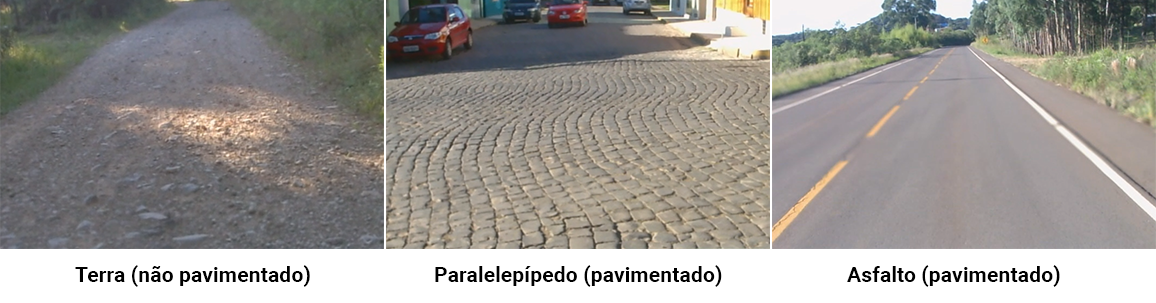
\includegraphics[width=1\textwidth]{figuras/fig_23.png}
   \fonte{Desenvolvido pelo autor.}
\end{figure}

\begin{figure}[H]
  \centering
  \caption{Mapa das superfícies presentes nos cenários.}
   \label{fig:mapa_superficies}
   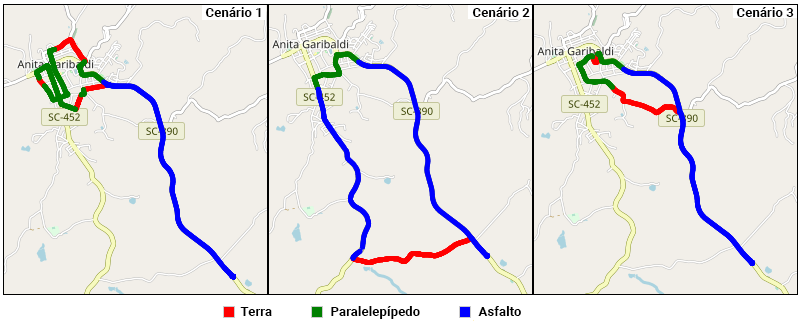
\includegraphics[width=1\textwidth]{figuras/fig_25.png}
   \fonte{Desenvolvido pelo autor.}
\end{figure}

\begin{table}[H]
\scriptsize
\centering
\caption{Métricas para as classes de dados de tipo de superfície} 
\label{table:tipos_superficie_metricas}
\begin{tabular}{ccccccccc}
\cmidrule(l){3-9} & & 
\multicolumn{4}{c}{\textbf{Número de Amostras}} & 
\multicolumn{3}{c}{\textbf{Distribuição das Classes de Dados (\%)}} 
\\ \midrule

\multicolumn{1}{c}{\textbf{Cenário}} &
\textbf{Conjunto} &
\textbf{Terra} &
\textbf{Paralelepípedo} &
\textbf{Asfalto} & 
\textbf{Total} &
\textbf{Terra} &
\textbf{Paralelepípedo} &
\textbf{Asfalto}
\\ \midrule

\multicolumn{1}{c}{\multirow{4}{*}{1}} & PVS 1 & 25868 & 61659 & 56509 & 144036 & 17.96 & 42.81 & 39.23 \\ \cmidrule(l){2-9} 
\multicolumn{1}{c}{} & PVS 4 & 23903 & 57670 & 50919 & 132492 & 18.04 & 43.53 & 38.43 \\ \cmidrule(l){2-9} 
\multicolumn{1}{c}{} & PVS 7 & 23778 & 54224 & 50546 & 128548 & 18.50 & 42.18 & 39.32 \\ \midrule

\multicolumn{1}{c}{\multirow{4}{*}{2}} & PVS 2 & 44618 & 20737 & 59330 & 124685 & 35.78 & 16.63 & 47.58 \\ \cmidrule(l){2-9} 
\multicolumn{1}{c}{} & PVS 5 & 60539 & 18143 & 55195 & 133877 & 45.22 & 13.55 & 41.23 \\ \cmidrule(l){2-9} 
\multicolumn{1}{c}{} & PVS 8 & 44939 & 18825 & 59854 & 123618 & 36.35 & 15.23 & 48.42 \\ \midrule

\multicolumn{1}{c}{\multirow{4}{*}{3}} & PVS 3 & 28659 & 26143 & 51014 & 105816 & 27.08 & 24.71 & 48.21 \\ \cmidrule(l){2-9} 
\multicolumn{1}{c}{} & PVS 6 & 23888 & 31641 & 40750 & 96279 & 24.81 & 32.86 & 42.32 \\ \cmidrule(l){2-9} 
\multicolumn{1}{c}{} & PVS 9 & 23153 & 25182 & 43220 & 91555 & 25.29 & 27.50 & 47.21 \\ \bottomrule

\end{tabular}
\fonte{Desenvolvido pelo autor.}
\end{table}

O segundo grupo de classes de dados rotuladas foi o de lombadas. Assim como as classes de tipo de superfície, as de lombadas correspondem a características objetivas e foram anotadas com GT humano. Foram criados os rótulos \emph{com lombada} (asphalt\_speed\_bump e cobblestonne\_speed\_bump), e \emph{sem lombada} (no\_speed\_bump). As lombadas foram amostradas nos dois tipos de pavimentação, conforme ilustra a \autoref{fig:lombadas_superficies}. A \autoref{fig:lombadas_mapa} detalha as localizações das lombadas, e a \autoref{table:lombada_metricas} especifica as métricas destas classes de dados.

\begin{figure}[h!]
  \centering
  \caption{Lombadas em diferentes superfícies presentes nos cenários}
   \label{fig:lombadas_superficies}
   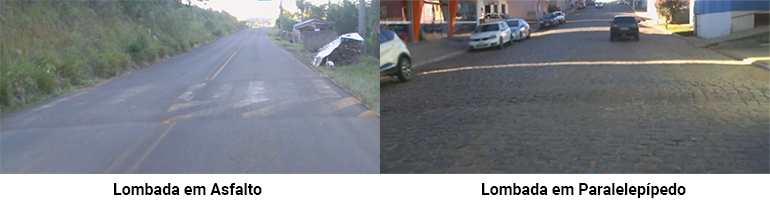
\includegraphics[width=0.85\textwidth]{figuras/fig_24.png}
   \fonte{Desenvolvido pelo autor.}
\end{figure}

\begin{figure}[h!]
  \centering
  \caption{Lombadas em diferentes superfícies presentes nos cenários}
   \label{fig:lombadas_mapa}
   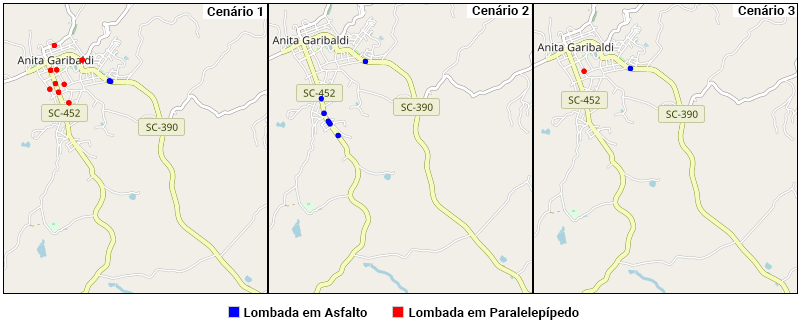
\includegraphics[width=1\textwidth]{figuras/fig_26.png}
   \fonte{Desenvolvido pelo autor.}
\end{figure}

\begin{table}[H]
\scriptsize
\centering
\caption{Métricas para as classes de dados de lombadas} 
\label{table:lombada_metricas}
\begin{tabular}{ccccccc}
\cmidrule(l){3-7}
\multicolumn{1}{l}{} & 
\multicolumn{1}{l}{} & 
\multicolumn{3}{c}{\textbf{Número de Amostras}} & 
\multicolumn{2}{c}{\textbf{Distribuição das Classes de Dados (\%)}} \\ \midrule
\textbf{Cenário} & 
\textbf{Conjunto} & 
\textbf{Com Lombada} & 
\textbf{Sem Lombada} & 
\textbf{Total} & 
\textbf{Com Lombada} & 
\textbf{Sem Lombada} \\ \midrule

\multirow{4}{*}{1} & PVS 1 & 3455 & 140581 & 144036 & 2.39 & 97.60 \\ \cmidrule(l){2-7} 
 & PVS 4 & 3134 & 129358 & 132492 & 2.37 & 97.63 \\ \cmidrule(l){2-7} 
 & PVS 7 & 2876 & 125672 & 128548 & 2.24 & 97.76 \\ \midrule
 
\multirow{4}{*}{2} & PVS 2 & 2006 & 122679 & 124685 & 1.61 & 98.39 \\ \cmidrule(l){2-7} 
 & PVS 5 & 1943 & 131934 & 133877 & 1.45 & 98.55 \\ \cmidrule(l){2-7} 
 & PVS 8 & 1837 & 121781 & 123618 & 1.49 & 98.51 \\ \midrule
 
\multirow{4}{*}{3} & PVS 3 & 609 & 105207 & 105816 & 0.57 & 99.42 \\ \cmidrule(l){2-7} 
 & PVS 6 & 606 & 95673 & 96279 & 0.63 & 99.37 \\ \cmidrule(l){2-7} 
 & PVS 9 & 643 & 90914 & 91557 & 0.71 & 99.30 \\ \bottomrule
\end{tabular}
\fonte{Desenvolvido pelo autor.}
\end{table}

Por fim, foram criados os rótulos para o nível de qualidade da superfície de pista. Para estas classes de dados, foram criados os rótulos \emph{boa} (good\_road), \emph{regular} (regular\_road) e \emph{ruim} (bad\_road). Ao contrário das classes anteriores, as classes de qualidade podem tornar-se subjetivas de acordo com o GT utilizado. Inúmeros estudos rotulam a qualidade com base na percepção de qualidade de um usuário ou através da quantificação de irregularidades e obstáculos presentes no segmento de pista. Contudo, utilizar GT de anotação humana através das metodologias descritas acima torna as classes subjetivas, com viés a percepção de quem rotulou. Logo, de forma a tratar este problema, desenvolvemos um GT de anotação automatizada por máquina, baseado na análise de vibração.

O processo de anotação de qualidade de superfície se inicia com a quantificação da irregularidade longitudinal dos segmentos analisados, baseado no cálculo de IRI de \cite{Li2018}. A irregularidade calculada corresponde ao conjunto de desvios da superfície em relação a um plano de referência. Sendo assim, partindo de um \textit{baseline} onde a variação dos sinais dos sensores inerciais é 0, caracterizando um segmento regular, quanto maior essa variação (vibração), mais irregular é a superfície. Para calcular a irregularidade, foi empregado RMS, a qual consiste de uma técnica estatística que mede a magnitude de uma variação, sendo especialmente útil quando os valores empregados alternam entre positivos e negativos, como é o caso dos sinais analisados. 

A utilização do RMS com os dados dos sensores inerciais fornece a magnitude da irregularidade da superfície com a influência dos fatores de dependência. Sendo assim, é necessário considerar a forma com que cada um dos fatores influencia o valor resultante. Desta forma, após seu cálculo, a magnitude da irregularidade (propriedade ambiental) é normalizada pela velocidade acumulada no segmento de dados (propriedade de condução) \cite{Li2018}. Em suma, nesta primeira etapa, através de uma janela deslizante de 500 amostras, com 250 amostras à direita e outras 250 à esquerda, os sinais são convolvidos aplicando sobre eles RMS normalizado pela velocidade acumulada no segmento. A equação abaixo detalha este cálculo, onde \emph{i} é o índice da primeira amostra da janela, \emph{j} o índice da última amostra, \emph{R} o RMS dos sinais dos sensores inerciais, e \emph{v} a velocidade.

\begin{center}
  \[
  \textit{Vibração} = \frac{(j - i + 1) \cdot R}{\sum_{x=i}^{j} v_x} \cdot 100
  \]
\end{center}

As características de vibração foram extraídas para cada um dos conjuntos PVS. Em seguida, estas características foram agrupadas de acordo com o modelo de veículo utilizado (propriedade veicular), onde no primeiro grupo ficaram as características dos PVS 1-3 (Volkswagen Saveiro), no segundo as dos PVS 4-6 (Fiat Bravo), e no terceiro as dos PVS 7-9 (Fiat Palio). Uma vez que os três cenários de coleta de dados contam com ambientes nos quais há segmentos nos três níveis de qualidade, e que cada um dos agrupamentos por veículo conta com dados dos três cenários, podemos concluir que necessariamente cada agrupamento possuí características de alto nível que representam segmentos com pista de qualidade boa, regular e ruim. Sendo assim, em seguida cada agrupamento por veículo foi empregado separadamente em um modelo KMC de 3 \textit{clusters}, os quais representam os níveis de qualidade, onde as características de vibração foram agrupadas de acordo com sua similaridade. Os agrupamentos obtidos através do modelo de KMC resultou nos rótulos das classes de níveis de qualidade ilustrados na \autoref{fig:qualidade_superficies_mapa}. Uma vez que a qualidade da superfície depende diretamente do pneu que a toca, foram produzidos separadamente rótulos para os sensores colocados no lado direito do veículo, assim como aqueles do lado esquerdo. A \autoref{table:qualidade_superficie_metricas} detalha as métricas dessas classes.  
 
\begin{figure}[h!]
  \centering
  \caption{Diferentes níveis de qualidade de superfície presentes nos cenários}
   \label{fig:qualidade_superficies_mapa}
   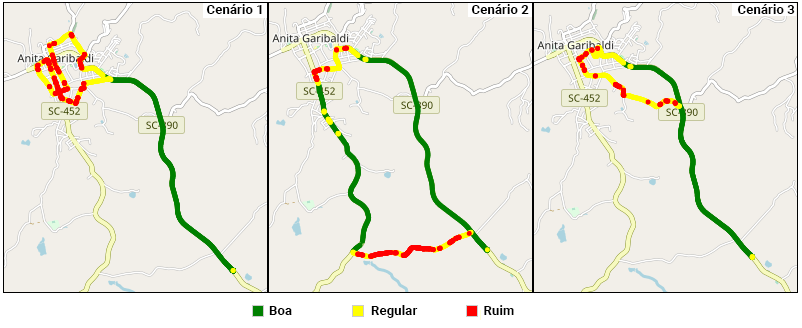
\includegraphics[width=1\textwidth]{figuras/fig_27.png}
   \fonte{Desenvolvido pelo autor.}
\end{figure}

\begin{table}[H]
\centering
\scriptsize
\caption{Métricas para as classes de dados de qualidade de superfície} 
\label{table:qualidade_superficie_metricas}
\begin{tabular}{clccccccc}
\cmidrule(l){3-9} & & 
\multicolumn{4}{c}{\textbf{Número de Amostras}} & 
\multicolumn{3}{c}{\textbf{Distribuição das Classes de Dados (\%)}} 
\\ \midrule

\multicolumn{1}{c}{\textbf{Cenário}} &
\textbf{Conjunto} &
\textbf{Boa} &
\textbf{Regular} &
\textbf{Ruim} & 
\textbf{Total} &
\textbf{Boa} &
\textbf{Regular} &
\textbf{Ruim}
\\ \midrule

\multicolumn{1}{c}
{\multirow{8}{*}{1}} & PVS 1 Esquerda &  56577 & 65304 & 22155 & 144036 & 39.28 & 45.34 & 15.38 \\ \cmidrule(l){2-9} 
\multicolumn{1}{c}{} & PVS 1 Direita & 56595 & 66038 & 21403 & 144036 & 39.29 & 45.85 & 14.86 \\ \cmidrule(l){2-9} 
\multicolumn{1}{c}{} & PVS 4 Esquerda & 50744 & 62838 & 18910 & 132492 & 38.30 & 47.43 & 14.27 \\ \cmidrule(l){2-9} 
\multicolumn{1}{c}{} & PVS 4 Direita & 50732 & 64102 & 17658 & 132492 & 38.29 & 48.38 & 13.33 \\ \cmidrule(l){2-9} 
\multicolumn{1}{c}{} & PVS 7 Esquerda & 49855 & 64743 & 13950 & 128548 & 38.78 & 50.36 & 10.85 \\ \cmidrule(l){2-9} 
\multicolumn{1}{c}{} & PVS 7 Direita & 50040 & 67230 & 11278 & 128548 & 38.93 & 52.30 & 8.77 \\ \midrule

\multicolumn{1}{c}
{\multirow{8}{*}{2}} & PVS 2 Esquerda & 56086 & 37921 & 30677 & 124684 & 44.98 & 30.41 & 24.60 \\ \cmidrule(l){2-9} 
\multicolumn{1}{c}{} & PVS 2 Direita & 55926 & 38057 & 30701 & 124684 & 44.85 & 30.52 & 24.62 \\ \cmidrule(l){2-9} 
\multicolumn{1}{c}{} & PVS 5 Esquerda & 53715 & 32999 & 47163 & 133877 & 40.12 & 24.65 & 35.23 \\ \cmidrule(l){2-9} 
\multicolumn{1}{c}{} & PVS 5 Direita & 53510 & 32587 & 47780 & 133877 & 39.97 & 24.34 & 35.69 \\ \cmidrule(l){2-9} 
\multicolumn{1}{c}{} & PVS 8 Esquerda & 56466 & 29949 & 37203 & 123618 & 45.68 & 24.23 & 30.10 \\ \cmidrule(l){2-9} 
\multicolumn{1}{c}{} & PVS 8 Direita & 56617 & 32301 & 34700 & 123618 & 45.80 & 26.13 & 28.07 \\ \midrule

\multicolumn{1}{c}
{\multirow{8}{*}{3}} & PVS 3 Esquerda & 50923 & 46638 & 8255 & 105816 & 48.12 & 44.07 & 7.80 \\ \cmidrule(l){2-9}
\multicolumn{1}{c}{} & PVS 3 Direita & 50906 & 47384 & 7526 & 105816 & 48.11 & 44.78 & 7.11 \\ \cmidrule(l){2-9} 
\multicolumn{1}{c}{} & PVS 6 Esquerda & 40446 & 51051 & 4782 & 96279 & 42.01 & 53.02 & 4.97 \\ \cmidrule(l){2-9} 
\multicolumn{1}{c}{} & PVS 6 Direita & 40453 & 50180 & 5646 & 96279 & 42.02 & 52.12 & 5.86 \\ \cmidrule(l){2-9} 
\multicolumn{1}{c}{} & PVS 9 Esquerda & 42557 & 38919 & 10079 & 91555 & 46.48 & 42.51 & 11.01 \\ \cmidrule(l){2-9} 
\multicolumn{1}{c}{} & PVS 9 Direita & 42711 & 42625 & 6219 & 91555 & 46.65 & 46.56 & 6.79 \\ \bottomrule

\end{tabular}
\fonte{Desenvolvido pelo autor.}
\end{table}

\chapter{Classificação de Tipo de Superfície de Pista 1}
\label{cap:classificacao_tipo_superficie_1}

Nesta seção é apresentado o primeiro de dois estudos voltados ao desenvolvimento de um modelo adaptativo para classificação do tipo da superfície de pista. Este estudo teve como objetivo experimentar e comparar modelos baseados em algumas das técnicas mais utilizadas nos estudos relacionados, com modelos baseados em \textit{Deep Learning}. O processo de desenvolvimento e experimentação é detalhado nas próximas subseções. Na primeira delas, o pré-processamento, foi realizada a seleção de variáveis, normalização dos sinais, extração de características e separação de dados para treinamento e validação. O \textit{design} experimental foi produzido de forma a construir experimentos que permitiram avaliar a capacidade de generalização do aprendizado de cada modelo para contextos desconhecidos e, portanto, avaliar sua adaptabilidade. Na segunda subseção, processamento, foram desenvolvidos e testados 34 diferentes modelos para classificar a superfície de pista, dentre modelos de Aprendizado de Máquina clássico e \textit{Deep Learning}. Por fim, na última subseção são detalhados e comparados os resultados obtidos. 

\section{Pré-Processamento}

Com os conjuntos de dados criados, os dados brutos foram pré-processados antes de serem entregues aos modelos de Aprendizado de Máquina. Este estudo teve como foco a utilização dos valores amostrados no braço de controle, localizado abaixo e próximo ao sistema de suspensão. De acordo com o modelo QC, esses valores possuem interferência apenas da massa não suspensa por meio da rigidez e absorção do pneu \cite{Yafeai2019}. Sendo assim, cada amostra utilizada possuí os valores de força de aceleração e de taxa de rotação, ambos em três eixos, e o valor da velocidade. Neste estudo, utilizamos de ambos os sensores inercias uma vez que os consideramos complementares, com cada um deles fornecendo um tipo específico de dado acerca dos movimentos veiculares. Também consideramos todos os eixos dos sensores e não apenas o de maior interesse, como geralmente é feito nos estudos de exterocepção, uma vez que todos os eixos apresentam informações relevantes, que devem ser consideradas no desenvolvimento de um modelo mais confiável.

Após a seleção das sete variáveis, seus dados foram transformados para se adequar às entradas das técnicas de classificação de padrões. Para os modelos de Aprendizado de Máquina clássicos, foi necessário extrair em pré-processamento as características de alto nível que bem representem as classes de dados. Para isto, foram aplicados os métodos estatísticos Desvio Padrão, Média e Variância para sinais de sensores inerciais e Média para velocidade, os quais constituem os métodos mais comumente usados em estudos relacionados para extrair características baseadas em vibração de sinais de sensores inerciais \cite{Alqudah2016,Andria2016,BelloSalau2018,Bose2018,Hou2017,Li2016,Lima2016,Pholprasit2015,Prapulla2017,Savera2016,Singh2017}. Para os modelos baseados em \textit{Deep Learning}, uma vez que estas técnicas produzem melhor desempenho quando as variáveis são escaladas em uma faixa de valores, os dados foram normalizados com \textit{Robust Scaler}, \textit{Min Max Scaler} no intervalo [0,1] e \textit{Min Max Scaler} no intervalo [-1,1]. Para analisar a influência do número de amostras em todos os modelos, foram criados os \emph{experimentos por tamanho de janela}, onde foram utilizadas janelas fixas de 100, 150, 200, 250 e 300 amostras, considerando 100 o tamanho mínimo para ter informação suficiente, e 300 o tamanho máximo para que o atraso da primeira classificação seja não superior a 3 segundos. 

Após a transformação dos dados, definiu-se quais foram utilizados para treinamento e para validação. Embora um mesmo conjunto de dados seja comumente dividido em uma parte para treinamento e outra para validação (geralmente 70\% - 30\%), ou os conjuntos de dados sejam aplicados em uma metodologia de validação cruzada \textit{k-fold}, ambas as abordagens no contexto deste estudo incorrem em viés por duas razões. A primeira, se todos os conjuntos de dados possuírem uma parte para treinamento e outra para validação ou sejam distribuídos na abordagem \textit{k-fold} de k igual a 9, isso implica que a técnica de reconhecimento de padrões terá para treinamento dados amostrados em todos os veículos, com todos os motoristas, e em todos os cenários. Isso, por si só, já leva a técnica a obter excelentes resultados, mas não nos diz nada sobre a capacidade de generalizar seu aprendizado de classificar padrões em contextos desconhecidos. A segunda razão decorre de que esse tipo de divisão pode levar a situações em que os dados de validação são compostos principalmente por dados com padrões mais facilmente reconhecidos, como segmentos de pavimento asfáltico, uma vez que a vibração do sinal neste tipo de superfície é muito menor do que nas outras. Portanto, para avaliar corretamente a generalização de cada técnica, avaliando sua confiabilidade em contextos desconhecidos (diferentes veículos, motoristas ou cenários/ambientes), os dados de treinamento e validação foram divididos de acordo com o conjunto de dados, separando-os em três \emph{experimentos por contexto}:

\begin{description}
	
	\item[Experimento por Contexto 1:] O modelo aprende dados de todos os veículos e motoristas para alguns cenários; mas não todos os veículos com todos os motoristas para todos os cenários.
    \begin{itemize}
        \item \textbf{Treinamento (65\%):} PVS 1, PVS 3, PVS 4, PVS 6, PVS 7, PVS 9. 
        \item \textbf{Validação (35\%):} PVS 2, PVS 5, PVS 8.
    \end{itemize}
    
    \item[Experimento por Contexto 2:] O modelo aprende dados de todos os cenários para alguns veículos e alguns motoristas; mas não todos os veículos com todos os motoristas para todos os cenários.
    \begin{itemize}
        \item \textbf{Treinamento (66\%):} PVS 1, PVS 2, PVS 3, PVS 7, PVS 8, PVS 9.
        \item \textbf{Validação (34\%):} PVS 4, PVS 5, PVS 6.
    \end{itemize}
    
    \item[Experimento por Contexto 3:] O modelo aprende dados de alguns veículos com alguns motoristas para alguns cenários; mas não todos os veículos com todos os motoristas para todos os cenários.
    \begin{itemize}
        \item \textbf{Treinamento (66\%):} PVS 1, PVS 2, PVS 4, PVS 6, PVS 8, PVS 9.
        \item \textbf{Validação (34\%):} PVS 3, PVS 5, PVS 7.
    \end{itemize}
    
\end{description}

É importante observar que cada conjunto de dados consiste em um conjunto disjunto de variáveis. Portanto, cada um deles contém dados para todas as variáveis de entrada do modelo (força de aceleração, taxa de rotação e velocidade) e a representação de todas as classes de dados (terra, paralelepípedo e asfalto). O que diferencia um conjunto de outro é o contexto de coleta de dados, onde há variação nas propriedades de dependência. A \autoref{fig:divisao_conjuntos_pvs} ilustra a divisão dos grupos de treinamento e validação de acordo com essas propriedades.

\begin{figure}[h]
  \centering
  \caption{Divisão dos conjuntos de dados PVS em grupos de treinamento e validação.}
  \label{fig:divisao_conjuntos_pvs}
  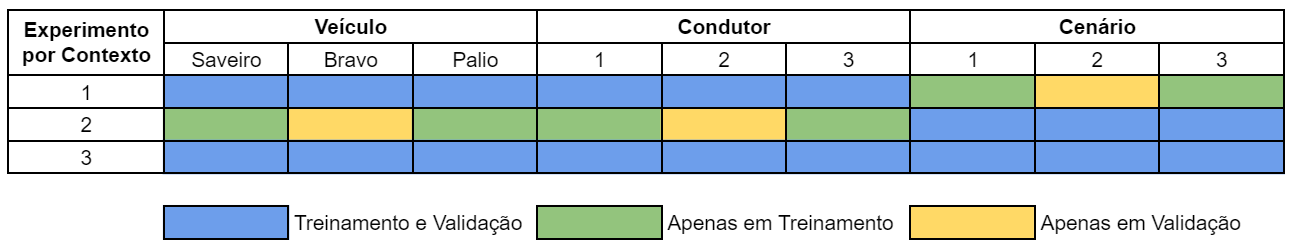
\includegraphics[width=1\textwidth]{figuras/fig_29.png}
  \fonte{Desenvolvido pelo autor.}
\end{figure}

Embora a abordagem de divisão de dados adotada não seja comum, ela foi necessária para permitir avaliar o comportamento dos modelos de Aprendizado de Máquina quando submetido a dados coletados em um veículo, motorista ou cenário desconhecido. Nos três experimentos, todas as classes de dados estão presentes na fase de treinamento e validação. Para avaliar a necessidade de aplicar técnicas de balanceamento de classe de dados, foi medido a distribuição de cada classe conforme detalhado na \autoref{table:distribuicao_classes_tipo_superficie}. A distribuição de classes foi calculada com os dados de treinamento \cite{He2013,Kuhn2013}, uma vez que estes são os dados utilizados pelos modelos para aprender os padrões. A distribuição foi calculada em relação ao número de amostras, uma vez que as janelas de dados são definidas de acordo com esse parâmetro.

\begin{table}[h]
\caption{Distribuição de classes de dados de tipo de superfície de pista.}
\label{table:distribuicao_classes_tipo_superficie}
\centering
\scriptsize
\begin{tabular}{lcccccc}
\cmidrule(l){2-7}
\multicolumn{1}{c}{\multirow{2}{*}{\textbf{}}} & 
\multicolumn{6}{c}{\textbf{Classe de Dados}} \\ \cmidrule(l){2-7} 
\multicolumn{1}{c}{} & 
\multicolumn{2}{c}{\textbf{Terra}} & 
\multicolumn{2}{c}{\textbf{Paralelepípedo}} & 
\multicolumn{2}{c}{\textbf{Asfalto}} \\ \midrule
\textbf{Fonte de Dados} & 
\textit{\textbf{Percentual}} & 
\textit{\textbf{Proporção}} & 
\textit{\textbf{Percentual}} & 
\textit{\textbf{Proporção}} & 
\textit{\textbf{Percentual}} & 
\textit{\textbf{Proporção}} \\ \midrule
Todos os Conjuntos & 27.69\% & 1:2.6 & 29.07\% & 1:2.4 & 43.23\% & 1:1.3 \\ \midrule
Exp. por Contexto 1 & 21.36\% & 1:3.7 & 36.71\% & 1:1.7 & 41.92\% & 1:1.4 \\ \midrule
Exp. por Contexto 2 & 26.59\% & 1:2.8 & 28.78\% & 1:2.5 & 44.61\% & 1:1.2 \\ \midrule
Exp. por Contexto 3 & 26.15\% & 1:2.8 & 30.26\% & 1:2.3 & 43.58\% & 1:1.3 \\ \bottomrule
\end{tabular}
\fonte{Desenvolvido pelo autor.}
\end{table}

Analisando a \autoref{table:distribuicao_classes_tipo_superficie}, observamos que a distribuição das classes de tipo de superfície de pista situa-se entre 21.36\% e 44.61\%, dependendo do experimento. A proporção varia entre 1:1.2 a 1:3.7, onde para 1 amostra de uma determinada classe de dados, existem de 1.2 a 3.7 amostras nas outras classes. De acordo com \cite{Fernandez2018}, um conjunto de dados é considerado desbalanceado quando existe uma desproporção significativa, ou em alguns casos severa, entre o número de amostras de cada classe. O desbalanceamento de classes pode ser considerado leve ou severo, onde as proporções de distribuição que variam de 1:4 até 1:100 (presença de 20\% - 1\%) são consideradas desbalanceamento leve e proporções de distribuição que variam de 1:100 ou mais (<1\% de presença) são consideradas desbalanceamentos severos \cite{Krawczyk2016,Brownlee2020}. Como podemos observar, as proporções de distribuição das classes de dados neste estudo não é classificada sequer como desbalanceamento leve, pois em seu pior caso, a proporção 1:3.7 ainda é uma distribuição mais uniforme do que 1:4. De acordo com \cite{Brownlee2020}, o desbalanceamento leve geralmente não é uma preocupação, e o problema pode ser tratado como um problema de modelagem preditiva ou classificação normal. Sendo assim, se desbalanceamentos leves não dependem de balanceamento de classes, distribuições mais uniformes, como é o caso deste estudo, certamente não necessitam de aplicação desta técnica.

\section{Processamento}

Após a etapa de pré-processamento, os dados foram utilizados em técnicas de Inteligência Artificial para classificação do tipo de superfície de pista. Por meio de nossa RSL sobre percepção veicular, identificamos as principais técnicas utilizadas na exterocepção veicular com sensores inerciais, a qual tem como objetivo reconhecer as características do ambiente externo como tipo de superfície, qualidade do pavimento, buracos, lombadas, etc. Todos os modelos de Aprendizado de Máquina empregados em estudos anteriores na área são baseados em técnicas clássicas. Portanto, neste estudo foi realizada uma comparação entre as técnicas mais utilizadas na área, todas elas sendo o Aprendizado de Máquina clássico, com as técnicas de Aprendizado Profundo (\textit{Deep Learning}), as quais ainda não foram utilizadas neste tipo de problema de classificação.

Dentre as técnicas de Aprendizado de Máquina clássico mais aplicadas na área, estão as três experimentadas neste estudo: KMC, SVM e KNN. Para a técnica de KMC, foram desenvolvidos modelos com 3 \textit{clusters}, representando as classes a serem agrupadas. Para a técnica de SVM, foram experimentados modelos com três diferentes \textit{kernels}: polinomial de grau 3, rbf e sigmoid. Por fim, para a técnica de KNN, de forma a identificar o valor ótimo de vizinhos, foram desenvolvidos modelos com 1, 2, 5, 10, 50, 100, 250, 500, 1000 vizinhos. No desenvolvimento dos modelos de \textit{Deep Learning}, uma vez que nenhum estudo de exterocepção aplica este tipo de técnica, os modelos produzidos foram baseados em modelos de outros domínios que também utilizam de sensores inerciais para reconhecer padrões. Sendo assim, as Redes Neurais Profundas (\textit{Deep Neural Networks - DNN}) desenvolvidas foram baseadas em estudos de reconhecimento de atividade humana \cite{Deep2019,Alemayoh2019,Chen2015,Yang2018,Zebin2018,Zebin2019,Wang2019,Ahmad2019}, estimativa de velocidade de caminhada \cite{Shrestha2018} e classificação de terrenos durante corrida humana \cite{Dixon2019}. Foram construídos e analisados modelos baseados em LSTM, CNN e CNN-LSTM. Todos os modelos de DNN utilizam o otimizador Adam em conjunto com a função de perda de Entropia Cruzada Categórica, uma vez que se trata de um problema de classificação multi-classe.

Para as redes baseadas em LSTM, vários modelos foram desenvolvidos, dentre \textit{Vanilla} LSTM e \textit{Stacked} LSTM, tanto na forma unidirecional quanto bidirecional, detalhados na \autoref{table:lstm_superficie_pista_1}. O LSTM 7 foi o modelo desenvolvido com melhores resultados, consistindo de uma LSTM \textit{Stacked} Unidirecional detalhada na \autoref{fig:best_lstm_tipo_superficie_1}. Neste modelo, a DNN recebe um tensor de entrada \emph{janelas x sequências x características}, onde \emph{janelas} são os agrupamentos de janelas, \emph{sequências} são os dados que uma janela possui, ou seja, a sequencia de amostras, e \emph{características} são os valores das 7 variáveis dos sensores, sendo assim, os valores de cada amostra. O modelo é composto por uma camada de entrada, três blocos de recorrência e regularização, e um bloco de camadas totalmente conectadas para produção de saída. As camadas de LSTM com 100 unidades são utilizadas para aprender as dependências temporais de longo prazo na sequência de dados. A regularização é feita por duas camadas, sendo \textit{Batch Normalization} para padronizar as entradas de uma nova camada, reduzindo o tempo de treinamento e melhorando o desempenho \cite{Zebin2018}; e \textit{Dropout} em 50\% para evitar \textit{overfitting}, ignorando neurônios selecionados aleatoriamente durante o treinamento. Após o processamento nas camadas recorrentes, os parâmetros são passados para duas camadas \textit{Dense}, a primeira com 100 neurônios com ativação Relu, e a segunda com 3 neurônios e ativação do Softmax, produzindo a classificação. A saída esperada da rede são os rótulos correspondentes à última amostra da janela.

\begin{center}
\scriptsize
\begin{longtable}{cl}
\caption{Modelos de LSTM para classificação do tipo de superfície de pista.}
\label{table:lstm_superficie_pista_1} \\
\toprule 
\multicolumn{1}{l}{\textbf{Nome}} & 
\multicolumn{1}{c}{\textbf{Camadas}} \\ \midrule
\endfirsthead
\toprule 
\multicolumn{1}{l}{\textbf{Nome}} & 
\multicolumn{1}{c}{\textbf{Camadas}} \\ \midrule
\endhead \endfoot \endlastfoot
LSTM 1 & 1 LSTM com 100 unidades, 1 Dropout de 0.5, 1 Dense com 100 unidades e ativação Relu,  1 Dense com 3 \\ & unidades e  ativação Softmax. \\ \midrule
LSTM 2 & Igual a LSTM 1, mas conetando as sequencias \textit{flattened} retornadas pela LSTM diretamente na camada Dense. \\ \midrule
LSTM 3 & Igual a LSTM 1, mas com LSTM bidirecional. \\ \midrule
LSTM 4 & Igual a LSTM 2, mas com LSTM bidirecional. \\ \midrule
LSTM 5 & 3 blocos de LSTM com 100 unidades e Dropout em 0.5, 1 Dense com 100 unidades e ativação Relu, 1 Dense \\ & com 3  unidades e ativação Softmax.\\ \midrule
LSTM 6 & Igual a LSTM 5, mas com LSTM bidirecional e Dropout em 0.2 \\ \midrule
LSTM 7 & 3 blocos de LSTM com 100 unidades, Batch Normalization e Dropout 0.5, 1 Dense com 100 unidades e \\ & ativação Relu, 1 Dense com 3 unidades e ativação Softmax. \\ \bottomrule
\end{longtable}
\fonte{Desenvolvido pelo autor.}
\end{center}

\begin{figure}[h]
  \centering
  \caption{Melhor modelo de LSTM para classificação de superfície de pista.}
  \label{fig:best_lstm_tipo_superficie_1}
  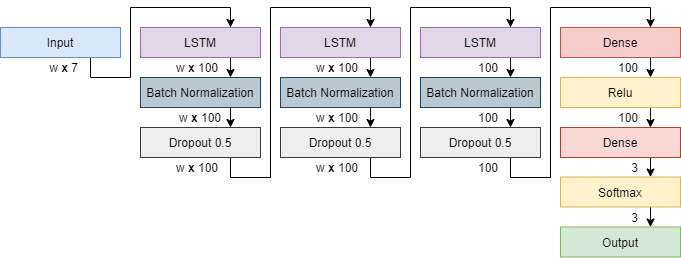
\includegraphics[width=0.8\textwidth]{figuras/fig_31.png}
  \fonte{Desenvolvido pelo autor.}
\end{figure}

Para as redes baseadas em CNN, foram produzidos modelos de CNN \textit{Stacked} utilizando de diferentes camadas de \textit{pooling}, conforme detalha a \autoref{table:cnn_superficie_pista_1}. O modelo desenvolvido com melhores resultados foi o CNN 8, detalhado na \autoref{fig:best_cnn_dnn_tipo_superficie_1}. Esta DNN recebe um tensor de entrada \emph{janelas x sequências x características} semelhante ao das redes baseadas em LSTM, o qual é processado por três blocos de camadas de convolução e regularização, e um bloco de camadas totalmente conectadas. Os blocos de extração de características utilizam nos sinais \textit{kernels} de convolução de tamanho 3, com a primeira camada possuindo 64 filtros e as demais com 32 filtros. A regularização é feita pelas camadas \textit{Batch Normalization} e \textit{Dropout} em 15\% e 20\%. O último bloco de extração de características também possui uma camada \textit{Global Average Pooling 1D} para extrair características mais robustas por valores médios em cada região, acelerando o processo de treinamento e evitando \textit{overfitting} \cite{Yang2018, Wang2019}. Por fim, o último bloco consiste de duas camadas \textit{Dense}, uma com 32 neurônios e ativação de Relu, e a outra com 3 neurônios e ativação de Softmax. A saída esperada da rede são os rótulos mais presentes na janela analisada.

\begin{center}
\scriptsize
\begin{longtable}{cl}
\caption{Modelos de CNN para classificação do tipo de superfície de pista.} 
\label{table:cnn_superficie_pista_1}  \\
\toprule \textbf{Nome} & \multicolumn{1}{c}{\textbf{Camadas}} \\ \midrule
\endfirsthead
\toprule \textbf{Nome} & \multicolumn{1}{c}{\textbf{Camadas}} \\ \midrule
\endhead \endfoot \endlastfoot
CNN 1 &
3 blocos de Conv1D com 64-64-128 filtros, \textit{kernel} de tamanho 3 e ativação Relu, 1 Flatten, 1 Dense com 100 \\ & unidades e ativação Relu, 1 Dense com 3 unidades e ativação Softmax. \\ \midrule
CNN 2 & Igual a CNN 1, mas com 1 Max Pooling 1D com \textit{pool} de tamanho 2 depois dos blocos de convolução. \\ \midrule
CNN 3 & 1 Conv1D com 64 filtros,  \textit{kernel} de tamanho 3 e ativação Relu, 1 Batch Normalization, 1 Dropout em 0.15, \\ & 1 Conv1D com 32 filtros, \textit{kernel} de tamanho 3 e ativação Relu, 1 Global Avg Pool 1D, 1 Batch Normalization, \\ & 1 Dropout 0.2 e 1 Dense com 3 unidades e ativação Softmax.
 \\ \midrule
CNN 4 & 2 Conv1D com 100 filtros, \textit{kernel} de tamanho 10 e ativação Relu, 1 Max Pooling 1D com \textit{pool} de tamanho 3, \\ & 2 Conv1D com 160 filtros, \textit{kernel} de tamanho 10 e ativação Relu, 1 Global Avg Pool 1D, 1 Dropout 0.5 e 1 Dense \\ & com 3 unidades e ativação Softmax.
 \\ \midrule
CNN 5 & 1 Conv1D com 64 filtros, \textit{kernel} de tamanho 3 e ativação Relu, 1 Max Pooling 1D com \textit{pool} de tamanho 2, 1 \\ & Conv1D com 64 filtros, \textit{kernel} de tamanho 3 e ativação Relu, 1 Flatten e 1 Dense com 3 unidades e ativação Softmax.
 \\ \midrule
CNN 6 & 1 Conv1D com 24 filtros, \textit{kernel} de tamanho 8 e ativação Relu, 1 Batch Normalization, 1 Spatial Dropout 0.15, 1 \\ & Conv1D com 12 filtros, \textit{kernel} de tamanho 8 e ativação Relu, 1 Global Avg Pool 1D, 1 Batch Normalization, \\ & 1 Dropout 0.2, 1 Dense com 48 unidades e ativação Relu, 1 Batch Normalization, 1 Dropout em 0.25, 1 Dense com \\ & 3 unidades e ativação Softmax. \\ \midrule
CNN 7 &  3 blocos de Conv1D com 128-64-32 filtros, \textit{kernel} de tamanho 3 e ativação Relu, 1 Batch Normalization e 1 \\ & Max Pooling 1D com \textit{pool} de tamanho 2, 1 Flatten, 1 Dropout em 0.2, 1 Dense com 3 unidades e ativação Softmax. \\ \midrule
CNN 8 & 2 blocos de Conv1D com 64-32 filtros, \textit{kernel} de tamanho 3 e ativação Relu, 1 Batch Normalization e 1 Dropout \\ & em 0.15, 1 Conv1D 32 filtros, \textit{kernel} de tamanho 3 e ativação Relu, 1 Global Avg Pool 1D, 1 Batch Normalization, \\ & 1 Dropout em 0.2, 1 Dense com 32 unidades e ativação Relu e 1 Dense com 3 unidades e ativação Softmax. \\ \bottomrule
\end{longtable}
\fonte{Desenvolvido pelo autor.}
\end{center}

\begin{figure}[H]
  \centering
  \caption{Melhor modelo de CNN para classificação do tipo de superfície de pista.}
  \label{fig:best_cnn_dnn_tipo_superficie_1}
  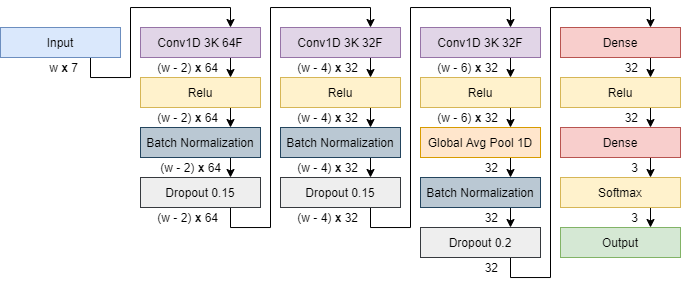
\includegraphics[width=0.8\textwidth]{figuras/fig_32.png}
  \fonte{Desenvolvido pelo autor.}
\end{figure}

Para as redes baseadas em CNN-LSTM, foram produzidos modelos híbridos detalhados na \autoref{table:cnn_lstm_superficie_pista_1}. O modelo desenvolvido com melhores resultados foi o CNN-LSTM 6, detalhado na \autoref{fig:best_cnn_lstm_tipo_superficie_1}. Esta DNN recebe um tensor \emph{janelas x sequências x subsequências x características}, onde \emph{janelas} são os agrupamentos de janelas, \emph{sequências} são as janelas de dados, \emph{subsequências} são os subgrupos de janelas e \emph{características} são os valores das 7 variáveis dos sensores. Os dados são inicialmente processados por três blocos de camadas de convolução e regularização, três blocos de camadas recorrentes e de regularização, e um bloco de camadas totalmente conectadas. Os blocos de extração de características utilizam nos sinais \textit{kernels} de convolução de tamanho 3 com 128 filtros. A regularização é feita pelas camadas de \textit{Batch Normalization} e \textit{Spatial Dropout 1D} em 15\% e 20\%. O último bloco possuí uma camada \textit{Global Average Pooling 1D}. Os blocos recorrentes possuem camadas de LSTM com 100 unidades e regularização por \textit{Batch Normalization} e \textit{Dropout} em 50\%. Finalmente, os parâmetros resultantes são entregues a uma camada \textit{Dense} com 3 neurônios e ativação do Softmax, produzindo a classificação. A saída esperada da rede são os rótulos correspondentes à última amostra na janela.

\begin{center}
\scriptsize
\begin{longtable}{cl}
\caption{Modelos de CNN-LSTM para classificação do tipo de superfície de pista.} 
\label{table:cnn_lstm_superficie_pista_1} \\
\toprule \textbf{Nome} & \multicolumn{1}{c}{\textbf{Camadas}} \\ \midrule
\endfirsthead
\toprule \textbf{Nome} & \multicolumn{1}{c}{\textbf{Camadas}} \\ \midrule
\endhead \endfoot \endlastfoot
CNN-LSTM 1 &  2 Conv1D com 64 filtros, \textit{kernel} de tamanho 3 e ativação Relu, 1 Dropout em 0.5, 1 Max Pooling 1D \\ & com \textit{pool} de tamanho 2, 1 Flatten, 1 LSTM com 100 unidades, 1 Dropout em 0.2, 1 Dense com 100 \\ & unidades e ativação Relu, 1 Dense com 3 unidades e ativação Softmax. \\ \midrule
CNN-LSTM 2 & Igual a CNN-LSTM 1, mas com 3 camadas Conv1D. \\ \midrule
CNN-LSTM 3 & Igual a CNN-LSTM 2, mas com 3 blocos de LSTM e Dropout após a camada Max Pooling 1D. \\ \midrule
CNN-LSTM 4 & Igual a CNN-LSTM 3, mas com os blocos LSTM sem camada Dropout. \\ \midrule
CNN-LSTM 5 &  2 blocos de Conv1D com 128 filtros, \textit{kernel} de tamanho 3 e ativação Relu, Max Pooling 1D com \textit{pool} \\ & de tamanho 2 e Batch Normalization, 1 bloco de 1 Conv1D com 128 filtros, \textit{kernel} de tamanho 3 e ativação \\ & Relu,  Global Avg Pool 1D e Batch Normalization, 3 blocos de 1 LSTM com 100 unidades, Batch \\ & Normalization e Dropout em 0.3, 1 Dense com 3 unidades e ativação Softmax. \\ \midrule
CNN-LSTM 6 & 2 blocos de 1 Conv1D com 128 filtros, \textit{kernel} de tamanho 3 e ativação Relu, Batch Normalization, e Spatial \\ &  Dropout em 0.15, 1 bloco de Conv1D com 128 filtros, \textit{kernel} de tamanho 3 e ativação Relu, Global Avg Pool \\& 1D, Batch Normalization e Dropout em 0.2, 3 blocos de LSTM com 100 unidades, Batch Normalization e \\ & Dropout em 0.3, 1 Dense com 3 unidades e ativação Softmax. \\ \bottomrule
\end{longtable}
\fonte{Desenvolvido pelo autor.}
\end{center}

\begin{figure}[h]
  \centering
  \caption{Melhor modelo de LSTM-CNN para classificação do tipo de superfície de pista.}
  \label{fig:best_cnn_lstm_tipo_superficie_1}
  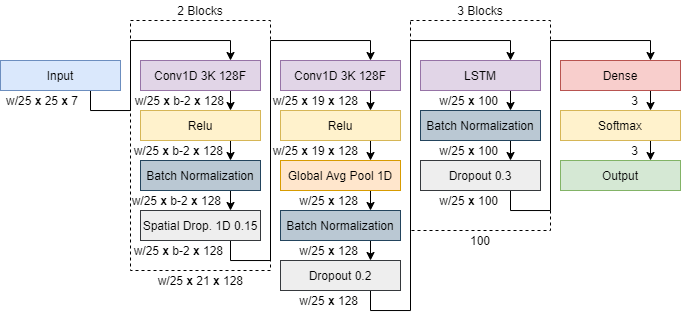
\includegraphics[width=0.8\textwidth]{figuras/fig_33.png}
 \fonte{Desenvolvido pelo autor.}
\end{figure}

\section{Análise de Resultados}

Todos os modelos desenvolvidos neste estudo foram programados em Python 3. Os modelos Aprendizado de Máquina clássico usaram a biblioteca Scikit-Learn, enquanto os modelos \textit{Deep Learning} utilizaram o \textit{framework} Keras com o \textit{backend} Tensorflow. Os experimentos foram realizados no Google Collaboratory, com uma GPU NVIDIA Tesla P100 com 12 GB e 25 GB de RAM. Em todas as técnicas, exceto KNN, os experimentos foram executados 3 vezes a fim de minimizar a aleatoriedade dos parâmetros iniciais, recuperando apenas o melhor entre os três. Cada experimento consiste de um elemento do produto cartesiano entre \emph{experimentos por tamanho de janela} e \emph{experimentos por contexto}. Os resultados obtidos na aplicação do Aprendizado de Máquina clássico são detalhados nas Tabelas \ref{table:kmc_results_tipo_superficie_1}, \ref{table:svm_results_tipo_superficie_1} e \ref{table:knn_results_tipo_superficie_1}. O valor detalhado corresponde à média de acurácia em  validação dos três \textit{experimentos por contexto} para um determinado \emph{experimento por tamanho de janela} e configuração dos hiper-parâmetros da técnica.

\begin{table}[H]
\scriptsize
\centering
\caption{Média de acurácia em validação para os modelos de KMC.} 
\label{table:kmc_results_tipo_superficie_1}
\begin{tabular}{ccccccc}
\cmidrule(lr){2-6}
& \multicolumn{5}{c}{\textbf{Experimentos por Tamanho de Janela}} & \multicolumn{1}{c}{} \\ \midrule
\textbf{Clusters} & \textbf{100} & \textbf{150} & \textbf{200} & \textbf{250} & \textbf{300} & \textbf{Média} \\ \midrule
3 & 56.20\% & 58.13\% &  59.10\% & 59.67\% & \cellcolor[HTML]{34FF34}\textbf{60.42\%} & 58.70\% \\ \bottomrule
\end{tabular}
\fonte{Desenvolvido pelo autor.}
\end{table}

\begin{table}[H]
\scriptsize
\centering
\caption{Média de acurácia em validação para os modelos de SVM.} 
\label{table:svm_results_tipo_superficie_1}
\begin{tabular}{ccccccc}
\cmidrule(lr){2-6}
& \multicolumn{5}{c}{\textbf{Experimentos por Tamanho de Janela}} & \multicolumn{1}{c}{} \\ \midrule
\textbf{Kernel} & \textbf{100} & \textbf{150} & \textbf{200} & \textbf{250} & \textbf{300} & \textbf{Média} \\ \midrule
poly 3 & 65.00\% & 66.60\% & 68.05\% & 68.07\% & \textbf{68.71\%} & 67.28\% \\ \midrule
rbf & 71.95\% & 72.28\% & \cellcolor[HTML]{34FF34}\textbf{72.68\%} & 72.42\% & 72.45\% & 72.36\% \\ \midrule
sigmoid & 52.80\% & 47.08\% & \textbf{57.50\%} & 54.73\% & 56.75\% & 53.77\% \\ \midrule
\textbf{Média} & 63.25\% & 61.99\% & 66.08\% & 65.08\% & 65.97\% & 64.47\% \\ \bottomrule
\end{tabular}
\fonte{Desenvolvido pelo autor.}
\end{table}

\begin{table}[H]
\scriptsize
\centering
\caption{Média de acurácia em validação para os modelos de KNN.} 
\label{table:knn_results_tipo_superficie_1}
\begin{tabular}{ccccccc}
\cmidrule(lr){2-6}
& \multicolumn{5}{c}{\textbf{Experimentos por Tamanho de Janela}} & \multicolumn{1}{c}{} \\ \midrule
\textbf{Vizinhos} & \textbf{100} & \textbf{150} & \textbf{200} & \textbf{250} & \textbf{300} & \textbf{Média} \\ \midrule
1 & 72.28\% & 72.77\% & \textbf{74.46\%} & 73.45\% & 73.83\% & 73.36\% \\ \midrule
2 & 59.80\% & 61.08\% & \textbf{62.69\%} & 60.87\% & 61.92\% & 61.27\% \\ \midrule
5 & 72.37\% & 72.78\% & \cellcolor[HTML]{34FF34}\textbf{74.79\%} & 73.80\% & 73.97\% & 73.54\% \\ \midrule
10 & 67.97\% & 68.39\% & \textbf{70.23\%} & 68.81\% & 69.72\% & 69.02\% \\ \midrule
50 & 70.83\% & 71.54\% & \textbf{72.01\%} & 71.30\% & 69.66\% & 71.07\% \\ \midrule
100 & 69.40\% & \textbf{69.75\%} & 69.47\% & 68.77\% & 67.63\% & 69.00\% \\ \midrule
250 & \textbf{66.25\%} & 65.18\% & 63.84\% & 62.61\% & 61.24\% & 63.83\%\\ \midrule
500 & \textbf{62.15\%} & 59.57\% & 57.66\% & 54.65\% & 53.93\% & 57.59\% \\ \midrule
1000 & \textbf{54.93\%} & 51.42\% & 49.12\% & 45.83\% & 44.05\% & 49.07\% \\ \midrule
\textbf{Média} & 66.22\% & 65.83\% & 66.03\% & 64.45\% & 63.99\% & 65.31\% \\ \bottomrule
\end{tabular}
\fonte{Desenvolvido pelo autor.}
\end{table}

Para a técnica KMC, o melhor modelo resultante para 3 \textit{clusters} foi o de janela com 300 amostras, atingindo 58.24\% de acurácia em treinamento e 60.42\% em validação. Nessa técnica, quanto maior a janela de dados aplicada, maiores os valores de acurácia obtidos. Na técnica SVM, o \textit{kernel} sigmoid obteve os piores valores de acurácia para todas as janelas de dados, seguido pelo \textit{kernel} polinomial de grau 3. Sendo assim, o \textit{kernel} rbf obteve os melhores valores de acurácia para todas as variações de tamanho de janela, onde o modelo com 200 amostras obteve acurácia de 76.15\% para treinamento e 72.68\% para validação. Neste \textit{kernel}, o tamanho da janela de dados tem pouca influência no resultado final. Por fim, os modelos de KNN apresentaram melhores resultados com o número de vizinhos entre 1-50, onde o tamanho da janela também não tem muita influência no resultado. Com grande número de vizinhos, os resultados tendem a apresentar uma variação maior de acordo com o número de amostras na janela. Para o número de vizinhos entre 1-50, a janela com 200 amostras apresentou os melhores resultados, situando o melhor modelo com 5 vizinhos, onde obteve acurácia no conjunto de dados de treinamento de 85.90\% e 74.79\% na validação. Com esses resultados, os melhores modelos de cada técnica clássica são detalhados na \autoref{table:classical_ml_results_tipo_superficie_1}, separados por \emph{experimento por contexto}.

\begin{table}[H]
\scriptsize
\centering
\caption{Valores de acurácia para os melhores modelos baseados em técnicas clássicas de aprendizado de máquina.} 
\label{table:classical_ml_results_tipo_superficie_1}
\begin{tabular}{clcccc}
\cmidrule(lr){3-5}
& & \multicolumn{3}{c}{\textbf{Experimentos por Contexto}} & \multicolumn{1}{c}{} \\ \midrule
\textbf{Modelo} & \multicolumn{1}{c}{\textbf{Fase}} & \textbf{1} & \textbf{2} & \textbf{3} & \textbf{Média} \\ \midrule
\multirow{2}{*}{KMC} & Treinamento & 60.53\% & 56.04\% & 58.13\% & 58.24\% \\ \cmidrule(l){2-6} 
 & Validação & 65.67\% & 60.32\% & 55.26\% & 60.42\% \\ \midrule
\multirow{2}{*}{SVM} & Treinamento & 75.59\% & 77.03\% & 75.84\% & 76.15\% \\ \cmidrule(l){2-6} 
 & Validação & 67.28\% & 75.61\% & 75.16\% & 72.68\% \\ \midrule
\multirow{2}{*}{KNN} & Treinamento & 84.50\% & 86.44\% & 86.76\% & 85.90\% \\ \cmidrule(l){2-6} 
 & Validação & 76.28\% & 71.11\% & 76.98\% & \cellcolor[HTML]{34FF34}\textbf{74.79\%} \\ \bottomrule
\end{tabular}
\fonte{Desenvolvido pelo autor.}
\end{table}

Observando os resultados da Tabela \ref{table:classical_ml_results_tipo_superficie_1}, é possível perceber que a técnica de KNN não somente apresenta a maior média de acurácia, como também é a técnica mais estável, com menor variação de resultado entre experimentos com diferentes contextos. O KMC apresenta variância de 18.07\%, o SVM de 14.63\%, e o KNN de 6.85\%. Além disso, observando a matriz confusão dos melhores modelos na \autoref{fig:confusion_matrix_classical_tipo_superficie_1}, a KNN é a única técnica em que o melhor modelo possuí mais VP e VN que FP e FN, quando considerado cada tipo de superfície separadamente. Sendo assim, conforme detalhado na \autoref{table:classical_ml_metrics_tipo_superficie_1}, KNN tem os melhores valores para f1-score para duas das três classes de dados, classificando segmentos de terra com f1-score de 65.39\%, paralelepípedos com 53.65\% e asfalto com 95.97\%. 

\begin{figure}[H]
  \centering
  \caption{Matriz de confusão para cada melhor modelo de técnicas clássicas de aprendizado de máquina.}
  \label{fig:confusion_matrix_classical_tipo_superficie_1}
  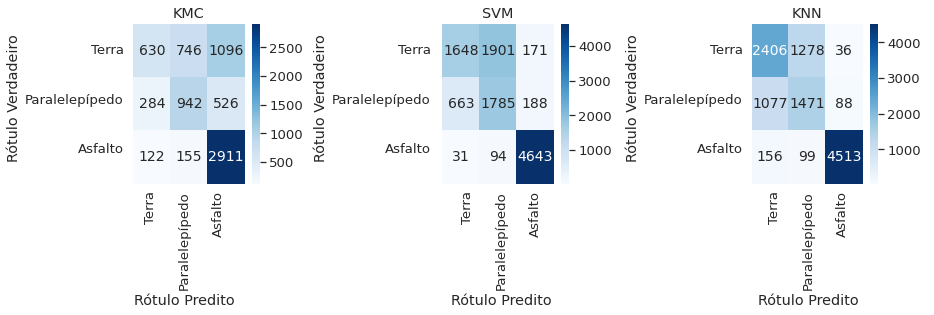
\includegraphics[width=1\textwidth]{figuras/fig_34.png}
  \fonte{Desenvolvido pelo autor.}
\end{figure}

\begin{table}[H]
\scriptsize
\centering
\caption{Métricas de avaliação para cada melhor modelo baseado em técnicas clássicas de aprendizado de máquina.} 
\label{table:classical_ml_metrics_tipo_superficie_1}
\begin{tabular}{clccc}
\toprule
\textbf{Modelo} & \multicolumn{1}{c}{\textbf{Classe de Dados}} & \textbf{F1-Score} & \textbf{Precisão} & \textbf{Recall} \\ \midrule
\multirow{4}{*}{KMC} & Asfalto & 75.40\% & 64.22\% & 91.31\% \\ \cmidrule(l){2-5} 
 & Paralelepípedo & 52.41\% & 51.11\% & 53.77\% \\ \cmidrule(l){2-5} 
 & Terra & 35.92\% & 60.81\% & 25.49\% \\ \midrule
\multirow{4}{*}{SVM} & Asfalto & 95.05\% & 92.82\% & 97.38\% \\ \cmidrule(l){2-5} 
 & Paralelepípedo & 55.64\% & 47.22\% & 67.71\% \\ \cmidrule(l){2-5} 
 & Terra & 54.37\% & 70.37\% & 44.30\% \\ \midrule
\multirow{4}{*}{KNN} & Asfalto & 95.97\% & 97.33\% & 94.65\% \\ \cmidrule(l){2-5} 
 & Paralelepípedo & 53.65\% & 51.65\% & 55.80\% \\ \cmidrule(l){2-5} 
 & Terra & 65.39\% & 66.12\% & 64.68\% \\ \bottomrule
\end{tabular}
\fonte{Desenvolvido pelo autor.}
\end{table}

Para os experimentos com as técnicas de \textit{Deep Learning}, inicialmente foram avaliados os diferentes métodos para normalização dos sinais. Dentre os três experimentados, o \textit{Min Max Scaler} entre [0,1] apresentou piores resultados, atingindo um maior valor de perda e uma acurácia menor. O \textit{Robust Scaler} foi o segundo melhor, mantendo o sinal nos dados, mas sem escalar em um intervalo fixo. Por fim, os dados normalizados com \textit{Min Max Scaler} entre [-1,1], mantendo o sinal e escalando em um intervalo fixo, apresentaram convergência mais rápida, menor perda e maior acurácia. Sendo assim, os escaladores que mantêm o sinal obtiveram melhores resultados, uma vez que o sinal é importante neste estudo, indicando a informação de direção e não apenas uma diminuição de valor. Utilizando os dados normalizados, foram experimentados os modelos de redes propostos. Os resultados são detalhados nas Tabelas \ref{table:lstm_results_tipo_superficie_1}, \ref{table:cnn_results_tipo_superficie_1} e \ref{table:cnn_lstm_results_tipo_superficie_1}.

\begin{table}[H]
\scriptsize
\centering
\caption{Média de acurácia em validação para redes baseadas em LSTM.} 
\label{table:lstm_results_tipo_superficie_1}
\begin{tabular}{ccccccc}
\cmidrule(lr){2-6}
& \multicolumn{5}{c}{\textbf{Experimentos por Tamanho de Janela}} & \multicolumn{1}{c}{} \\ \midrule
\textbf{Modelo} & \multicolumn{1}{c}{\textbf{100}} & \multicolumn{1}{c}{\textbf{150}} & \multicolumn{1}{c}{\textbf{200}} & \multicolumn{1}{c}{\textbf{250}} & \multicolumn{1}{c}{\textbf{300}} & \multicolumn{1}{c}{\textbf{Média}} \\ \midrule
LSTM 1 & 89.14\% & 89.44\% & \textbf{89.86\%} & 86.30\% & 87.59\% & 88.47\% \\ \midrule
LSTM 2 & \textbf{87.38\%} & 87.33\% & 86.80\% & 86.26\% & 85.85\% & 86.72\% \\ \midrule
LSTM 3 & 89.11\% & 89.61\% & 89.99\% & 89.21\% & \textbf{90.45\%} & 89.67\% \\ \midrule
LSTM 4 & 87.12\% & \textbf{87.31\%} & 87.07\% & 86.11\% & 86.48\% & 86.82\% \\ \midrule
LSTM 5 & 89.74\% & 89.14\% & 90.15\% & \textbf{90.60\%} & 89.63\% & 89.85\% \\ \midrule
LSTM 6 & 88.66\% & 89.69\% & \textbf{90.41\%} & 88.99\% & 90.88\% & 89.72\% \\ \midrule
LSTM 7 & 90.39\% & 91.37\% & 91.85\% & 92.71\% & \cellcolor[HTML]{34FF34}\textbf{92.73\%} & 91.81\% \\ \midrule
\textbf{Média} & 88.79\% & 89.13\% & 89.45\% & 88.60\% & 89.09\% & 89.01\% \\ \bottomrule
\end{tabular}
\fonte{Desenvolvido pelo autor.}
\end{table}

\begin{table}[H]
\scriptsize
\centering
\caption{Média de acurácia em validação para redes baseadas em CNN.} 
\label{table:cnn_results_tipo_superficie_1}
\begin{tabular}{ccccccc}
\cmidrule(lr){2-6}
& \multicolumn{5}{c}{\textbf{Experimentos por Tamanho de Janela}} & \multicolumn{1}{c}{} \\ \midrule
\textbf{Modelo} & \textbf{100} & \textbf{150} & \textbf{200} & \textbf{250} & \textbf{300} & \textbf{Média} \\ \midrule
CNN 1 & 87.44\% & 87.60\% & \textbf{88.25\%} & 87.07\% & 87.54\% & 87.58\% \\ \midrule
CNN 2 & 87.58\% & 87.82\% & 88.25\% & \textbf{88.65\%} & 87.94\% & 88.05\% \\ \midrule
CNN 3 & 89.98\% & 91.67\% & 92.91\% & 92.81\% & \textbf{93.02\%} & 92.08\% \\ \midrule
CNN 4 & 88.88\% & 90.20\% & 91.13\% & 91.78\% & \textbf{92.00\%} & 90.80\% \\ \midrule
CNN 5 & 86.87\% & 87.71\% & \textbf{88.61\%} & 87.81\% & 88.35\% & 87.87\% \\ \midrule
CNN 6 & 90.09\% & 91.12\% & 91.61\% & \textbf{92.17\%} & 91.94\% & 91.39\% \\ \midrule
CNN 7 & 89.17\% & 89.59\% & \textbf{90.14\%} & 89.66\% & 89.65\% & 89.64\% \\ \midrule
CNN 8 & 91.02\% & 91.83\% & 92.89\% & 92.99\% & \cellcolor[HTML]{34FF34}\textbf{93.17\%} & 92.38\% \\ \midrule
\textbf{Média} & 88.88\% & 89.69\% & 90.47\% & 90.37\% & 90.45\% & 89.97\% \\ \bottomrule
\end{tabular}
\fonte{Desenvolvido pelo autor.}
\end{table}

\begin{table}[H]
\scriptsize
\centering
\caption{Média de acurácia em validação para redes baseadas em CNN-LSTM.} 
\label{table:cnn_lstm_results_tipo_superficie_1}
\begin{tabular}{ccccccc}
\cmidrule(lr){2-6}
& \multicolumn{5}{c}{\textbf{Experimentos por Tamanho de Janela}} & \multicolumn{1}{c}{} \\ \midrule
\textbf{Modelo} & \textbf{100} & \textbf{150} & \textbf{200} & \textbf{250} & \textbf{300} & \textbf{Média} \\ \midrule
CNN-LSTM 1 & 87.56\% & 89.15\% & 89.35\% & \textbf{90.97\%} & 90.78\% & 89.56\% \\ \midrule
CNN-LSTM 2 & 87.92\% & 88.38\% & 89.76\% & 89.54\% & \textbf{90.47\%} & 89.21\% \\ \midrule
CNN-LSTM 3 & 87.45\% & 88.77\% & 90.09\% & 89.79\% & \textbf{91.04\%} & 89.43\% \\ \midrule
CNN-LSTM 4 & 87.43\% & 89.43\% & 89.51\% & 89.93\% & \textbf{90.99\%} & 89.46\% \\ \midrule
CNN-LSTM 5 & 90.03\% & 90.69\% & 91.23\% & 91.54\% & \textbf{92.71\%} & 91.24\% \\ \midrule
CNN-LSTM 6 & 90.27\% & 91.50\% & 92.10\% & 92.48\% &\cellcolor[HTML]{34FF34}\textbf{92.77\%} & 91.82\% \\ \midrule
\textbf{Média} & 88.44\% & 89.65\% & 90.34\% & 90.71\% & 91.46\% & 90.12\% \\ \bottomrule
\end{tabular}
\fonte{Desenvolvido pelo autor.}
\end{table}

Todos os modelos de DNN propostos, mesmo nos piores resultados, apresentaram valores de acurácia em treinamento e validação maiores do que os obtidos pelo melhor modelo baseado em Aprendizado de Máquina clássico. Isso evidencia a capacidade do \textit{Deep Learning} de aprender relações mais complexas entre os dados, em comparação às técnicas clássicas. Em todos os experimentos, o impacto na acurácia dado o tamanho da janela da amostras é praticamente insignificante, enquanto que as técnicas clássicas possuem grande variação. Em todas as abordagens de \textit{Deep Learning} experimentadas, o uso da camada de \textit{Bacth Normalization}, além de acelerar o treinamento, melhorou os resultados em todos as execuções. O uso da camada \textit{Dropout} também se mostrou importante para a generalização do modelo. Nos modelos baseados em LSTM, a utilização de camadas bidirecionais praticamente não alteraram os resultados, tendo aumento de acurácia para algumas janelas, e diminuição para outras, sempre em valores praticamente irrelevantes e, na média, menores que 1\%. O uso de vetores de sequências retornados pela LSTM conectados diretamente nas camadas totalmente conectadas \textit{Dense} piorou os resultados em todos os experimentos, diminuindo o valor de acurácia em até 4\%. Sendo assim, o modelo baseado em LSTM com os melhores resultados é o LSTM 7, em uma janela de 300 amostras, onde atingiu um valor de acurácia em treinamento de 96.67\% e 92.73\% em validação.

Nas redes baseadas em CNN, a utilização de duas a quatro camadas de convolução se mostrou essencial para extração das características. Na saída final dos blocos de convolução para conexão com o bloco de camadas totalmente conectadas, a utilização de \textit{pooling} melhorou os resultados quando comparado ao uso de apenas \textit{flattening}. Tanto a camada \textit{Max Pooling} quanto a \textit{Global Average Pooling} melhoraram os resultados, com a segunda sendo significativamente melhor. Sendo assim, todos os experimentos nos quais a média de acurácia das janelas foi maior que 90\%, houve a utilização do \textit{Global Average Pooling}. O modelo baseado em CNN com os melhores resultados foi o CNN 8, com uma janela de 300 amostras, atingindo uma acurácia em treinamento de 95.56\% e 93.17\% em validação. Por fim, nas redes híbridas CNN-LSTM as mesmas considerações das baseadas em LSTM e CNN se aplicam, com o melhor modelo sendo a CNN-LSTM 6 com janela de 300 amostras, obtendo acurácia em treinamento de 94.9\% e de 92.77\% em validação. Os melhores modelos para cada abordagem de \textit{Deep Learning} são detalhados na \autoref{table:deep_ml_results_tipo_superficie_1}.

\begin{table}[H]
\scriptsize
\centering
\caption{Valores de acurácia para os melhores modelos baseados em técnicas \textit{deep learning}.} 
\label{table:deep_ml_results_tipo_superficie_1}
\begin{tabular}{clcccc}
\cmidrule(lr){3-5}
& & \multicolumn{3}{c}{\textbf{Experimentos por Contexto}} & \multicolumn{1}{c}{} \\ \midrule
\textbf{Modelo} & \multicolumn{1}{c}{\textbf{Fase}} & \textbf{1} & \textbf{2} & \textbf{3} & \textbf{Média} \\ \midrule
\multirow{2}{*}{LSTM} & Treinamento & 98.54\% & 98.45\% & 93.03\% & 96.67\% \\ \cmidrule(l){2-6} 
 & Validação & 93.60\% & 91.88\% & 92.70\% & 92.73\% \\ \midrule
\multirow{2}{*}{CNN} & Treinamento & 94.39\% & 97.62\% & 94.67\% & 95.56\% \\ \cmidrule(l){2-6} 
 & Validação & 94.93\% & 92.25\% & 92.33\% & \cellcolor[HTML]{34FF34}\textbf{93.17\%} \\ \midrule
\multirow{2}{*}{CNN-LSTM} & Treinamento & 91.68\% & 98.85\% & 94.16\% & 94.90\% \\ \cmidrule(l){2-6} 
 & Validação & 93.68\% & 92.67\% & 91.97\% & 92.77\% \\ \bottomrule
\end{tabular}
\fonte{Desenvolvido pelo autor.}
\end{table}

\begin{figure}[H]
  \centering
  \caption{Matriz de confusão para cada melhor modelo de técnicas de \textit{deep learning}.}
  \label{fig:confusion_matrix_deep_tipo_superficie_1}
  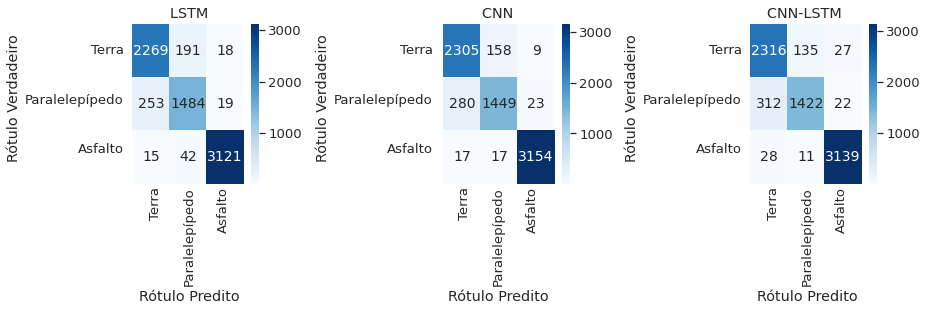
\includegraphics[width=1\textwidth]{figuras/fig_35.png}
  \fonte{Desenvolvido pelo autor.}
\end{figure}

\begin{table}[H]
\scriptsize
\centering
\caption{Métricas de avaliação para cada melhor modelo baseado em técnicas de \textit{deep learning}.} 
\label{table:deep_ml_metrics_tipo_superficie_1}
\begin{tabular}{clccc}
\toprule
\textbf{Modelo} & \multicolumn{1}{c}{\textbf{Classe de Dados}} & \textbf{F1-Score} & \textbf{Precisão} & \textbf{Recall} \\ \midrule
\multirow{4}{*}{LSTM} & Asfalto & 98.52\% & 98.83\% & 98.21\% \\ \cmidrule(l){2-5} 
 & Paralelepípedo & 85.46\% & 86.43\% & 84.51\% \\ \cmidrule(l){2-5} 
 & Terra & 90.49\% & 89.44\% & 91.57\% \\ \midrule
\multirow{4}{*}{CNN} & Asfalto & 98.96\% & 99.00\% & 98.93\% \\ \cmidrule(l){2-5} 
 & Paralelepípedo & 85.84\% & 89.23\% & 82.71\% \\ \cmidrule(l){2-5} 
 & Terra & 90.85\% & 88.59\% & 93.24\% \\ \midrule
\multirow{4}{*}{CNN-LSTM} & Asfalto & 98.62\% & 98.46\% & 98.77\% \\ \cmidrule(l){2-5} 
 & Paralelepípedo & 85.56\% & 90.69\% & 80.98\% \\ \cmidrule(l){2-5} 
 & Terra & 90.22\% & 87.20\% & 93.46\% \\ \bottomrule
\end{tabular}
\fonte{Desenvolvido pelo autor.}
\end{table}

Com base na \autoref{table:deep_ml_results_tipo_superficie_1}, é possível observar que as diferentes abordagens de \textit{Deep Learning} se mostraram adequadas para o problema de classificação proposto. Avaliando a média de acurácia em validação, o modelo baseado em CNN foi ligeiramente melhor do que os outros, embora o baseado em LSTM foi o melhor no experimento 3, o baseado em CNN melhor no experimento 1, e o baseado em CNN-LSTM melhor no experimento 2. Analisando a matriz de confusão na \autoref{fig:confusion_matrix_deep_tipo_superficie_1} e outras métricas de avaliação detalhadas na \autoref{table:deep_ml_metrics_tipo_superficie_1}, observamos que o modelo baseado em CNN tem os maiores valores de f1-score para todas as classes de dados, sendo o melhor modelo quando se considera não apenas sua capacidade de obter VP e VN, mas também de evitar FP e FN. Portanto, consideramos o modelo de CNN como o melhor modelo baseado em \textit{Deep Learning} para a classificação do tipo de superfície de pista devido a sua maior acurácia e valores de f1-score, além de ser o modelo com menor custo computacional entre os três modelos DNN. Sendo assim, a técnica obteve um valor de acurácia na validação de 93.17\%, classificando estrada de terra com valor f1-score de 90.85\%, paralelepípedo com 85.84\% e asfalto com 98.9\%, obtendo resultados melhores que os métodos clássicos e que os estudos relacionados, aplicando ainda variações contextuais.

\chapter{Classificação de Tipo de Superfície de Pista 2}
\label{cap:classificacao_tipo_superficie_2}

Através dos resultados obtidos no estudo da seção anterior, foi conduzido um segundo estudo para o desenvolvimento de modelo adaptativo de classificação de tipo de superfície de pista, com foco em modelos de \textit{Deep Learning}, os quais se mostraram mais promissores quando comparados a modelos de Aprendizado de Máquina clássicos. Neste estudo foi produzido em conjunto uma avaliação multiaspecto e multicontextual. O processo de desenvolvimento e experimentação é detalhado nas próximas subseções. Na primeira delas, o pré-processamento, os dados foram ajustados e organizados para avaliar aspectos como a influência do ponto de coleta de dados no veículo, o domínio de análise, as características de entrada do modelo e o tamanho da janela de dados. Também foi avaliada a capacidade de generalização do aprendizado dos modelos para contextos desconhecidos. Na segunda subseção, processamento, foram desenvolvidos três modelos de DNN baseados em diferentes técnicas de \textit{Deep Learning}: LSTM, GRU e CNN. Por fim, na última subseção são detalhados e comparados os resultados obtidos.

\section{Pré-Processamento}

Na etapa de pré-processamento os dados foram organizados e transformados para serem utilizados como entrada dos modelos de classificação. Esta etapa incluiu a separação de dados para treinamento e validação do modelo, a definição das características de entrada, a normalização dos dados das características e o agrupamento de dados em janelas. Neste estudo, foram utilizados os dados de aceleração em três eixos (X, Y, Z) e em três pontos de coleta diferentes (abaixo e próximo da suspensão, acima e próximo da suspensão e no painel de controle), juntamente com a taxa de rotação em três eixos e nos três pontos de coleta, além da velocidade do veículo.

Com o objetivo de avaliar a influência da propriedade de dependência veicular e verificar a viabilidade de um modelo de classificação para os dados coletados em diferentes locais do veículo, definimos os seguintes \emph{experimentos por colocação}, com base nos pontos de coleta de dados no veículo:

\begin{description}
	
	\item[Experimento por Colocação 1:] Foram utilizados os dados de força de aceleração 3D e taxa de rotação 3D amostrados próximo e abaixo da suspensão, mais a velocidade.
    
    \item[Experimento por Colocação 2:] Foram utilizados os dados de força de aceleração 3D e taxa de rotação 3D amostrados próximo e acima da suspensão, mais a velocidade.
    
    \item[Experimento por Colocação 3:] Foram utilizados os dados de força de aceleração 3D e taxa de rotação 3D amostrados no painel de controle, mais a velocidade.
    
\end{description}

Neste estudo, buscou-se identificar também o domínio de análise mais adequado para classificar o tipo de superfície de pista. Sendo assim, para cada \emph{experimento de colocação}, foram definidos \emph{experimentos por domínio de análise}. Para a análise no domínio da frequência, foram aplicados nos dados a Transformada de Fourier de Curto Tempo (\textit{Short-Time Fourier Transform} - STFT) para extrair as características de magnitude da frequência através de uma janela deslizante de 100 amostras com total sobreposição. Os \emph{experimentos por domínio de análise} foram definidos de acordo com as características de entrada detalhadas abaixo:

\begin{description}

    \item[Experimento por Domínio de Análise 1:] Foram utilizadas as 7 características correspondentes a aceleração nos eixos X, Y, Z; a taxa de rotação nos eixos X, Y, Z; e a velocidade.
    
    \item[Experimento por Domínio de Análise 2:] Foram utilizadas as 7 características do \emph{Experimento por Domínio de Análise 1}, mais quatro características de aceleração composta XY, YZ, XZ, XYZ, de acordo com as fórmulas detalhadas em \cite{Tan2019}.
    
    \item[Experimento por Domínio de Análise 3:] Foram utilizadas 357 características correspondentes às magnitudes das 51 frequências de cada uma das 7 características definidas no domínio do tempo em \emph{Experimento por Domínio de Análise 1}.
    
    \item[Experimento por Domínio de Análise 4:] Foram utilizadas 561 características correspondentes às magnitudes das 51 frequências de cada uma das 11 características definidas no domínio do tempo em \emph{Experimento por Domínio de Análise 2}.
    
\end{description}

Após definir os \emph{experimentos por domínio de análise}, os dados foram normalizados usando \textit{Min Max Scaler}. Os dados das características no domínio do tempo foram normalizados na faixa de [-1,1], uma vez que o sinal, neste caso, contém informações importantes, denotando a direção do vetor força. No domínio da frequência, como a magnitude não apresenta valores negativos, os dados foram normalizados na faixa de [0,1]. Em seguida, foram definidos os dados a serem usados no treinamento e na validação dos modelos. Para avaliar corretamente a generalização do aprendizado de cada técnica, avaliando sua adaptabilidade para contextos desconhecidos onde há variação nas propriedades de dependência veicular, de condução e ambiental, os dados de treinamento e validação foram divididos da mesma maneira que no estudo da seção anterior, separando-os de acordo com o conjunto de dados em três \emph{experimentos por contexto}:

\begin{description}
	
	\item[Experimento por Contexto 1:] O modelo aprende dados de todos os veículos e motoristas para alguns cenários; mas não todos os veículos com todos os motoristas para todos os cenários.
    \begin{itemize}
        \item \textbf{Treinamento (65\%):} PVS 1, PVS 3, PVS 4, PVS 6, PVS 7, PVS 9. 
        \item \textbf{Validação (35\%):} PVS 2, PVS 5, PVS 8.
    \end{itemize}
    
    \item[Experimento por Contexto 2:] O modelo aprende dados de todos os cenários para alguns veículos e alguns motoristas; mas não todos os veículos com todos os motoristas para todos os cenários.
    \begin{itemize}
        \item \textbf{Treinamento (66\%):} PVS 1, PVS 2, PVS 3, PVS 7, PVS 8, PVS 9.
        \item \textbf{Validação (34\%):} PVS 4, PVS 5, PVS 6.
    \end{itemize}
    
    \item[Experimento por Contexto 3:] O modelo aprende dados de alguns veículos com alguns motoristas para alguns cenários; mas não todos os veículos com todos os motoristas para todos os cenários.
    \begin{itemize}
        \item \textbf{Treinamento (66\%):} PVS 1, PVS 2, PVS 4, PVS 6, PVS 8, PVS 9.
        \item \textbf{Validação (34\%):} PVS 3, PVS 5, PVS 7.
    \end{itemize}
    
\end{description}

Finalmente, para analisar a influência do número de amostras na classificação, foram criados três \emph{experimentos por tamanho de janela de dados}, com janelas de 100, 200 e 300 amostras. A janela de dados utilizada foi fixa sem sobreposição, e cada amostra correspondeu a um vetor com os valores das características. Em resumo, cada experimento realizado neste estudo é um elemento do produto cartesiano entre \emph{experimentos por colocação}, \emph{experimentos por domínio de análise}, \emph{experimentos por contexto} e \emph{experimentos por tamanho de janela de dados}.

\section{Processamento}

Após a etapa de pré-processamento, os dados foram aplicados em modelos de classificação baseados em \textit{Deep Learning}. Neste estudo, foram desenvolvidas DNN baseadas em LSTM, GRU e CNN. Todos os modelos são sequenciais e utilizam o otimizador Adam em conjunto com a função de perda de Entropia Cruzada Categórica. O modelo baseado em LSTM é ilustrado na \autoref{fig:best_lstm_tipo_superficie_2}, sendo composto por um bloco de camada de entrada, três blocos de camadas de recorrência e regularização e um bloco de camadas totalmente conectadas para produção de saída. O bloco de entrada possui uma camada que recebe um tensor \emph{janelas x sequências x características}, onde \emph{janelas} são os agrupamentos de janelas, \emph{sequências} são os dados que compõem uma das janelas e \emph{características} os valores das 7 variáveis. Cada bloco de recorrência e regularização é composto por uma camada LSTM unidirecional de 100 unidades, seguido por uma camada de \textit{Batch Normalization} e outra de \textit{Dropout} em 50\%. Após o processamento nas camadas recorrentes, os parâmetros passam para o bloco de camadas totalmente conectadas, onde existem duas camadas \textit{Dense}, a primeira com 100 neurônios com ativação \textit{Relu} e a segunda com 3 neurônios e ativação \textit{Softmax}, produzindo a classificação. A saída esperada da rede são os rótulos correspondentes à última amostra na janela. O modelo baseado em GRU desenvolvido possuí a mesma estrutura LSTM, trocando camadas LSTM por GRU conforme detalha a \autoref{fig:best_gru_tipo_superficie_2}.

\begin{figure}[h!]
  \centering
  \caption{Modelo LSTM para classificação do tipo de superfície de pista}
  \label{fig:best_lstm_tipo_superficie_2}
  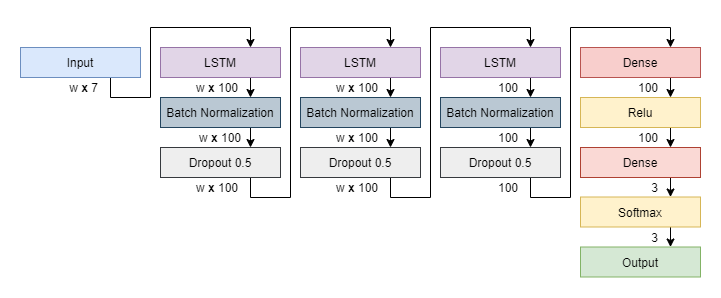
\includegraphics[width=0.8\textwidth]{figuras/fig_37.png}
 \fonte{Desenvolvido pelo autor.}
\end{figure}

\begin{figure}[h!]
  \centering
  \caption{Modelo GRU para classificação do tipo de superfície de pista}
  \label{fig:best_gru_tipo_superficie_2}
  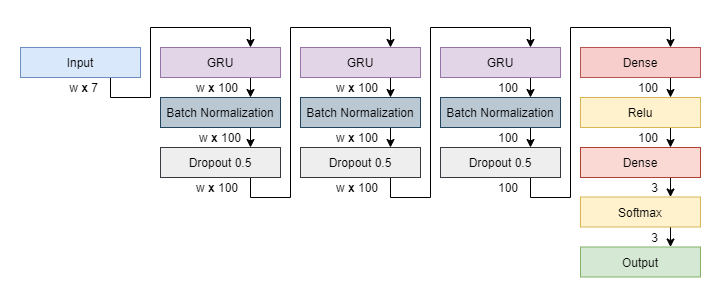
\includegraphics[width=0.8\textwidth]{figuras/fig_38.png}
 \fonte{Desenvolvido pelo autor.}
\end{figure}

\begin{figure}[h!]
  \centering
  \caption{Modelo CNN para classificação do tipo de superfície de pista}
  \label{fig:best_cnn_tipo_superficie_2}
  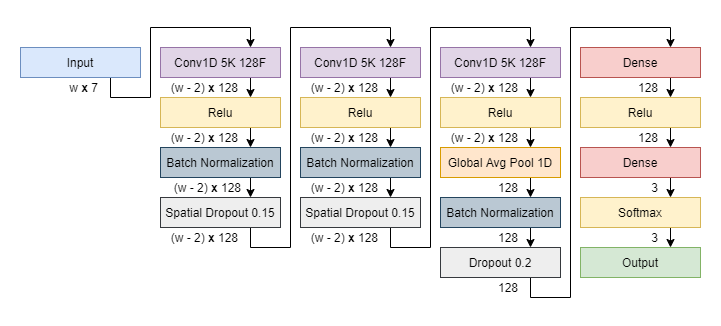
\includegraphics[width=0.8\textwidth]{figuras/fig_39.png}
 \fonte{Desenvolvido pelo autor.}
\end{figure}

Por fim, o modelo desenvolvido baseado em CNN é ilustrado na \autoref{fig:best_cnn_tipo_superficie_2}, sendo composto por um bloco de camada de entrada, três blocos de camadas de convolução e regularização e um bloco de camadas totalmente conectadas para produção de saída. O bloco de entrada possui uma camada que recebe um tensor \emph{janelas x sequências x características}, similar aos modelos LSTM e GRU. Os dois primeiros blocos de convolução e regularização são compostos cada um por uma camada Conv 1D com 128 filtros de \textit{kernel} tamanho 5 para extração de características e ativação \textit{Relu}, seguida por regularização através de uma camada de \textit{Batch Normalization} e outra de \textit{Spatial Dropout 1D} em 15\%. O último bloco de convolução e regularização possui uma camada Conv 1D com as mesmas configurações das anteriores, uma camada de \textit{Global Average Pooling 1D}, e camadas de regularização por \textit{Batch Normalization} e \textit{Dropout} em 20\%. Finalmente, o bloco de totalmente conectadas consiste em duas camadas \textit{Dense}, uma com 32 neurônios e ativação \textit{Relu} e outra com 3 neurônios e ativação \textit{Softmax}. A saída esperada da rede são os rótulos mais presentes na janela de dados.

\section{Análise de Resultados}

Todos os modelos desenvolvidos neste estudo foram programados em Python 3, utilizando a biblioteca Keras do Tensorflow. Os experimentos foram realizados no Google \textit{Collaboratory}, em um ambiente com as mesmas configurações do estudo da seção anterior. Todos os experimentos foram executados três vezes, %a fim de minimizar a aleatoriedade dos parâmetros iniciais,
recuperando apenas o melhor modelo entre as três execuções. O melhor modelo foi considerado aquele que apresentou o maior valor de acurácia durante a validação. Os resultados obtidos foram agrupados por ponto de coleta de dados no veículo, detalhados nas Tabelas \ref{table:below_suspension_results_tipo_superficie_2}, \ref{table:above_suspension_results_tipo_superficie_2} e \ref{table:dashboard_results_tipo_superficie_2}. Além do agrupamento por ponto de coleta, em cada tabela é detalhado o experimento por modelo de DNN, domínio de análise, características de entrada e janelas de dados. Cada valor exibido corresponde a média de acurácia na validação dos três \emph{experimentos por contexto}, os quais visam analisar a capacidade de aprendizado e generalização do modelo para cenários não conhecidos, onde há variações contextuais correspondentes aos fatores de dependência veicular, de condução e ambientais. Os valores destacados correspondem ao valor máximo de média de acurácia em validação para dado tipo de DNN.

\begin{table}[h!]
\scriptsize
\centering
\caption{Média de acurácia para colocação próximo e abaixo da suspensão}
\label{table:below_suspension_results_tipo_superficie_2}
\begin{tabular}{cccccc}
\cmidrule(l){4-6} & \multicolumn{1}{l}{\textbf{}} & \multicolumn{1}{l}{} & \multicolumn{3}{c}{\textbf{Tamanho da Janela de Dados}} \\ \midrule
\textbf{Modelo} & \textbf{Domínio} & \textbf{Características} & \multicolumn{1}{c}{100} & \multicolumn{1}{c}{200} & \multicolumn{1}{c}{300} \\ \midrule
\multirow{5}{*}{LSTM} & \multirow{2}{*}{Tempo} 
& 7 & 89,69\% & 92,06\% & 92,34\% \\ \cmidrule(l){3-6} 
&  & 11 & 89,70\% & 90,99\% & 92,11\% \\ \cmidrule(l){2-6} 
& \multirow{2}{*}{Frequência} 
& 357 & 90,34\% & 91,86\% & 92,63\% \\ \cmidrule(l){3-6} 
&  & 561 & 90,65\% & 91,55\% & \cellcolor[HTML]{34FF34}92,82\% \\ \midrule
\multirow{5}{*}{GRU} & \multirow{2}{*}{Tempo} 
& 7 & 90,23\% & 92,06\% & \cellcolor[HTML]{34FF34}92,88\% \\ \cmidrule(l){3-6} 
&  & 11 & 89,81\% & 91,65\% & 92,31\% \\ \cmidrule(l){2-6} 
 & \multirow{2}{*}{Frequência} & 357 & 90,18\% & 91,09\% & 92,33\% \\ \cmidrule(l){3-6} 
 &  & 561 & 90,55\% & 91,59\% & 92,40\% \\ \midrule
\multirow{5}{*}{CNN} & \multirow{2}{*}{Tempo} & 7 & 91,16\% & 92,92\% & 93,04\% \\ \cmidrule(l){3-6} 
 &  & 11 & 90,24\% & 92,58\% & 92,60\% \\ \cmidrule(l){2-6} 
 & \multirow{2}{*}{Frequência} & 357 & 89,56\% & 91,92\% & \cellcolor[HTML]{34FF34}93,91\% \\ \cmidrule(l){3-6} 
 &  & 561 & 89,78\% & 92,08\% & 93,67\% \\ \bottomrule
\end{tabular}
\fonte{Desenvolvido pelo autor.}
\end{table}

\begin{table}[h!]
\scriptsize
\centering
\caption{Média de acurácia para colocação próximo e acima da suspensão}
\label{table:above_suspension_results_tipo_superficie_2}
\begin{tabular}{cccccc}
\cmidrule(l){4-6}
 & \multicolumn{1}{l}{\textbf{}} & \multicolumn{1}{l}{} & \multicolumn{3}{c}{\textbf{Tamanho da Janela de Dados}} \\ \midrule
\textbf{Modelo} & \textbf{Domínio} & \textbf{Características} & \multicolumn{1}{c}{100} & \multicolumn{1}{c}{200} & \multicolumn{1}{c}{300} \\ \midrule
\multirow{5}{*}{LSTM} & \multirow{2}{*}{Tempo} & 7 & 89,23\% & 90,56\% & \cellcolor[HTML]{34FF34}90,89\% \\ \cmidrule(l){3-6} 
 &  & 11 & 87,56\% & 88,96\% & 90,58\% \\ \cmidrule(l){2-6} 
 & \multirow{2}{*}{Frequência} & 357 & 88,41\% & 89,55\% & 90,78\% \\ \cmidrule(l){3-6} 
 &  & 561 & 88,04\% & 90,00\% & 90,15\% \\ \midrule
\multirow{5}{*}{GRU} & \multirow{2}{*}{Tempo} & 7 & 87,53\% & 89,16\% & 89,42\% \\ \cmidrule(l){3-6} 
 &  & 11 & 87,54\% & 88,61\% & 89,79\% \\ \cmidrule(l){2-6} 
 & \multirow{2}{*}{Frequência} & 357 & 88,57\% & 89,49\% & \cellcolor[HTML]{34FF34}90,41\% \\ \cmidrule(l){3-6} 
 &  & 561 & 87,84\% & 89,76\% & 90,05\% \\ \midrule
\multirow{5}{*}{CNN} & \multirow{2}{*}{Tempo} & 7 & 88,65\% & 90,85\% & \cellcolor[HTML]{34FF34}92,02\% \\ \cmidrule(l){3-6} 
 &  & 11 & 88,25\% & 90,04\% & 90,74\% \\ \cmidrule(l){2-6} 
 & \multirow{2}{*}{Frequência} & 357 & 88,32\% & 90,75\% & 91,01\% \\ \cmidrule(l){3-6} 
 &  & 561 & 88,23\% & 90,67\% & 90,92\% \\ \bottomrule
\end{tabular}
\fonte{Desenvolvido pelo autor.}
\end{table}

\begin{table}[h!]
\scriptsize
\centering
\caption{Média de acurácia para colocação no painel de controle}
\label{table:dashboard_results_tipo_superficie_2}
\begin{tabular}{cccccc}
\cmidrule(l){4-6}
 & \multicolumn{1}{l}{\textbf{}} & \multicolumn{1}{l}{} & \multicolumn{3}{c}{\textbf{Tamanho da Janela de Dados}} \\ \midrule
\textbf{Modelo} & \textbf{Domínio} & \textbf{Características} & 100 & 200 & \multicolumn{1}{c}{300} \\ \midrule
\multirow{5}{*}{LSTM} & \multirow{2}{*}{Tempo} & 7 & 89,64\% & \cellcolor[HTML]{34FF34}91,79\% & 91,64\% \\ \cmidrule(l){3-6} 
 &  & 11 & 88,54\% & 90,96\% & 91,73\% \\ \cmidrule(l){2-6} 
 & \multirow{2}{*}{Frequência} & 357 & 88,61\% & 89,47\% & 90,92\% \\ \cmidrule(l){3-6} 
 &  & 561 & 89,90\% & 91,03\% & 91,55\% \\ \midrule
\multirow{5}{*}{GRU} & \multirow{2}{*}{Tempo} & 7 & 89,82\% & 91,67\% & \cellcolor[HTML]{34FF34}91,91\% \\ \cmidrule(l){3-6} 
 &  & 11 & 89,62\% & 90,83\% & 91,73\% \\ \cmidrule(l){2-6} 
 & \multirow{2}{*}{Frequência} & 357 & 88,76\% & 90,53\% & 90,74\% \\ \cmidrule(l){3-6} 
 &  & 561 & 89,67\% & 90,92\% & 91,68\% \\ \midrule
\multirow{5}{*}{CNN} & \multirow{2}{*}{Tempo} & 7 & 89,44\% & 91,46\% & 93,05\% \\ \cmidrule(l){3-6} 
 &  & 11 & 89,64\% & 91,50\% & 93,30\% \\ \cmidrule(l){2-6} 
 & \multirow{2}{*}{Frequência} & 357 & 89,40\% & 91,51\% & 92,37\% \\ \cmidrule(l){3-6} 
 &  & 561 & 89,70\% & 92,09\% & \cellcolor[HTML]{34FF34}93,57\% \\ \bottomrule
\end{tabular}
\fonte{Desenvolvido pelo autor.}
\end{table}


Através das tabelas de resultados, é possível observar que o tamanho da janela de dados pouco influencia o resultado final. Considerando todos os experimentos realizados, o aumento da janela de dados de 100 para 200 amostras aumentou em média cerca de 1,8\% a média de acurácia em validação, enquanto que o aumento de 200 amostras para 300 acrescentou cerca de 0,8\%. Em relação a utilização das variáveis brutas dos sensores (7 características) e a magnitude de suas frequências (357 características) quando comparadas a adição das variáveis de aceleração composta (11 características) e a magnitude das frequências (561 características) foi observado uma variação média de 0,1\% no valor de acurácia, sendo que em 54\% dos melhores experimentos não utilizaram da aceleração composta, e outros 46\% utilizaram. De maneira geral, a adição destas variáveis não se justifica, aumentando o custo computacional sem ter um aumento consistente de acurácia.

Em relação aos domínios de análise, tanto o domínio do tempo quanto o domínio da frequência obtiveram bons resultados. Quando comparados os experimentos com as variáveis no domínio do tempo com sua respectiva representação no domínio da frequência, metade dos experimentos foi melhor no domínio do tempo e a outra metade teve melhor desempenho no domínio da frequência. Contudo, a variação média de acurácia entre os domínios de análise é de apenas 0,05\% e, considerando o custo de transformação entre domínios e o aumento expressivo de características de entrada quando representadas no domínio da frequência, passando de 7 no domínio do tempo para 357 com sua representação na frequência, e de 11 no domínio do tempo para 561 com sua representação na frequência, o domínio do tempo mostra-se mais adequado.

Analisando os modelos de DNN propostos, observamos que todos obtiveram bons resultados, com pouca variação de resultados. Considerando todos os experimentos, a rede baseada em CNN obteve melhores resultados, seguida pela LSTM e pela GRU. Contudo, a variação média dos valores de acurácia entre os três modelos é menor que 1\%. Em relação aos diferentes pontos de coleta no veículo, observamos que as redes são capazes de classificar corretamente mesmo com interferência da dependência veicular. Em uma análise ampla, as redes têm mais facilidade em reconhecer os padrões dos dados amostrados próximo abaixo da suspensão, seguidos pelos amostrados no painel de controle e por fim os amostrados próximo e acima da suspensão. Contudo, a variação média de acurácia entre os pontos de coleta é pequena, cerca de 2\%.

Em uma análise macro de todos os experimentos, observamos que as redes propostas nas suas diversas variações de configuração de dados de entrada realizam a classificação de superfície de pista com bons valores de acurácia em validação, validando a hipótese deste estudo e evidenciando a capacidade das redes de \textit{Deep Learning} aprenderem as relações dos dados com as propriedades de dependência, generalizando para cenários desconhecidos. Com base em todas as análises individuais realizadas, consideramos o melhor modelo de classificação de pista o modelo baseado em CNN, processando no domínio do tempo 7 características correspondentes aos dados brutos dos sensores, em uma janela de dados de 300 amostras. A Tabela \ref{table:cnn_results_tipo_superficie_2} detalha os valores de acurácia em treinamento e validação do modelo CNN para cada \emph{experimento por contexto} e \emph{experimento por colocação}. A \autoref{table:cnn_metrics_tipo_superficie_2} detalha as demais métricas de avaliação e a \autoref{fig:cnn_confusion_matrix_tipo_superficie_2} detalha as matrizes de confusão correspondentes.

\begin{table}[h!]
\scriptsize
\centering
\caption{Valores de acurácia para o modelo baseado em CNN}
\label{table:cnn_results_tipo_superficie_2}
\begin{tabular}{cccccc}
\toprule
\multirow{2}{*}{\textbf{\begin{tabular}[c]{@{}c@{}}Experimento \\ por Colocação\end{tabular}}} & \multirow{2}{*}{\textbf{\begin{tabular}[c]{@{}c@{}}Fase de \\ Processamento\end{tabular}}} & \multicolumn{4}{c}{\textbf{Experimento por Contexto}} \\ \cmidrule(l){3-6} 
 &  & 1 & 2 & 3 & Média \\ \midrule
\multirow{2}{*}{\begin{tabular}[c]{@{}c@{}}Próximo e abaixo \\ da suspensão\end{tabular}} & Treinamento & 94,67\% & 94,40\% & 97,01\% & 95,36\% \\ \cmidrule(l){2-6} 
 & Validação & 94,78\% & 92,17\% & 92,17\% & 93,04\% \\ \midrule
\multirow{2}{*}{\begin{tabular}[c]{@{}c@{}}Próximo e acima\\ da suspensão\end{tabular}} & Treinamento & 88,46\% & 92,89\% & 95,45\% & 92,27\% \\ \cmidrule(l){2-6} 
 & Validação & 94,11\% & 90,14\% & 91,80\% & 92,02\% \\ \midrule
\multirow{2}{*}{Painel de Controle} & Treinamento & 93,16\% & 94,84\% & 97,50\% & 95,17\% \\ \cmidrule(l){2-6} 
 & Validação & 95,25\% & 89,93\% & 93,96\% & 93,05\% \\ \bottomrule
\end{tabular}
\fonte{Desenvolvido pelo autor.}
\end{table}

\begin{table}[h!]
\scriptsize
\centering
\caption{Métricas de avaliação para o modelo baseado em CNN}
\label{table:cnn_metrics_tipo_superficie_2}
\begin{tabular}{clccc}
\toprule
\textbf{Colocação} & \multicolumn{1}{c}{\textbf{Classe de Dados}} & \textbf{F1-Score} & \textbf{Precisão} & \textbf{Recall} \\ \midrule
\multirow{4}{*}{\begin{tabular}[c]{@{}c@{}}Próximo e abaixo\\ da suspensão\end{tabular}} & Asfalto & 98,60\% & 98,59\% & 98,62\% \\ \cmidrule(l){2-5} 
 & Paralelepípedo & 86,09\% & 88,39\% & 83,90\% \\ \cmidrule(l){2-5} 
 & Terra & 90,78\% & 89,22\% & 92,39\% \\ \midrule
\multirow{4}{*}{\begin{tabular}[c]{@{}c@{}}Próximo e acima\\ da suspensão\end{tabular}} & Asfalto & 98,76\% & 99,08\% & 98,43\% \\ \cmidrule(l){2-5} 
 & Paralelepípedo & 84,18\% & 83,49\% & 84,87\% \\ \cmidrule(l){2-5} 
 & Terra & 89,06\% & 89,20\% & 88,91\% \\ \midrule
\multirow{4}{*}{Painel de Controle} & Asfalto & 98,62\% & 98,23\% & 99,02\% \\ \cmidrule(l){2-5} 
 & Paralelepípedo & 85,47\% & 90,13\% & 81,27\% \\ \cmidrule(l){2-5} 
 & Terra & 91,12\% & 88,58\% & 93,81\% \\ \bottomrule
\end{tabular}
\fonte{Desenvolvido pelo autor.}
\end{table}

\begin{figure}[h!]
  \centering
  \caption{Matriz de confusão para o modelo de CNN em cada ponto de coleta de dados}
  \label{fig:cnn_confusion_matrix_tipo_superficie_2}
  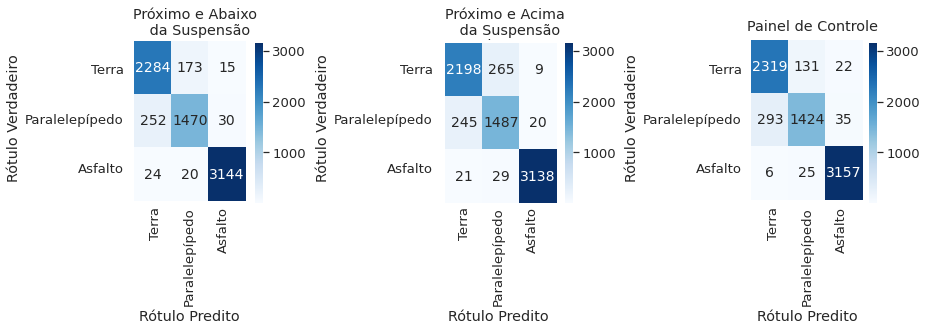
\includegraphics[width=1\textwidth]{figuras/fig_36.png}
  \fonte{Desenvolvido pelo autor.}
\end{figure}

Através das Tabelas \ref{table:cnn_results_tipo_superficie_2} e \ref{table:cnn_metrics_tipo_superficie_2}, e da \autoref{fig:cnn_confusion_matrix_tipo_superficie_2} observamos que a rede CNN demonstrou boa capacidade de aprendizado e generalização para todos os pontos de coleta e todas as variações de contexto. Para os dados amostrados próximo e abaixo da suspensão, a rede obteve média de acurácia de treinamento de 95,36\% e de 93,04\% em validação, classificando segmentos de asfalto com \textit{f1-score} de 98,60\%, paralelepípedo com 86,09\% e terra com 90,78\%. Para os dados amostrados próximo e acima da suspensão, o modelo obteve média de acurácia em treinamento de 92,27\% e de 92,02\% em validação, classificando segmentos de asfalto com \textit{f1-score} de 98,76\%, paralelepípedo com 84,18\% e terra com 86,06\%. Por fim, para os dados amostrados no painel de controle obteve-se média de acurácia em treinamento de 95,17\% e de 93,05\% em validação, classificando segmentos de asfalto com \textit{f1-score} de 98,62\%, paralelepípedo com 85,47\% e terra com 91,12\%. Observa-se que os resultados obtidos são superiores aos estudos anteriores, adicionando-se que neste estudo a análise foi realizada em contextos com variações das propriedades de dependência.
\chapter{Classificação de Qualidade de Superfície de Pista}
\label{cap:classificacao_qualidade}

Nesta seção é apresentado o estudo, desenvolvimento e experimentação voltado ao desenvolvimento de um modelo adaptativo para classificação da qualidade de superfície da pista. Baseado nos resultados dos experimentos das seções anteriores, este estudo focou no desenvolvimento de modelos baseados em \textit{Deep Learning}. O processo de desenvolvimento e experimentação é detalhado nas próximas subseções. Na primeira delas, de pré-processamento, foi realizada a seleção de variáveis, padronizados seus dados através de normalização dos sinais, e definidos experimentos para avaliar aspectos como ponto de coleta de dados no veículo, tamanho da janela de dados e variações contextuais, onde foi possível analisar a capacidade de generalização do aprendizado dos modelos para contextos desconhecidos e, portanto, avaliar sua adaptabilidade. Na segunda subseção, de processamento, foram desenvolvidos cinco modelos de DNN baseados em diferentes técnicas de \textit{Deep Learning}: LSTM, GRU, CNN, CNN-LSTM e ConvLSTM. Por fim, na última subseção são detalhados e comparados os resultados obtidos.

\section{Pré-Processamento}

Com base nos resultados obtidos nos experimentos anteriores, neste estudo utilizamos como características de entrada os dados brutos das variáveis de aceleração em três eixos (X, Y, Z) e em três diferentes pontos de coleta (abaixo e próximo da suspensão, acima e próximo da suspensão e painel de controle), juntamente com os dados de taxa rotação em três eixos e em três diferentes pontos de coleta, além da velocidade do veículo. Inicialmente, todos os dados foram normalizados com \textit{Robust Scaler}, o qual utilizando intervalo interquartil se mostra um escalador mais robusto para dados com \textit{outliers} \cite{Vaitheeshwari2019}. Os dados das características foram normalizados mantendo o sinal, uma vez que o sinal contém informação importante de direção do vetor de força. Após a normalização dos dados, para avaliar a influência da propriedade de dependência veicular e verificar a viabilidade de um modelo de classificação para os dados coletados em diferentes pontos do veículo, foram definidos os seguintes \emph{experimentos por colocação}, com base nos pontos de coleta de dados no veículo:

\begin{description}
	
	\item[Experimento por Colocação 1:] Foram utilizados os dados de força de aceleração 3D e taxa de rotação 3D amostrados próximo e abaixo da suspensão, mais a velocidade.
    
    \item[Experimento por Colocação 2:] Foram utilizados os dados de força de aceleração 3D e taxa de rotação 3D amostrados próximo e acima da suspensão, mais a velocidade.
    
    \item[Experimento por Colocação 3:] Foram utilizados os dados de força de aceleração 3D e taxa de rotação 3D amostrados no painel de controle, mais a velocidade.
    
\end{description}

Para avaliar a capacidade de generalização do aprendizado de cada técnica, avaliando sua adaptabilidade para contextos desconhecidos onde há variação nas propriedades de dependência veicular, de condução e ambiental, os dados de treinamento e validação foram divididos da mesma maneira que as pesquisas das seções anteriores, separando-os de acordo com o conjunto de dados em três \emph{experimentos por contexto}:

\begin{description}
	
	\item[Experimento por Contexto 1:] O modelo aprende dados de todos os veículos e motoristas para alguns cenários; mas não todos os veículos com todos os motoristas para todos os cenários.
    \begin{itemize}
        \item \textbf{Treinamento (65\%):} PVS 1, PVS 3, PVS 4, PVS 6, PVS 7, PVS 9. 
        \item \textbf{Validação (35\%):} PVS 2, PVS 5, PVS 8.
    \end{itemize}
    
    \item[Experimento por Contexto 2:] O modelo aprende dados de todos os cenários para alguns veículos e alguns motoristas; mas não todos os veículos com todos os motoristas para todos os cenários.
    \begin{itemize}
        \item \textbf{Treinamento (66\%):} PVS 1, PVS 2, PVS 3, PVS 7, PVS 8, PVS 9.
        \item \textbf{Validação (34\%):} PVS 4, PVS 5, PVS 6.
    \end{itemize}
    
    \item[Experimento por Contexto 3:] O modelo aprende dados de alguns veículos com alguns motoristas para alguns cenários; mas não todos os veículos com todos os motoristas para todos os cenários.
    \begin{itemize}
        \item \textbf{Treinamento (66\%):} PVS 1, PVS 2, PVS 4, PVS 6, PVS 8, PVS 9.
        \item \textbf{Validação (34\%):} PVS 3, PVS 5, PVS 7.
    \end{itemize}
    
\end{description}

Finalmente, para analisar a influência do número de amostras na classificação, foram criados três \emph{experimentos por tamanho de janela de dados}, com janelas de 100, 200, 300, 400, e 500 amostras. A janela de dados utilizada foi fixa sem sobreposição, e cada amostra correspondeu a um vetor com os valores das características. Em resumo, cada experimento realizado neste estudo é um elemento do produto cartesiano entre \emph{experimentos por colocação}, \emph{experimentos por contexto} e \emph{experimentos por tamanho de janela de dados}. Para avaliar a necessidade de aplicar técnicas de balanceamento de classe de dados, foi medida a distribuição de cada classe conforme detalhado na \autoref{table:distribuicao_classes_qualidade_superficie}. A distribuição de classes foi calculada com os dados de treinamento \cite{He2013,Kuhn2013}, uma vez que estes são os dados utilizados pelos modelos para aprender os padrões. A distribuição foi calculada em relação ao número de amostras, uma vez que as janelas de dados são definidas de acordo com esse parâmetro.

\begin{table}[h]
\caption{Distribuição de classes de dados de qualidade de superfície de pista}
\label{table:distribuicao_classes_qualidade_superficie}
\centering
\scriptsize
\begin{tabular}{lcccccc}
\cmidrule(l){2-7}
\multicolumn{1}{c}{\multirow{2}{*}{\textbf{}}} & 
\multicolumn{6}{c}{\textbf{Classe de Dados}} \\ \cmidrule(l){2-7} 
\multicolumn{1}{c}{} & 
\multicolumn{2}{c}{\textbf{Bom}} & 
\multicolumn{2}{c}{\textbf{Regular}} & 
\multicolumn{2}{c}{\textbf{Ruim}} \\ \midrule
\textbf{Fonte de Dados} & 
\textit{\textbf{Percentual}} & 
\textit{\textbf{Proporção}} & 
\textit{\textbf{Percentual}} & 
\textit{\textbf{Proporção}} & 
\textit{\textbf{Percentual}} & 
\textit{\textbf{Proporção}} \\ \midrule
Exp. por Contexto 1 & 41,69\% & 1:1,4 & 47,73\% & 1:1,1 & 10,58\% & 1:8,5 \\ \midrule
Exp. por Contexto 2 & 43,53\% & 1:1,3 & 40,17\% & 1:1,5 & 16,30\% & 1:5,1 \\ \midrule
Exp. por Contexto 3 & 42,51\% & 1:1,4 & 40,64\% & 1:1,5 & 16,85\% & 1:4,9 \\ \bottomrule
\end{tabular}
\fonte{Desenvolvido pelo autor.}
\end{table}

Analisando a \autoref{table:distribuicao_classes_qualidade_superficie}, observamos que a distribuição das classes de qualidade de superfície de pista situa-se entre 10,58\% e 47,73\%, dependendo do experimento. A proporção varia entre 1:1,1 a 1:8,5, onde para 1 amostra de uma determinada classe de dados, existem de 1,1 a 8,5 amostras nas outras classes. O desbalanceamento de classes pode ser considerado leve ou severo, onde as proporções de distribuição que variam de 1:4 até 1:100 (presença de 20\% - 1\%) são consideradas desbalanceamento leve e proporções de distribuição que variam de 1:100 ou mais (<1\% de presença) são consideradas desbalanceamentos severos \cite{Krawczyk2016,Brownlee2020}. Como podemos observar, as proporções de distribuição das classes de dados neste estudo em sua maioria não são classificadas sequer como desbalanceamento leve, e os poucos que são desbalanceamento leve, não há tendência a desbalanceamento severo. Sendo assim, este estudo não necessita de aplicação de técnica para balanceamento de classes. Com a definição dos experimentos, convêm ressaltar a diferença entre o modelo de GT de anotação automatizada por máquina e o modelo que se busca obter com estes experimentos. No primeiro, os três modelos de KMC gerados estão cada um deles em função de um dos veículos. Já neste estudo, os experimentos buscam por um único modelo que se adapte aos três veículos.

\section{Processamento}

Após o pré-processamento, os dados foram aplicados em cinco modelos de \textit{Deep Learning}, sendo baseados em LSTM, GRU, CNN, CNN-LSTM e ConvLSTM. Todos os modelos desenvolvidos são sequenciais e utilizam o otimizador Adam em conjunto com a função de perda Entropia Cruzada Categórica. Todos os modelos tiveram seus hiperparâmetros ajustados (\textit{hyperparameter tuning}) utilizando o algoritmo \textit{HyperBand} implementado na biblioteca Keras Tuner, onde foram testados diferentes tipos de camadas, número de camadas e neurônios, funções de ativação e várias outras características para encontrar o conjunto ideal de hiperparâmetros para cada DNN. 

O melhor modelo baseado em LSTM obtido através do ajuste de hiperparâmetros é detalhado na \autoref{fig:best_lstm_qualidade_superficie}. O modelo DNN é composto de um bloco de camada de entrada, três blocos de camadas de recorrência e regularização e três blocos de camada totalmente conectadas para produção da saída. O bloco de entrada possui uma camada que recebe um tensor \emph{janelas x sequências x características}, onde \emph{janelas} são os agrupamentos de todas as janelas de dados, \emph{sequências} são as sequências de dados para cada janela, e \emph{características} são os valores das variáveis de entrada. Cada bloco de recorrência e regularização é composto por uma camada LSTM unidirecional de 64 unidades, seguida por uma camada de \textit{Batch Normalization} e uma camada de \textit{Dropout} em 35\%. Após o processamento nas camadas recorrentes, os parâmetros são passados para os blocos totalmente conectados, onde existem duas camadas \textit{Dense} com 160 neurônios e ativação \textit{Sigmoid}, e uma camada \textit{Dense} com 3 neurônios e ativação \textit{Softmax}, produzindo a classificação. A saída esperada são os rótulos mais presentes na janela de dados.

\begin{figure}[h!]
  \centering
  \caption{Modelo LSTM para classificação de qualidade de superfície de pista}
  \label{fig:best_lstm_qualidade_superficie}
  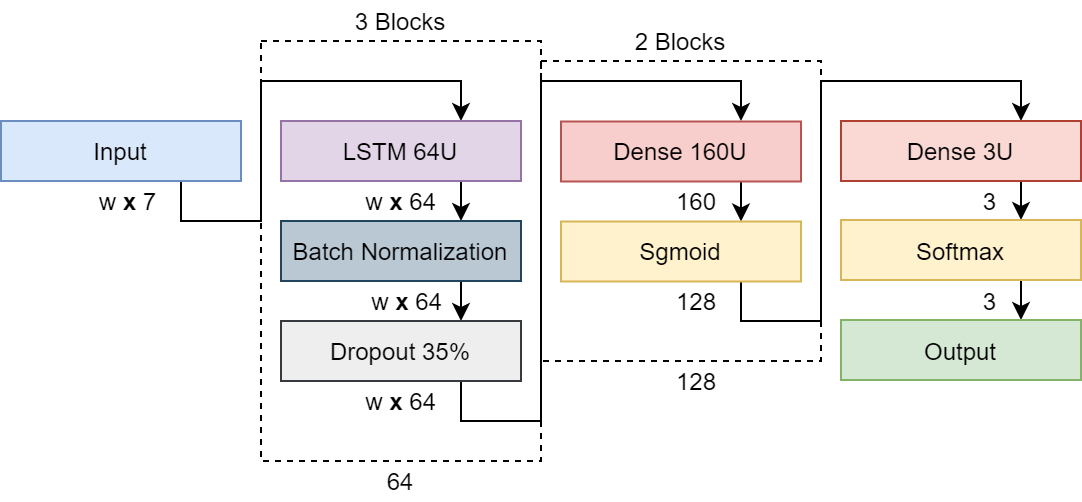
\includegraphics[width=0.7\textwidth]{figuras/fig_46.png}
 \fonte{Desenvolvido pelo autor.}
\end{figure}

O melhor modelo baseado em GRU obtido neste estudo é detalhado na \autoref{fig:best_gru_qualidade_superficie}. O modelo de DNN é composto de um bloco de camada de entrada, três blocos de camadas de recorrência e regularização e um bloco de camadas totalmente conectadas para produção de saída. O bloco de entrada possui uma camada que recebe um tensor \emph{janelas x sequências x características}, semelhante ao baseado em LSTM. Cada bloco de recorrência e regularização é composto por uma camada GRU unidirecional de 32 unidades, seguida por uma camada de \textit{Batch Normalization} e uma camada de \textit{Dropout} em 50\%. Após o processamento nas camadas recorrentes, os parâmetros passam para um bloco totalmente conectado, onde existe uma camada \textit{Dense} com 3 neurônios e ativação \textit{Softmax}, produzindo a classificação.

\begin{figure}[h!]
  \centering
  \caption{Modelo GRU para classificação de qualidade de superfície de pista}
  \label{fig:best_gru_qualidade_superficie}
  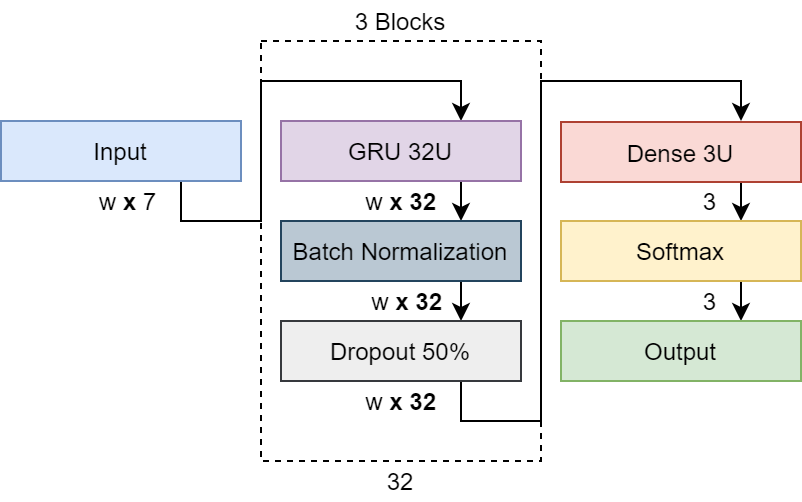
\includegraphics[width=0.5\textwidth]{figuras/fig_47.png}
 \fonte{Desenvolvido pelo autor.}
\end{figure}

O melhor modelo baseado em CNN obtido é detalhado na \autoref{fig:best_cnn_qualidade_superficie}. O modelo de DNN é composto de um bloco de entrada, dois blocos de convolução e regularização e um bloco de camadas totalmente conectadas para produção de saída. O bloco de entrada possui uma camada que recebe um tensor \emph{janelas x sequências x características}, semelhante aos modelos baseados em LSTM e GRU. O primeiro bloco de convolução e regularização é composto por uma camada Conv 1D com 224 filtros com \textit{kernel} de tamanho 7 para extração de características e ativação \textit{Relu}, seguida de regularização através de uma camada de \textit{Batch Normalization} e uma camada de \textit{Spatial Dropout 1D} em 50\%. O último bloco de convolução e regularização tem uma camada Conv 1D com as mesmas configurações do anterior, uma camada \textit{Global Max Pooling 1D} para extrair recursos mais robustos por meio dos valores máximos em cada região, e camadas de regularização por \textit{Batch Normalization 1D} e \textit{Dropout} em 40\%. Finalmente, o bloco totalmente conectado consiste de uma camada \textit{Dense} com 3 neurônios e ativação \textit{Softmax}, produzindo a classificação.

\begin{figure}[h!]
  \centering
  \caption{Modelo CNN para classificação de qualidade de superfície de pista}
  \label{fig:best_cnn_qualidade_superficie}
  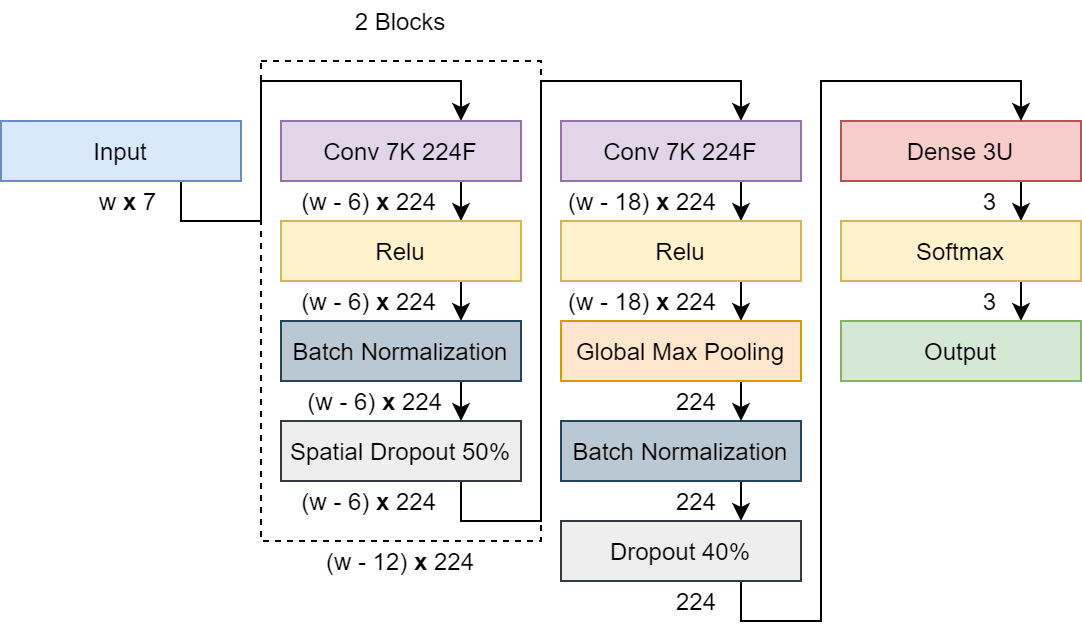
\includegraphics[width=0.7\textwidth]{figuras/fig_48.png}
 \fonte{Desenvolvido pelo autor.}
\end{figure}

O melhor modelo híbrido baseado em CNN-LSTM obtido é detalhado na \autoref{fig:best_cnn_lstm_qualidade_superficie}. O modelo de DNN é composto de um bloco de entrada, dois blocos de convolução e regularização, dois blocos recorrentes e de regularização e dois blocos de camada totalmente conectadas para produção de saída. O bloco de entrada tem uma camada que recebe um tensor \emph{janelas x sequências x subsequências x características}, onde \emph{janelas} são os agrupamentos de todas as janelas de dados, \emph{sequências} são as sequências de dados para cada janela, \emph{subsequências} são as subpartes da sequência de dados original, e \emph{características} os valores das variáveis de entrada. O primeiro bloco de convolução e regularização é composto por uma camada Conv 1D com 64 filtros com \textit{kernel} de tamanho 3 para extração de características e ativação \textit{Relu}, seguida de regularização através de uma camada de \textit{Batch Normalization} e uma camada de \textit{Spatial Dropout 1D} em 15\%. O último bloco de convolução e regularização tem uma camada Conv 1D com as mesmas configurações do anterior, uma camada \textit{Global Average Pooling 1D} para extrair recursos mais robustos por meio da média dos valores em cada região, uma camada \textit{Flatten} para reagrupar os recursos extraídos na sequência temporal original, e regularização por camada de \textit{Batch Normalization}. Em seguida, cada bloco de recorrência e regularização é composto por uma camada LSTM unidirecional de 64 unidades, seguida por uma camada de \textit{Batch Normalization} e uma camada de \textit{Dropout} em 45\%. Finalmente, os parâmetros resultantes passam para duas camadas \textit{Dense}, a primeira com 128 neurônios e ativação de \textit{Relu}, e a segunda com 3 neurônios e ativação de \textit{Softmax}, produzindo a classificação. 

\begin{figure}[h!]
  \centering
  \caption{Modelo CNN-LSTM para classificação de qualidade de superfície de pista}
  \label{fig:best_cnn_lstm_qualidade_superficie}
  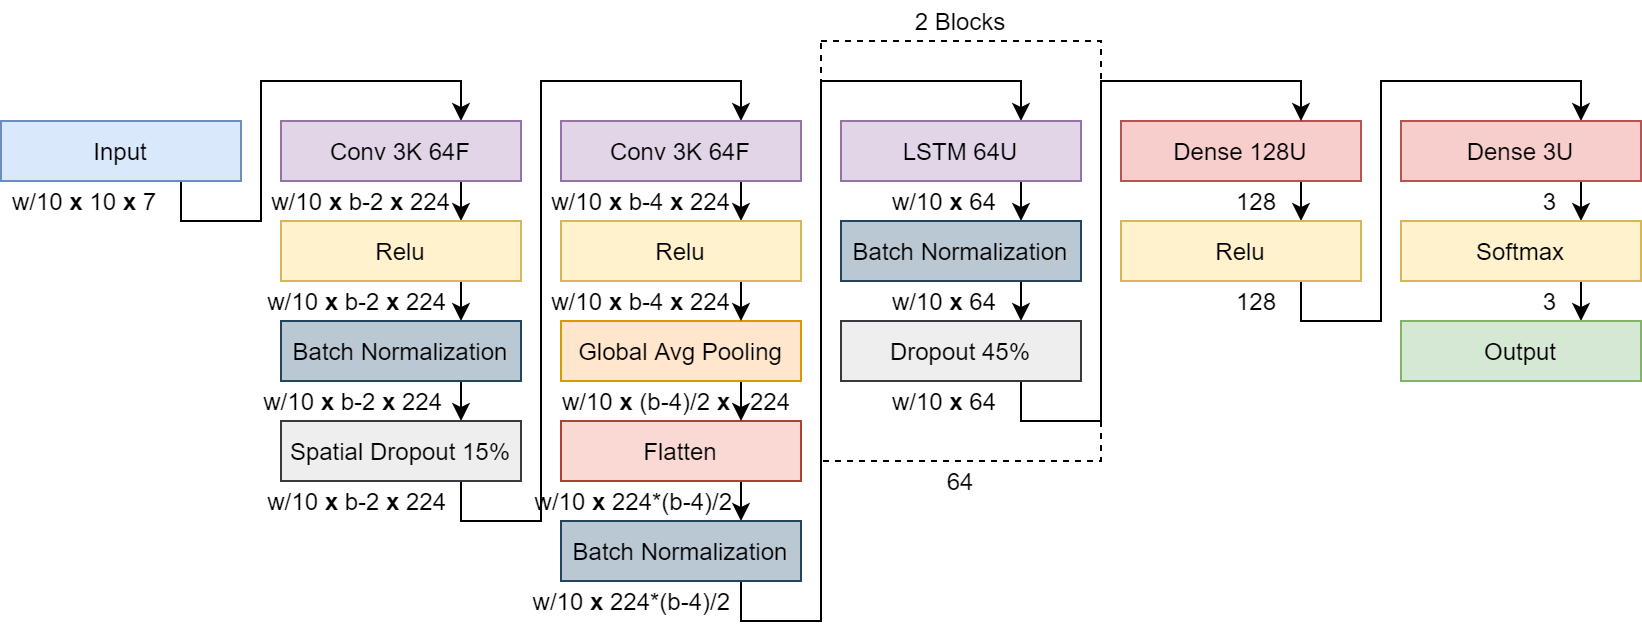
\includegraphics[width=1\textwidth]{figuras/fig_49.png}
 \fonte{Desenvolvido pelo autor.}
\end{figure}

O melhor modelo baseado em ConvLSTM obtido é detalhado na Figura \autoref{fig:best_conv_lstm_qualidade_superficie}. O modelo de DNN é composto de um bloco de entrada, um bloco convolucional recorrente e de regularização, e dois blocos de camadas totalmente conectadas para produção de saída. O bloco de entrada possui uma camada que recebe um tensor \emph{janelas x sequências x subsequências x características}, semelhante ao modelo CNN-LSTM. O bloco convolucional recorrente e de regularização é composto por uma camada \textit{ConvLSTM 1D} com 224 filtros \textit{kernel} de tamanho 7 e ativação \textit{Relu}, seguido por regularização através de uma camada \textit{Dropout} em 35\%. Finalmente, os parâmetros resultantes são achatados (\textit{flattened)} e passados para duas camadas \textit{Dense}, a primeira com 160 neurônios e ativação \textit{Relu}, e a segunda com 3 neurônios e ativação \textit{Softmax}, produzindo a classificação.

\begin{figure}[ht!]
  \centering
  \caption{Modelo ConvLSTM para classificação de qualidade de superfície de pista}
  \label{fig:best_conv_lstm_qualidade_superficie}
  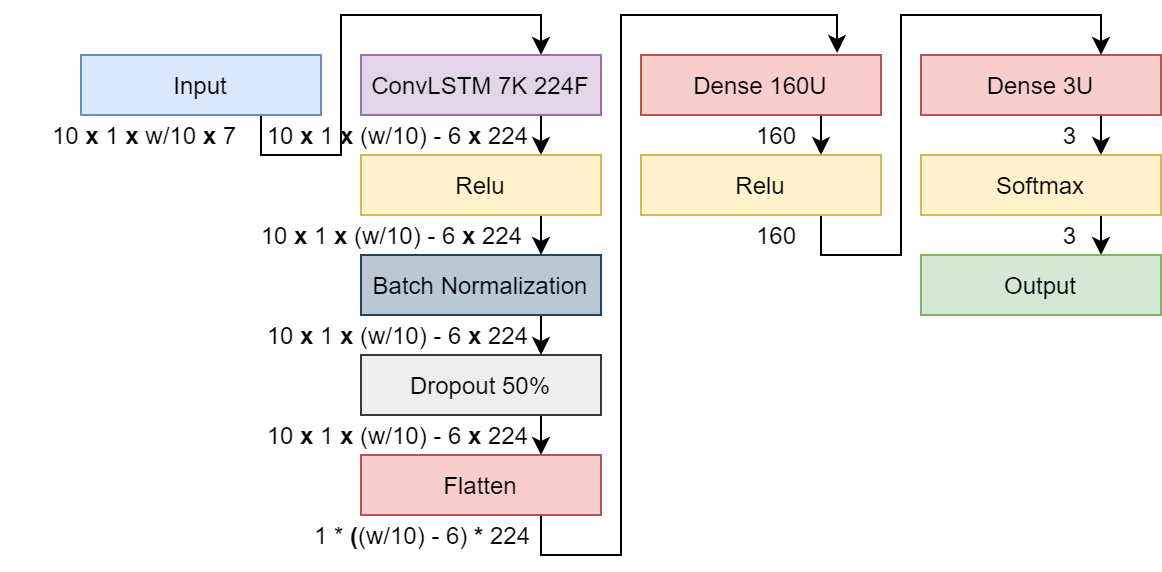
\includegraphics[width=0.7\textwidth]{figuras/fig_50.png}
 \fonte{Desenvolvido pelo autor.}
\end{figure}

\newpage
\section{Análise de Resultados}

Neste estudo todos os modelos de classificação de qualidade de superfície foram desenvolvidos na linguagem Python 3, utilizando da biblioteca Keras 2, a qual é uma API de alto nível do TensorFlow. Os hiperparâmetros dos modelos foram afinados através da biblioteca Keras Tuner. Todos os experimentos foram executados em máquinas do Google \textit{Collaboratory}, com as mesmas configurações dos estudos das seções anteriores. Cada experimento executado é um elemento do produto Cartesiano entre \emph{experimentos por colocação}, \emph{experimentos por contexto} e \emph{experimentos por tamanho da janela de dados}. Cada experimento foi executado três vezes, para minimizar a aleatoriedade de parâmetros iniciais, como pesos sinápticos, recuperando-se o melhor das três execuções. Consideramos a melhor execução aquele com maior valor de acurácia na fase de validação, uma vez que o treinamento dos modelos foi configurado para maximizar a métrica de acurácia.

Os resultados obtidos com a execução de todos os experimentos são apresentados nas Tabelas \ref{table:lstm_accuracy_result_qualidade_superficie} a \ref{table:conv_lstm_accuracy_result_qualidade_superficie}. Em cada tabela são detalhados os resultados para determinado modelo de DNN, para cada colocação, contexto e janela de dados. Também são apresentadas métricas de média aritmética para cada tipo de experimento, sendo Acurácia Média dos Experimentos por Contexto (AMEC) e Acurácia Média dos Experimentos por Contexto e Colocação (AMECC), onde são destacados os menores e maiores valores de acurácia obtidos na fase de validação.

\begin{table}[H]
\scriptsize
\centering
\caption{Valores de acurácia em validação obtidos pelo modelo LSTM} 
\label{table:lstm_accuracy_result_qualidade_superficie}
\begin{tabular}{ccccccc}
\toprule
\multicolumn{2}{c}{\textbf{Tipo de Experimento}} & \multicolumn{5}{c}{\textit{\textbf{Tamanho da Janela de Dados}}} \\ \midrule
\textit{\textbf{Colocação}} & \textit{\textbf{Contexto}} & \textit{100} & \textit{200} & \textit{300} & \textit{400} & \textit{500} \\ \midrule
\multirow{4}{*}{\begin{tabular}[c]{@{}c@{}} \\ Próximo e Abaixo \\ da Suspensão\end{tabular}} 
& 1 & 89,79\% & 90,89\% & 91,40\% & 91,67\% & 91,61\% \\ \cmidrule(l){2-7} 
& 2 & 90,37\% & 91,31\% & 93,00\% & 92,49\% & 90,94\% \\ \cmidrule(l){2-7} 
& 3 & 91,42\% & 92,20\% & 92,90\% & 92,00\% & 92,99\% \\ \cmidrule(l){2-7} 
& AMEC & \cellcolor[HTML]{FFCCC9}90,53\% & 91,47\% & \cellcolor[HTML]{34FF34}92,43\% & 92,05\% & 91,85\% \\ \midrule
\multirow{4}{*}{\begin{tabular}[c]{@{}c@{}} \\ Próximo e Acima \\ da Suspensão\end{tabular}} 
& 1 & 90,14\% & 91,10\% & 92,42\% & 92,03\% & 91,55\% \\ \cmidrule(l){2-7} 
& 2 & 90,63\% & 92,11\% & 92,34\% & 92,27\% & 91,42\% \\ \cmidrule(l){2-7} 
& 3 & 91,54\% & 92,26\% & 92,50\% & 93,04\% & 91,56\% \\ \cmidrule(l){2-7} 
& AMEC & \cellcolor[HTML]{FFCCC9}90,77\% & 91,82\% & 92,42\% & \cellcolor[HTML]{34FF34}92,44\% & 91,51\% \\ \midrule
\multirow{4}{*}{\begin{tabular}[c]{@{}c@{}} \\ Painel de Controle \end{tabular}} 
& 1 & 90,45\% & 90,60\% & 92,50\% & 89,83\% & 88,86\% \\ \cmidrule(l){2-7} 
& 2 & 87,96\% & 88,36\% & 91,55\% & 90,39\% & 90,11\% \\ \cmidrule(l){2-7} 
& 3 & 91,46\% & 91,68\% & 92,09\% & 92,71\% & 92,31\% \\ \cmidrule(l){2-7} 
& AMEC & \cellcolor[HTML]{FFCCC9}89,95\% & 90,21\% & \cellcolor[HTML]{34FF34}92,05\% & 90,98\% & 90,43\% \\ \midrule
& AMECC & \cellcolor[HTML]{FFCCC9}90,42\% & 91,17\% & \cellcolor[HTML]{34FF34}92,30\% & 91,82\% & 91,26\% \\ \cmidrule(l){2-7} 
\end{tabular}
\fonte{Desenvolvido pelo autor.}
\end{table}

\begin{table}[H]
\scriptsize
\centering
\caption{Valores de acurácia em validação obtidos pelo modelo GRU} 
\label{table:gru_accuracy_result_qualidade_superficie}
\begin{tabular}{ccccccc}
\toprule
\multicolumn{2}{c}{\textbf{Tipo de Experimento}} & \multicolumn{5}{c}{\textit{\textbf{Tamanho da Janela de Dados}}} \\ \midrule
\textit{\textbf{Colocação}} & \textit{\textbf{Contexto}} & \textit{100} & \textit{200} & \textit{300} & \textit{400} & \textit{500} \\ \midrule
\multirow{4}{*}{\begin{tabular}[c]{@{}c@{}} \\ Próximo e Abaixo \\ da Suspensão\end{tabular}} 
& 1 & 90,27\% & 91,20\% & 92,26\% & 91,61\% & 92,73\%  \\ \cmidrule{2-7}
& 2 & 90,89\% & 92,08\% & 92,75\% & 92,21\% & 91,98\%  \\ \cmidrule{2-7}
& 3 & 91,47\% & 92,34\% & 92,99\% & 92,87\% & 92,99\%  \\ \cmidrule{2-7}
& AMEC &  \cellcolor[HTML]{FFCCC9}90,88\% & 91,87\% & \cellcolor[HTML]{34FF34}92,67\% & 92,23\% & 92,57\%  \\ \midrule
\multirow{4}{*}{\begin{tabular}[c]{@{}c@{}} \\ Próximo e Acima \\ da Suspensão\end{tabular}} 
& 1 & 90,31\% & 92,38\% & 92,77\% & 92,82\% & 93,38\%  \\ \cmidrule{2-7}
& 2 & 90,40\% & 92,00\% & 93,41\% & 93,04\% & 92,25\%  \\ \cmidrule{2-7}
& 3 & 91,84\% & 92,83\% & 93,15\% & 92,93\% & 93,20\%  \\ \cmidrule{2-7}
& AMEC &  \cellcolor[HTML]{FFCCC9}90,85\% & 92,40\% & \cellcolor[HTML]{34FF34}93,11\% & 92,93\% & 92,94\%  \\ \midrule
\multirow{4}{*}{\begin{tabular}[c]{@{}c@{}} \\ Painel de Controle \end{tabular}} 
& 1 & 91,14\% & 91,91\% & 93,60\% & 92,66\% & 92,92\%  \\ \cmidrule{2-7}
& 2 & 90,56\% & 89,85\% & 87,74\% & 88,07\% & 86,93\%  \\ \cmidrule{2-7}
& 3 & 91,65\% & 92,69\% & 93,76\% & 94,67\% & 93,06\%  \\ \cmidrule{2-7}
& AMEC &  91,12\% & 91,48\% & 91,70\% & \cellcolor[HTML]{34FF34}91,80\% & \cellcolor[HTML]{FFCCC9}90,97\%  \\ \midrule
& AMECC  & \cellcolor[HTML]{FFCCC9}90,95\% & 91,92\% & \cellcolor[HTML]{34FF34}92,49\% & 92,32\% & 92,16\% \\ \cmidrule(l){2-7} 
\end{tabular}
\fonte{Desenvolvido pelo autor.}
\end{table}

\begin{table}[H]
\scriptsize
\centering
\caption{Valores de acurácia em validação obtidos pelo modelo CNN} 
\label{table:cnn_accuracy_result_qualidade_superficie}
\begin{tabular}{ccccccc}
\toprule
\multicolumn{2}{c}{\textbf{Tipo de Experimento}} & \multicolumn{5}{c}{\textit{\textbf{Tamanho da Janela de Dados}}} \\ \midrule
\textit{\textbf{Colocação}} & \textit{\textbf{Contexto}} & \textit{100} & \textit{200} & \textit{300} & \textit{400} & \textit{500} \\ \midrule
\multirow{4}{*}{\begin{tabular}[c]{@{}c@{}} \\ Próximo e Abaixo \\ da Suspensão\end{tabular}} 
& 1 & 89,86\% & 91,65\% & 92,50\% & 92,66\% & 92,66\%  \\ \cmidrule{2-7}
& 2 & 90,09\% & 91,17\% & 93,50\% & 92,82\% & 93,50\%  \\ \cmidrule{2-7}
& 3 & 92,16\% & 92,88\% & 94,09\% & 94,18\% & 94,69\%  \\ \cmidrule{2-7}
& AMEC & \cellcolor[HTML]{FFCCC9}90,70\% & 91,90\% & 93,36\% & 93,22\% & \cellcolor[HTML]{34FF34}93,62\%  \\ \midrule
\multirow{4}{*}{\begin{tabular}[c]{@{}c@{}} \\ Próximo e Acima \\ da Suspensão\end{tabular}} 
& 1 & 90,75\% & 92,75\% & 93,75\% & 94,29\% & 93,91\%  \\ \cmidrule{2-7}
& 2 & 91,31\% & 92,60\% & 93,91\% & 93,98\% & 93,43\%  \\ \cmidrule{2-7}
& 3 & 92,05\% & 93,37\% & 93,80\% & 94,40\% & 94,35\%  \\ \cmidrule{2-7}
& AMEC & \cellcolor[HTML]{FFCCC9}91,37\% & 92,91\% & 93,82\% & \cellcolor[HTML]{34FF34}94,22\% & 93,90\%  \\ \midrule
\multirow{4}{*}{\begin{tabular}[c]{@{}c@{}} \\ Painel de Controle \end{tabular}} 
& 1 & 90,90\% & 92,83\% & 94,78\% & 94,92\% & 95,35\%  \\ \cmidrule{2-7}
& 2 & 90,88\% & 89,16\% & 89,85\% & 89,01\% & 88,59\%  \\ \cmidrule{2-7}
& 3 & 92,26\% & 93,51\% & 94,49\% & 95,10\% & 95,17\%  \\ \cmidrule{2-7}
& AMEC & \cellcolor[HTML]{FFCCC9}91,35\% & 91,83\% & \cellcolor[HTML]{34FF34}93,04\% & 93,01\% & \cellcolor[HTML]{34FF34}93,04\%  \\ \midrule
 & AMECC & \cellcolor[HTML]{FFCCC9}91,14\% & 92,21\% & 93,41\% & 93,48\% & \cellcolor[HTML]{34FF34}93,52\% \\ \cmidrule(l){2-7} 
\end{tabular}
\fonte{Desenvolvido pelo autor.}
\end{table}

\begin{table}[H]
\scriptsize
\centering
\caption{Valores de acurácia em validação obtidos pelo modelo CNN-LSTM} 
\label{table:cnn_lstm_accuracy_result_qualidade_superficie}
\begin{tabular}{ccccccc}
\toprule
\multicolumn{2}{c}{\textbf{Tipo de Experimento}} & \multicolumn{5}{c}{\textit{\textbf{Tamanho da Janela de Dados}}} \\ \midrule
\textit{\textbf{Colocação}} & \textit{\textbf{Contexto}} & \textit{100} & \textit{200} & \textit{300} & \textit{400} & \textit{500} \\ \midrule
\multirow{4}{*}{\begin{tabular}[c]{@{}c@{}} \\ Próximo e Abaixo \\ da Suspensão\end{tabular}} 
& 1 & 90,00\% & 91,10\% & 91,28\% & 91,09\% & 91,61\%  \\ \cmidrule{2-7}
& 2 & 90,31\% & 90,78\% & 92,38\% & 92,87\% & 91,49\%  \\ \cmidrule{2-7}
& 3 & 91,85\% & 92,15\% & 92,86\% & 92,44\% & 93,06\%  \\ \cmidrule{2-7}
& AMEC & \cellcolor[HTML]{FFCCC9}90,72\% & 91,34\% & \cellcolor[HTML]{34FF34}92,17\% & 92,13\% & 92,06\%  \\ \midrule
\multirow{4}{*}{\begin{tabular}[c]{@{}c@{}} \\ Próximo e Acima \\ da Suspensão\end{tabular}} 
& 1 & 90,47\% & 91,05\% & 93,40\% & 91,88\% & 92,14\%  \\ \cmidrule{2-7}
& 2 & 90,56\% & 91,97\% & 92,67\% & 93,76\% & 92,12\%  \\ \cmidrule{2-7}
& 3 & 91,84\% & 92,72\% & 92,74\% & 93,09\% & 92,79\%  \\ \cmidrule{2-7}
& AMEC & \cellcolor[HTML]{FFCCC9}90,96\% & 91,91\% & \cellcolor[HTML]{34FF34}92,94\% & 92,91\% & 92,35\%  \\ \midrule
\multirow{4}{*}{\begin{tabular}[c]{@{}c@{}} \\ Painel de Controle \end{tabular}} 
& 1 & 90,89\% & 91,99\% & 92,62\% & 92,45\% & 92,66\%  \\ \cmidrule{2-7}
& 2 & 89,45\% & 88,63\% & 89,11\% & 89,01\% & 88,73\%  \\ \cmidrule{2-7}
& 3 & 91,85\% & 92,55\% & 92,90\% & 92,71\% & 92,31\%  \\ \cmidrule{2-7}
& AMEC & \cellcolor[HTML]{FFCCC9}90,73\% & 91,06\% & \cellcolor[HTML]{34FF34}91,54\% & 91,39\% & 91,23\%  \\ \midrule
 & AMECC & \cellcolor[HTML]{FFCCC9}90,80\% & 91,44\% & \cellcolor[HTML]{34FF34}92,22\% & 92,14\% & 91,88\% \\ \cmidrule(l){2-7} 
\end{tabular}
\fonte{Desenvolvido pelo autor.}
\end{table}

\begin{table}[H]
\scriptsize
\centering
\caption{Valores de acurácia em validação obtidos pelo modelo ConvLSTM} 
\label{table:conv_lstm_accuracy_result_qualidade_superficie}
\begin{tabular}{ccccccc}
\toprule
\multicolumn{2}{c}{\textbf{Tipo de Experimento}} & \multicolumn{5}{c}{\textit{\textbf{Tamanho da Janela de Dados}}} \\ \midrule
\textit{\textbf{Colocação}} & \textit{\textbf{Contexto}} & \textit{100} & \textit{200} & \textit{300} & \textit{400} & \textit{500} \\ \midrule
\multirow{4}{*}{\begin{tabular}[c]{@{}c@{}} \\ Próximo e Abaixo \\ da Suspensão\end{tabular}} 
& 1 & 88,91\% & 90,05\% & 89,63\% & 90,51\% & 86,63\%  \\ \cmidrule{2-7}
& 2 & 90,00\% & 90,56\% & 90,56\% & 91,71\% & 90,94\%  \\ \cmidrule{2-7}
& 3 & 90,89\% & 91,63\% & 91,52\% & 91,57\% & 90,68\%  \\ \cmidrule{2-7}
& AMEC & 89,93\% & 90,75\% & 90,57\% & \cellcolor[HTML]{34FF34}91,26\% & \cellcolor[HTML]{FFCCC9}89,42\%  \\ \midrule
\multirow{4}{*}{\begin{tabular}[c]{@{}c@{}} \\ Próximo e Acima \\ da Suspensão\end{tabular}} 
& 1 & 88,74\% & 89,58\% & 90,77\% & 87,53\% & 79,29\%  \\ \cmidrule{2-7}
& 2 & 90,31\% & 90,67\% & 90,35\% & 90,88\% & 89,28\%  \\ \cmidrule{2-7}
& 3 & 90,84\% & 91,41\% & 89,89\% & 88,30\% & 89,05\%  \\ \cmidrule{2-7}
& AMEC & 89,97\% & \cellcolor[HTML]{34FF34}90,56\% & 90,33\% & 88,90\% & \cellcolor[HTML]{FFCCC9}85,87\%  \\ \midrule
\multirow{4}{*}{\begin{tabular}[c]{@{}c@{}} \\ Painel de Controle \end{tabular}} 
& 1 & 87,74\% & 89,79\% & 89,59\% & 81,66\% & 81,52\%  \\ \cmidrule{2-7}
& 2 & 89,87\% & 90,18\% & 88,15\% & 85,80\% & 84,72\%  \\ \cmidrule{2-7}
& 3 & 90,94\% & 91,30\% & 90,09\% & 89,93\% & 90,68\%  \\ \cmidrule{2-7}
& AMEC & 89,52\% & \cellcolor[HTML]{34FF34}90,42\% & 89,28\% & 85,80\% & \cellcolor[HTML]{FFCCC9}85,64\%  \\ \midrule
 & AMECC & 89,81\% & \cellcolor[HTML]{34FF34}90,58\% & 90,06\% & 88,66\% & \cellcolor[HTML]{FFCCC9}86,98\% \\ \cmidrule(l){2-7} 
\end{tabular}
\fonte{Desenvolvido pelo autor.}
\end{table}

Em nossa análise, para avaliar a habilidade dos modelos generalizarem seu aprendizado para contextos desconhecidos, como diferentes veículos, motoristas ou ambientes, consideramos que o modelo deve obter bom desempenho nos três \emph{experimentos por contexto}. Sendo assim, nossa análise é pautada inicialmente na média de acurácia destes experimentos, representada pela métrica AMEC. Através dos valores AMEC detalhados nas Tabelas \ref{table:lstm_accuracy_result_qualidade_superficie} a \ref{table:conv_lstm_accuracy_result_qualidade_superficie}, observamos que todos os modelos de DNN desenvolvidos obtiveram bons resultados independentes do contexto, com o valor de média de acurácia variando entre 85,64\% até 94,22\% conforme modelo e ponto de coleta de dados.

Analisando o impacto do tamanho das janelas de dados, observamos os modelos LSTM, GRU, CNN e CNN-LSTM possuem comportamento semelhante, enquanto que o modelo ConvLSTM se diferencia completamente dos demais. Para os quatro primeiros modelos, as janelas de 100 e 200 amostras obtiveram todos os piores resultados na grande maioria dos experimentos e modelos, denotando ser uma quantidade de amostras insuficientes para classificar a qualidade da pista com uma boa confiabilidade. Nestas duas janelas estão as maiores variações dos valores de acurácia, onde a janela de dados de 100 amostras obteve acurácia média de 90,83\%, e a de 200 amostras obteve 91,69\%. Por outro lado, as janelas de 300, 400 e 500 amostras obtiveram os melhores resultados, com uma estabilização dos valores de acurácia, apresentando uma variação muito pequena. Na média entre todos os experimentos dos quatro modelos, a janela de 300 amostras obteve acurácia de 92,61\%, a de 400 obteve 92,44\%, e a de 500 obteve 92,21\%. Já para o modelo ConvLSTM, os experimentos com janelas de 500 amostras resultaram nos piores resultados, seguidos pela janela de 400 e a de 100. As janelas de 200 e 300 amostras produziram os melhores resultados, embora consideravelmente piores que os demais modelos.

Em relação aos pontos de coleta de dados, todos obtiveram bons resultados, com pequena variação de uma colocação para outra. Os valores de média acurácia AMEC entre os modelos para a colocação próximo e abaixo da suspensão variaram de 89,42\% até 93,62\%; para próximo e acima da suspensão de 85,87\% até 94,22\%; e no painel de controle de 85,64\% até 93,04\%. Até este ponto, o modelo baseado em CNN se mostrou o melhor para todas as colocações, mas com janela de dados de 500 amostras para sensores empregados próximo e abaixo da suspensão; janela de 400 amostras para dados próximo e acima da suspensão; e 300 amostras para sensores empregados no painel de controle. Neste estudo consideramos que o melhor modelo deve possibilitar sua operação independentemente do local de colocação dos sensores no veículo. Portanto, deve ser aquele com melhor desempenho entre os diferentes pontos de coleta para uma dada janela de dados, representado pela média de acurácia entre os \emph{experimentos por colocação}. Sendo assim, esta métrica é detalhada nas tabelas por AMECC, onde para determinar a melhor configuração de janela para cada modelo é considerado a média de acurácia entre todos os \emph{experimentos por colocação} e \emph{experimentos por contexto}.

Através da métrica supracitada, observamos que o melhor modelo é o baseado em CNN em janela de 500 amostras, resultando em média de acurácia de 93,52\%. O segundo melhor é o baseado em GRU com 300 amostras resultando em 92,49\%. O terceiro o baseado em LSTM de 300 amostras com 92,30\%. Em quarto o baseado em CNN-LSTM de 300 amostras com 92,22\%. Por último, o modelo baseado em ConvLSTM de 200 amostras resultando em 90,58\%. A melhor configuração de cada modelo é detalhada na Tabela \ref{table:best_models_metrics_qualidade_superficie} com as demais métricas de avaliação. Todos os valores das métricas apresentadas nesta tabela correspondem a média entre os \emph{experimentos por colocação} e \emph{experimentos por contexto}.

\begin{table}[H]
\scriptsize
\centering
\caption{Métricas de avaliação para a melhor configuração de cada modelo DNN} 
\label{table:best_models_metrics_qualidade_superficie}
\begin{tabular}{ccccccc}
\toprule
\multirow{2}{*}{\textbf{\begin{tabular}[c]{@{}c@{}}Métrica de \\ Avaliação\end{tabular}}} & \textbf{Modelo} & LSTM & GRU & CNN & CNN-LSTM & ConvLSTM \\ \cmidrule(l){2-7} 
 & \textbf{Janela} & 300 & 300 & 500 & 300 & 200 \\ \midrule
\multirow{2}{*}{Acurácia} 
 & Treinamento & 93,58\% & 93,44\% & 91,70\% & 92,28\% & \cellcolor[HTML]{34FF34}94,48\% \\ \cmidrule{2-7} 
 & Validação   & 92,30\% & 92,49\% & \cellcolor[HTML]{34FF34}93,52\% & 92,22\% & 90,58\%\\ \midrule
\multirow{5}{*}{\begin{tabular}[c]{@{}c@{}} \\ Precisão\end{tabular}} 
 & Boa     & 98,25\% & 98,30\% & \cellcolor[HTML]{34FF34}98,98\% & 98,76\% & 97,82\% \\ \cmidrule{2-7} 
 & Regular & 88,65\% & 88,66\% & \cellcolor[HTML]{34FF34}89,20\% & 87,43\% & 86,41\% \\ \cmidrule{2-7} 
 & Ruim    & 85,32\% & 87,81\% & \cellcolor[HTML]{34FF34}90,11\% & 87,53\% & 82,50\% \\ \cmidrule{2-7} 
 & Média & 90,74\% & 91,59\% & \cellcolor[HTML]{34FF34}92,76\% & 91,24\% & 88,91\% \\ \midrule
\multirow{5}{*}{\begin{tabular}[c]{@{}c@{}} \\ Recall\end{tabular}} 
  & Boa    & 97,23\% & 97,90\% & \cellcolor[HTML]{34FF34}98,04\% & 97,47\% & 97,48\% \\ \cmidrule{2-7} 
 & Regular & 90,97\% & 91,77\% & \cellcolor[HTML]{34FF34}94,62\% & 92,25\% & 87,28\% \\ \cmidrule{2-7} 
 & Ruim    & \cellcolor[HTML]{34FF34}84,08\% & 81,11\% & 81,89\% & 79,25\% & 80,81\% \\ \cmidrule{2-7} 
 & Média   & 90,76\% & 90,26\% & \cellcolor[HTML]{34FF34}91,52\% & 89,66\% & 88,52\%  \\ \midrule
\multirow{5}{*}{\begin{tabular}[c]{@{}c@{}} \\ F1-Score\end{tabular}} 
  & Boa     & 97,73\% & 98,10\% & \cellcolor[HTML]{34FF34}98,51\% & 98,11\% & 97,64\% \\ \cmidrule{2-7} 
 & Regular  & 89,75\% & 90,09\% & \cellcolor[HTML]{34FF34}91,75\% & 89,69\% & 86,78\% \\ \cmidrule{2-7} 
 & Ruim     & 84,63\% & 83,62\% & \cellcolor[HTML]{34FF34}85,16\% & 82,58\% & 81,27\% \\ \cmidrule{2-7} 
 & Média    & 90,70\% & 90,60\% & \cellcolor[HTML]{34FF34}91,81\% & 90,13\% & 88,56\% \\ \bottomrule
\end{tabular}
\fonte{Desenvolvido pelo autor.}
\end{table}

\begin{figure}[H]
  \centering
  \caption{Matriz de confusão para o modelo CNN em cada ponto de coleta de dados}
  \label{fig:cnn_confusion_matrix_qualidade_superficie}
  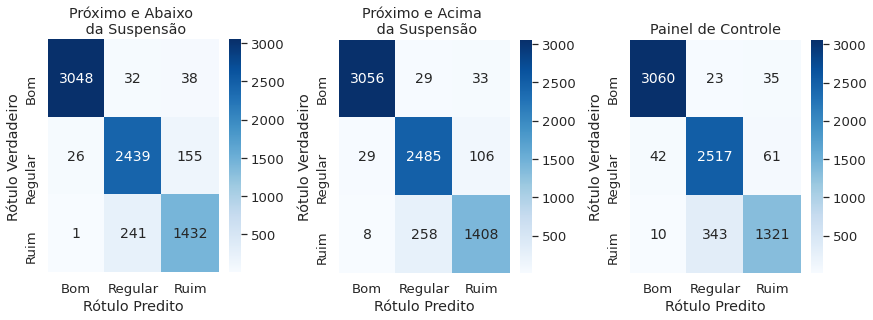
\includegraphics[width=1\textwidth]{figuras/fig_51.png}
  \fonte{Desenvolvido pelo autor.}
\end{figure}

Como podemos observar na \autoref{table:best_models_metrics_qualidade_superficie}, todas as classes de dados foram corretamente tratadas por todos os modelos sem haver viés, com valores acima de 80\%. Neste estudo, consideramos que o melhor modelo deve ser aquele que maximize tanto os VP quanto os VN, e minimize os FN e FP, de forma que a métrica \textit{f1-score} associa estes dois fatores. Analisando os valores, observamos que a rede CNN obteve os melhores resultados para praticamente todas as métricas em todas as classes, obtendo o melhor \textit{f1-score} em todas as classes. Sendo assim, consideramos o modelo baseado em CNN com janela de 500 amostras o melhor modelo para classificação de qualidade de superfície de pista, com valor de média entre \emph{experimentos por colocação} e \emph{experimentos por contexto} de 93,52\% para acurácia, 92,76\% para precisão, 91,52\% para \textit{recall} e 91,91\% para \textit{f1-score}. Na \autoref{fig:cnn_confusion_matrix_qualidade_superficie} é ilustrado a matriz confusão para o modelo baseado em CNN em cada ponto de coleta de dados.


\chapter{Reconhecimento de Lombadas}
\label{cap:deteccao_lombadas}

Nesta seção é apresentado o estudo voltado ao desenvolvimento de um modelo adaptativo para detecção de lombadas na via. Baseado nos experimentos das seções anteriores, este estudo focou no desenvolvimento de modelos baseados em \textit{Deep Learning}. Contudo, nos anteriores foi produzido modelos para classificação multi classe de eventos persistentes, enquanto neste os modelos consistem de uma classificação binária de evento transiente. O processo de desenvolvimento e experimentação é detalhado nas próximas subseções. Na primeira delas, o pré-processamento, foi realizada a seleção de variáveis, padronizado seus dados através de normalização dos sinais, e definido experimentos para avaliar aspectos como ponto de coleta de dados no veículo, tamanho da janela de dados e variações contextuais, onde foi possível analisar a capacidade de generalização do aprendizado dos modelos para contextos desconhecidos e, portanto, avaliar sua adaptabilidade. Na segunda subseção, processamento, foram desenvolvidos cinco modelos de DNN baseados em diferentes técnicas de \textit{Deep Learning}: LSTM, GRU, CNN, CNN-LSTM e ConvLSTM. Por fim, na última subseção são detalhados e comparados os resultados obtidos.

\section{Pré-Processamento}

Com base nos resultados obtidos nos experimentos das seções anteriores, neste estudo utilizamos como características de entrada os dados brutos das variáveis de aceleração em três eixos (X, Y, Z) e em três diferentes pontos de coleta (abaixo e próximo da suspensão, acima e próximo da suspensão e painel de controle), juntamente com os dados de taxa rotação em três eixos e em três diferentes pontos de coleta, além da velocidade do veículo. Inicialmente, todos os dados foram normalizados com \textit{Robust Scaler}, mantendo o sinal de direção do vetor de força. Após a normalização dos dados, para avaliar a influência da propriedade de dependência veicular e verificar a viabilidade de um modelo de classificação para os dados coletados em diferentes pontos do veículo, foram definidos os seguintes \emph{experimentos por colocação}, com base nos pontos de coleta de dados no veículo:

\begin{description}
	
	\item[Experimento por Colocação 1:] Foram utilizados os dados de força de aceleração 3D e taxa de rotação 3D amostrados próximo e abaixo da suspensão, mais a velocidade.
    
    \item[Experimento por Colocação 2:] Foram utilizados os dados de força de aceleração 3D e taxa de rotação 3D amostrados próximo e acima da suspensão, mais a velocidade.
    
    \item[Experimento por Colocação 3:] Foram utilizados os dados de força de aceleração 3D e taxa de rotação 3D amostrados no painel de controle, mais a velocidade.
    
\end{description}

Para avaliar a capacidade de generalização do aprendizado de cada técnica, avaliando sua adaptabilidade para contextos desconhecidos onde há variação nas propriedades de dependência veicular, de condução e ambiental, os dados de treinamento e validação foram divididos da mesma maneira que nos estudos das seções anteriores, separando-os de acordo com o conjunto de dados em três \emph{experimentos por contexto}:

\begin{description}
	
	\item[Experimento por Contexto 1:] O modelo aprende dados de todos os veículos e motoristas para alguns cenários; mas não todos os veículos com todos os motoristas para todos os cenários.
    \begin{itemize}
        \item \textbf{Treinamento (65\%):} PVS 1, PVS 3, PVS 4, PVS 6, PVS 7, PVS 9. 
        \item \textbf{Validação (35\%):} PVS 2, PVS 5, PVS 8.
    \end{itemize}
    
    \item[Experimento por Contexto 2:] O modelo aprende dados de todos os cenários para alguns veículos e alguns motoristas; mas não todos os veículos com todos os motoristas para todos os cenários.
    \begin{itemize}
        \item \textbf{Treinamento (66\%):} PVS 1, PVS 2, PVS 3, PVS 7, PVS 8, PVS 9.
        \item \textbf{Validação (34\%):} PVS 4, PVS 5, PVS 6.
    \end{itemize}
    
    \item[Experimento por Contexto 3:] O modelo aprende dados de alguns veículos com alguns motoristas para alguns cenários; mas não todos os veículos com todos os motoristas para todos os cenários.
    \begin{itemize}
        \item \textbf{Treinamento (66\%):} PVS 1, PVS 2, PVS 4, PVS 6, PVS 8, PVS 9.
        \item \textbf{Validação (34\%):} PVS 3, PVS 5, PVS 7.
    \end{itemize}
    
\end{description}

Neste estudo, para bem avaliar as variações contextuais, além de dados de lombadas em diferentes pavimentos, sendo asfalto e a paralelepípedo, os modelos ainda contam com amostras de vias de terra, as quais são importantes para os modelos minimizarem FP, uma vez que estradas de terra apresentam irregularidades que produzem assinaturas nos sinais semelhantes às produzidas por lombadas, sendo importante que os modelos saibam diferenciá-las. 

Finalmente, para analisar a influência do número de amostras na classificação, foram criados três \emph{experimentos por tamanho de janela de dados}, com janelas de 100, 200, 300, 400, e 500 amostras. A janela de dados utilizada foi deslizante com sobreposição total, e cada amostra correspondeu a um vetor com os valores das características. A aplicação de janela deslizante se mostra importante neste estudo para analisarmos o comportamento do modelo com entrada de dados em diferentes segmentos da lombada, como janelas com amostras do início, meio ou fim do obstáculo. Em resumo, cada experimento realizado neste estudo é um elemento do produto cartesiano entre \emph{experimentos por colocação}, \emph{experimentos por contexto} e \emph{experimentos por tamanho de janela de dados}.

Através da \autoref{table:lombada_metricas} observamos certo desbalanceamento das classes de dados. Sendo assim, se faz necessário analisar o grau desse desbalanceamento, uma vez que classes sub-representadas (\textit{minor data class}) podem não ser adequadamente tratadas pelos modelos, resultando em viés. Para avaliar a necessidade de aplicar técnicas de balanceamento, medimos a proporção de distribuição de cada classe de dados conforme detalhado \autoref{table:distribuicao_classes_lombadas}. A distribuição de classes foi calculada sobre os dados de treinamento, uma vez que são com estes que os modelos aprendem \cite{He2013, Kuhn2013}. A distribuição foi calculada em relação ao tamanho da janela de dados. Sendo assim, o valor detalhado em cada célula corresponde ao limite inferior e superior da distribuição da classe de dados, uma vez que cada tamanho da janela de dados apresenta uma pequena variação deste valor.

\begin{table}[h]
\caption{Distribuição de classes de lombadas}
\label{table:distribuicao_classes_lombadas}
\centering
\scriptsize
\begin{tabular}{lcccc}
\cmidrule(l){2-5}
\multicolumn{1}{c}{\multirow{2}{*}{\textbf{}}} & 
\multicolumn{4}{c}{\textbf{Classe de Dados}} \\ \cmidrule(l){2-5} 
\multicolumn{1}{c}{} & 
\multicolumn{2}{c}{\textbf{CL - Com Lombada}} & 
\multicolumn{2}{c}{\textbf{SL - Sem Lombada}} \\ \midrule
\textbf{Fonte de Dados} & 
\textit{\textbf{Percentual}} & 
\textit{\textbf{Proporção}} & 
\textit{\textbf{Percentual}} & 
\textit{\textbf{Proporção}} \\ \midrule
Exp. por Contexto 1 & 1.61\% - 1.45\% & 1:60.87 - 1:67.76 & 98.39\% - 98.55\% & 1:0.01 - 1:0.02 \\ \midrule
Exp. por Contexto 2 & 1.58\% - 1.36\% & 1:62.03 - 1:72.22 & 98.42\% - 98.64\% & 1:0.01 - 1:0.02 \\ \midrule
Exp. por Contexto 3 & 1.63\% - 1.44\% & 1:60.17 - 1:68.39 & 98.37\% - 98.56\% & 1:0.01 - 1:0.02 \\ \bottomrule
\end{tabular}
\fonte{Desenvolvido pelo autor.}
\end{table}

O desbalanceamento de classes pode ser considerado leve ou severo, onde as proporções de distribuição que variam de 1:4 até 1:100 (presença de 20\% - 1\%) são consideradas desbalanceamento leve e proporções de distribuição que variam de 1:100 ou mais (<1\% de presença) são consideradas desbalanceamentos severos \cite{Krawczyk2016,Brownlee2020}. Analisando a \autoref{table:distribuicao_classes_lombadas}, observamos que ambas as classes de dados apresentam desbalanceamentos leve, mas com alta tendência a desbalanceamentos severo. Para a classe \emph{Com Lombada (CL)}, a proporção varia entre 1:60.17 a 1:72.22, onde para 1 amostra da classe de dados \emph{CL}, há de 60.17 a 72.22 amostras da classe de dados \emph{Sem Lombada (SL)}. Portanto, realizamos \textit{downsampling} nos segmentos de dados sem lombada (\emph{SL}), descartando as janelas de sobreposição. Em suma, os dados onde há lombada contam com janela deslizante com sobreposição total, e onde não há lombada, a janela é fixa sem sobreposição. Com esta abordagem, a distribuição obtida é detalhada na \autoref{table:distribuicao_classes_lombadas_downsampling}, com uma redução da desproporção em aproximadamente 10 vezes.

\begin{table}[h]
\caption{Distribuição de classes de lombadas após \textit{downsampling}}
\label{table:distribuicao_classes_lombadas_downsampling}
\centering
\scriptsize
\begin{tabular}{lcccc}
\cmidrule(l){2-5}
\multicolumn{1}{c}{\multirow{2}{*}{\textbf{}}} & 
\multicolumn{4}{c}{\textbf{Classe de Dados}} \\ \cmidrule(l){2-5} 
\multicolumn{1}{c}{} & 
\multicolumn{2}{c}{\textbf{CL - Com Lombada}} & 
\multicolumn{2}{c}{\textbf{SL - Sem Lombada}} \\ \midrule
\textbf{Fonte de Dados} & 
\textit{\textbf{Percentual}} & 
\textit{\textbf{Proporção}} & 
\textit{\textbf{Percentual}} & 
\textit{\textbf{Proporção}} \\ \midrule
Exp. por Contexto 1 & 88.01\% - 62.12\% & 1:0.14 - 1:0.61 & 37.87\% - 11.99\% & 1:1.64 - 1:7.34 \\ \midrule
Exp. por Contexto 2 & 87.34\% - 61.68\% & 1:0.14 - 1:0.62 & 38.31\% - 12.66\% & 1:1.61 - 1:6.90 \\ \midrule
Exp. por Contexto 3 & 87.86\% - 62.41\% & 1:0.14 - 1:0.60 & 37.59\% - 12.14\% & 1:1.66 - 1:7.28 \\ \bottomrule
\end{tabular}
\fonte{Desenvolvido pelo autor.}
\end{table}

\section{Processamento}

Após o pré-processamento, os dados foram aplicados em cinco modelos de \textit{Deep Learning}, sendo baseados em LSTM, GRU, CNN, CNN-LSTM e ConvLSTM. Todos os modelos desenvolvidos são sequenciais e utilizam o otimizador Adam em conjunto com a função de perda Entropia Cruzada Binária. Todos os modelos tiveram seus hiperparâmetros ajustados (\textit{hyperparameter tuning}) utilizando o algoritmo \textit{HyperBand} implementado na biblioteca Keras Tuner, onde foram testados diferentes tipos de camadas, número de camadas e neurônios, funções de ativação e várias outras características para encontrar o conjunto ideal de hiper-parâmetros para cada DNN. 

O melhor modelo baseado em LSTM obtido através do ajuste de hiper-parâmetros é detalhado na \autoref{fig:best_lstm_tipo_lombadas}. O modelo DNN é composto de um bloco de camada de entrada, três blocos de camadas de recorrência e regularização e dois blocos de camada totalmente conectados para produção de saída. O bloco de entrada possui uma camada que recebe um tensor \emph{janelas x sequências x características}, onde \emph{janelas} são os agrupamentos de todas as janelas de dados, \emph{sequências} são as sequências de dados para cada janela, e \emph{características} são os valores das variáveis de entrada. Cada bloco de recorrência e regularização é composto por uma camada LSTM bidirecional de 128 unidades, seguida por uma camada de \textit{Batch Normalization} e uma camada de \textit{Dropout} em 25\%. Após o processamento nas camadas recorrentes, os parâmetros são passados para os blocos totalmente conectados, onde existem duas camadas \textit{Dense}, a primeira com 128 neurônios e ativação \textit{Relu}, e a segunda com 1 neurônio e ativação \textit{Sigmoid}. A saída produzida é uma resposta binária à presença ou ausência de lombadas na janela de dados. A saída esperada são os rótulos mais presentes na janela de dados.

\begin{figure}[h!]
  \centering
  \caption{Modelo LSTM para detecção de lombadas}
  \label{fig:best_lstm_tipo_lombadas}
  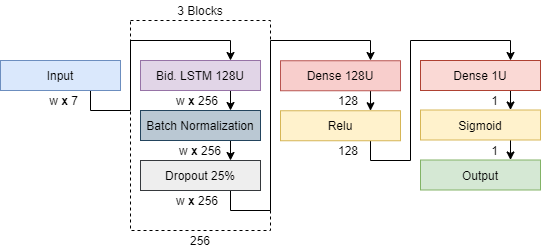
\includegraphics[width=0.75\textwidth]{figuras/fig_40.png}
 \fonte{Desenvolvido pelo autor.}
\end{figure}

O melhor modelo baseado em GRU obtido neste estudo está detalhado na \autoref{fig:best_gru_tipo_lombadas}. O modelo de DNN é composto de um bloco de camada de entrada, dois blocos de camadas de recorrência e regularização e dois blocos de camadas totalmente conectadas para produção de saída. O bloco de entrada possui uma camada que recebe um tensor \emph{janelas x sequências x características}, semelhante ao baseado em LSTM. Cada bloco de recorrência e regularização é composto por uma camada GRU bidirecional de 192 unidades, seguida por uma camada de \textit{Batch Normalization} e uma camada de \textit{Dropout} em 20\%. Após o processamento nas camadas recorrentes, os parâmetros passam para um bloco totalmente conectado, onde existem duas camadas \textit{Dense}, a primeira com 192 neurônios e ativação \textit{Relu}, e a segunda com 1 neurônio e ativação \textit{Sigmoid}, produzindo a resposta binária.

\begin{figure}[h!]
  \centering
  \caption{Modelo GRU para detecção de lombadas}
  \label{fig:best_gru_tipo_lombadas}
  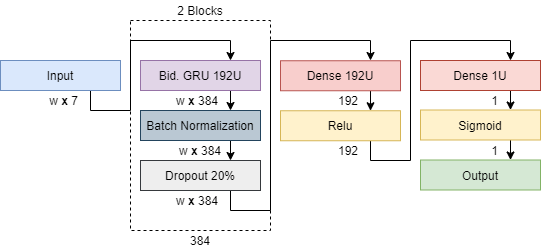
\includegraphics[width=0.75\textwidth]{figuras/fig_41.png}
 \fonte{Desenvolvido pelo autor.}
\end{figure}

O melhor modelo baseado em CNN obtido é detalhado na \autoref{fig:best_cnn_tipo_lombadas}. O modelo de DNN é composto de um bloco de entrada, dois blocos de convolução e regularização e dois blocos de camadas totalmente conectadas para produção de saída. O bloco de entrada possui uma camada que recebe um tensor \emph{janelas x sequências x características}, semelhante aos modelos baseados em LSTM e GRU. O primeiro bloco de convolução e regularização é composto por uma camada Conv 1D com 224 filtros com \textit{kernel} de tamanho 5 para extração de características e ativação \textit{Relu}, seguida de regularização através de uma camada de \textit{Batch Normalization} e uma camada de \textit{Spatial Dropout 1D} em 50\%. O último bloco de convolução e regularização tem uma camada Conv 1D com as mesmas configurações da anterior, uma camada \textit{Global Max Pooling 1D} para extrair recursos mais robustos por meio dos valores máximos em cada região, e camadas de regularização por \textit{Batch Normalization} e \textit{Dropout} em 50\%. Finalmente, os blocos totalmente conectados consistem em duas camadas \textit{Dense}, uma com 160 neurônios e ativação \textit{Relu} e outra com 1 neurônio e ativação \textit{Sigmoid}, produzindo a saída binária.

\begin{figure}[h!]
  \centering
  \caption{Modelo CNN para detecção de lombadas}
  \label{fig:best_cnn_tipo_lombadas}
  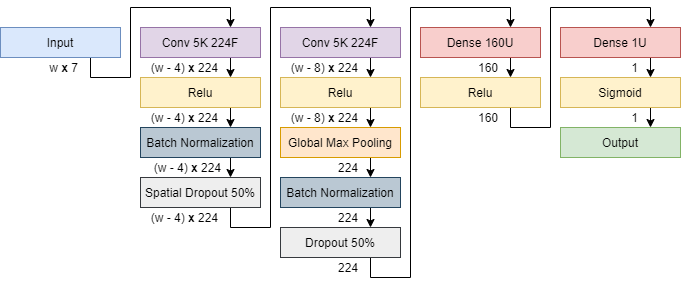
\includegraphics[width=0.9\textwidth]{figuras/fig_42.png}
 \fonte{Desenvolvido pelo autor.}
\end{figure}

\begin{figure}[h!]
  \centering
  \caption{Modelo CNN-LSTM para detecção de lombadas}
  \label{fig:best_cnn_lstm_tipo_lombadas}
  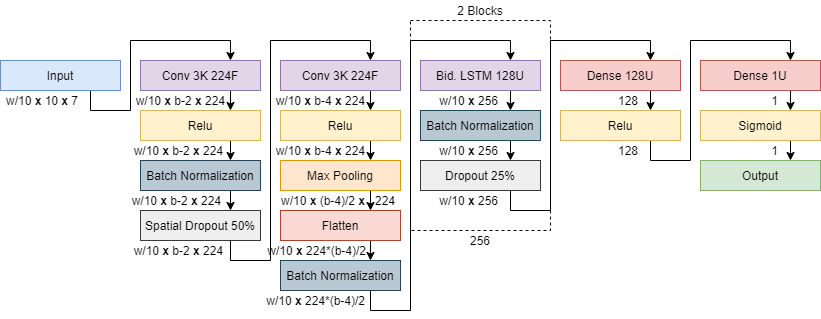
\includegraphics[width=1\textwidth]{figuras/fig_43.png}
 \fonte{Desenvolvido pelo autor.}
\end{figure}

O melhor modelo híbrido baseado em CNN-LSTM obtido é detalhado na \autoref{fig:best_cnn_lstm_tipo_lombadas}. O modelo de DNN baseado em CNN-LSTM desenvolvido é composto de um bloco de entrada, dois blocos de convolução e regularização, dois blocos recorrentes e de regularização e dois blocos de camada totalmente conectadas para produção de saída. O bloco de entrada tem uma camada que recebe um tensor \emph{janelas x sequências x subsequências x características}, onde \emph{janelas} são os agrupamentos de todas as janelas de dados, \emph{sequências} são as sequências de dados para cada janela, \emph{subsequências} são as subpartes da sequência de dados original, e \emph{características} os valores das variáveis de entrada. O primeiro bloco de convolução e regularização é composto por uma camada Conv 1D com 224 filtros com  \textit{kernel} de tamanho 3 para extração de características e ativação \textit{Relu}, seguida de regularização através de uma camada de \textit{Batch Normalization} e uma camada de \textit{Spatial Dropout 1D} em 50\%. O último bloco de convolução e regularização tem uma camada Conv 1D com as mesmas configurações da anterior, uma camada \textit{Max Pooling 1D} para extrair recursos mais robustos por meio dos valores máximos em cada região, uma camada \textit{Flatten} para reagrupar os recursos extraídos na sequência temporal original, e regularização por camada de \textit{Batch Normalization}. Em seguida, cada bloco de recorrência e regularização é composto por uma camada LSTM bidirecional de 128 unidades, seguida por uma camada de \textit{Batch Normalization} e uma camada de \textit{Dropout} em 25\%. Finalmente, os parâmetros resultantes passam para duas camadas \textit{Dense}, a primeira com 128 neurônios e ativação de \textit{Relu}, e a segunda com 1 neurônio e ativação de \textit{Sigmoid}, produzindo a saída binária. 

O melhor modelo baseado em ConvLSTM obtido é detalhado na Figura \autoref{fig:best_conv_lstm_tipo_lombadas}. O modelo DNN é composto de um bloco de entrada, dois blocos convolucionais recorrentes e de regularização, e dois blocos de camadas totalmente conectadas para produção de saída. O bloco de entrada possui uma camada que recebe um tensor \emph{janelas x sequências x subsequências x características}, semelhante ao modelo CNN-LSTM. Os dois blocos convolucionais recorrentes e de regularização são compostos por uma camada \textit{ConvLSTM 1D} com 224 filtros \textit{kernel} de tamanho 3 e ativação \textit{Relu}, seguido por regularização através de uma camada \textit{Dropout} em 30\%. Finalmente, os parâmetros resultantes são achatados (\textit{flattened)} e passados para duas camadas \textit{Dense}, a primeira com 224 neurônios e ativação \textit{Relu}, e a segunda com 1 neurônio e ativação \textit{Sigmoid}, produzindo a saída binária.

\begin{figure}[h!]
  \centering
  \caption{Modelo ConvLSTM para detecção de lombadas}
  \label{fig:best_conv_lstm_tipo_lombadas}
  \includegraphics[width=0.8\textwidth]{figuras/fig_44.png}
 \fonte{Desenvolvido pelo autor.}
\end{figure}

\section{Análise de Resultados}

Neste estudo todos os modelos de detecção de lombadas foram desenvolvidos na linguagem Python 3, utilizando da biblioteca Keras 2, a qual é uma API de alto nível do TensorFlow. Os hiperparâmetros dos modelos foram afinados através da biblioteca Keras Tuner. Todos os experimentos foram executados em máquinas do Google \textit{Collaboratory}, de mesma configuração dos estudos das seções anteriores. Cada experimento é um elemento do produto Cartesiano entre \emph{experimentos por colocação}, \emph{experimentos por contexto} e \emph{experimentos por tamanho da janela de dados}, sendo executado três vezes e recuperando-se o melhor das três execuções. Consideramos a melhor execução aquela com maior valor de acurácia na fase de validação, uma vez que o treinamento dos modelos foi configurado para maximizar a métrica de acurácia.

Os resultados obtidos com a execução de todos os experimentos são apresentados nas Tabelas \ref{table:lstm_accuracy_result_lombadas}-\ref{table:conv_lstm_accuracy_result_lombadas}. Em cada tabela são detalhados os resultados para determinado modelo de DNN, para cada colocação, contexto e janela de dados. Também são apresentadas métricas de média aritmética para cada tipo de experimento, sendo Acurácia Média dos Experimentos por Contexto (AMEC) e Acurácia Média dos Experimentos por Contexto e Colocação (AMECC), onde são destacados os menores e maiores valores de acurácia obtidos na fase de validação.

\begin{table}[H]
\scriptsize
\centering
\caption{Valores de acurácia em validação obtidos pelo modelo LSTM} 
\label{table:lstm_accuracy_result_lombadas}
\begin{tabular}{ccccccc}
\toprule
\multicolumn{2}{c}{\textbf{Tipo de Experimento}} & \multicolumn{5}{c}{\textit{\textbf{Tamanho da Janela de Dados}}} \\ \midrule
\textit{\textbf{Colocação}} & \textit{\textbf{Contexto}} & \textit{100} & \textit{200} & \textit{300} & \textit{400} & \textit{500} \\ \midrule
\multirow{4}{*}{\begin{tabular}[c]{@{}c@{}} \\ Próximo e Abaixo \\ da Suspensão\end{tabular}} 
& 1 & 95.03\% & 96.53\% & 98.59\% & 99.18\% & 99.21\% \\ \cmidrule(l){2-7} 
& 2 & 90.70\% & 94.33\% & 97.08\% & 97.12\% & 97.81\% \\ \cmidrule(l){2-7} 
& 3 & 95.05\% & 97.54\% & 98.66\% & 99.12\% & 98.52\% \\ \cmidrule(l){2-7} 
& AMEC & \cellcolor[HTML]{FFCCC9}93.59\% & 96.13\% & 98.11\% & 98.47\% & \cellcolor[HTML]{34FF34}98.52\% \\ \midrule
\multirow{4}{*}{\begin{tabular}[c]{@{}c@{}} \\ Próximo e Acima \\ da Suspensão\end{tabular}} 
& 1 & 92.77\% & 93.68\% & 97.83\% & 98.97\% & 98.46\% \\ \cmidrule{2-7} 
& 2 & 92.90\% & 94.98\% & 97.21\% & 97.76\% & 97.66\% \\ \cmidrule{2-7} 
& 3 & 95.00\% & 96.64\% & 98.60\% & 99.25\% & 99.30\% \\ \cmidrule{2-7} 
& AMEC & \cellcolor[HTML]{FFCCC9}93.56\% & 95.10\% & 97.88\% & \cellcolor[HTML]{34FF34}98.66\% & 98.47\%   \\ \midrule
\multirow{4}{*}{\begin{tabular}[c]{@{}c@{}} \\ Painel de Controle \end{tabular}} 
& 1 & 93.99\% & 94.55\% & 99.22\% & 98.77\% & 98.18\% \\ \cmidrule{2-7} 
& 2 & 92.10\% & 95.70\% & 97.37\% & 97.38\% & 98.48\% \\ \cmidrule{2-7} 
& 3 & 95.19\% & 97.36\% & 99.24\% & 99.33\% & 98.62\% \\ \cmidrule{2-7} 
& AMEC & \cellcolor[HTML]{FFCCC9}93.76\% & 95.87\% & \cellcolor[HTML]{34FF34}98.61\% & 98.49\% & 98.43\%  \\ \midrule
& AMECC & \cellcolor[HTML]{FFCCC9}93.64\% & 95.70\% & 98.20\% & \cellcolor[HTML]{34FF34}98.54\% & 98.47\% \\ \cmidrule(l){2-7} 
\end{tabular}
\fonte{Desenvolvido pelo autor.}
\end{table}

\begin{table}[H]
\scriptsize
\centering
\caption{Valores de acurácia em validação obtidos pelo modelo GRU} 
\label{table:gru_accuracy_result_lombadas}
\begin{tabular}{ccccccc}
\toprule
\multicolumn{2}{c}{\textbf{Tipo de Experimento}} & \multicolumn{5}{c}{\textit{\textbf{Tamanho da Janela de Dados}}} \\ \midrule
\textit{\textbf{Colocação}} & \textit{\textbf{Contexto}} & \textit{100} & \textit{200} & \textit{300} & \textit{400} & \textit{500} \\ \midrule
\multirow{4}{*}{\begin{tabular}[c]{@{}c@{}} \\ Próximo e Abaixo \\ da Suspensão\end{tabular}} 
 & 1 & 94.23\% & 96.42\% & 97.84\% & 98.60\% & 95.78\% \\ \cmidrule{2-7} 
 & 2 & 92.76\% & 94.20\% & 96.83\% & 96.54\% & 97.25\% \\ \cmidrule{2-7} 
 & 3 & 94.46\% & 97.54\% & 98.55\% & 98.88\% & 96.17\% \\ \cmidrule{2-7} 
 & AMEC & \cellcolor[HTML]{FFCCC9}93.82\% & 96.05\% & 97.74\% & \cellcolor[HTML]{34FF34}98.01\% & 96.40\% \\ \midrule
\multirow{4}{*}{\begin{tabular}[c]{@{}c@{}} \\ Próximo e Acima \\ da Suspensão\end{tabular}} 
 & 1 & 93.57\% & 93.61\% & 98.23\% & 94.44\% & 95.45\% \\ \cmidrule{2-7} 
 & 2 & 90.93\% & 94.17\% & 97.17\% & 97.39\% & 96.45\% \\ \cmidrule{2-7} 
 & 3 & 93.90\% & 96.82\% & 98.53\% & 98.00\% & 98.62\% \\ \cmidrule{2-7} 
 & AMEC & \cellcolor[HTML]{FFCCC9}92.80\% & 94.87\% & \cellcolor[HTML]{34FF34}97.98\% & 96.61\% & 96.84\% \\ \midrule
\multirow{4}{*}{\begin{tabular}[c]{@{}c@{}} \\ Painel de Controle \end{tabular}} 
 & 1 & 94.41\% & 96.78\% & 97.94\% & 96.88\% & 95.92\% \\ \cmidrule{2-7} 
 & 2 & 92.05\% & 96.37\% & 96.91\% & 98.05\% & 93.01\% \\ \cmidrule{2-7} 
 & 3 & 94.64\% & 96.93\% & 98.54\% & 99.18\% & 97.38\% \\ \cmidrule{2-7} 
 & AMEC & \cellcolor[HTML]{FFCCC9}93.70\% & 96.69\% & 97.80\% & \cellcolor[HTML]{34FF34}98.04\% & 95.44\% \\ \midrule
& AMECC  & \cellcolor[HTML]{FFCCC9}93.44\% & 95.87\% & \cellcolor[HTML]{34FF34}97.84\% & 97.55\% & 96.23\% \\ \cmidrule(l){2-7} 
\end{tabular}
\fonte{Desenvolvido pelo autor.}
\end{table}

\begin{table}[H]
\scriptsize
\centering
\caption{Valores de acurácia em validação obtidos pelo modelo CNN} 
\label{table:cnn_accuracy_result_lombadas}
\begin{tabular}{ccccccc}
\toprule
\multicolumn{2}{c}{\textbf{Tipo de Experimento}} & \multicolumn{5}{c}{\textit{\textbf{Tamanho da Janela de Dados}}} \\ \midrule
\textit{\textbf{Colocação}} & \textit{\textbf{Contexto}} & \textit{100} & \textit{200} & \textit{300} & \textit{400} & \textit{500} \\ \midrule
\multirow{4}{*}{\begin{tabular}[c]{@{}c@{}} \\ Próximo e Abaixo \\ da Suspensão\end{tabular}} 
 & 1 & 94.20\% & 95.12\% & 97.38\% & 97.45\% & 99.8\% \\ \cmidrule{2-7} 
 & 2 & 91.02\% & 90.57\% & 93.32\% & 95.33\% & 95.73\% \\ \cmidrule{2-7} 
 & 3 & 95.55\% & 96.07\% & 97.62\% & 98.32\% & 99.36\% \\ \cmidrule{2-7} 
 & AMEC & \cellcolor[HTML]{FFCCC9}93.59\% & 93.92\% & 96.11\% & 97.03\% & \cellcolor[HTML]{34FF34}98.30\% \\ \midrule
\multirow{4}{*}{\begin{tabular}[c]{@{}c@{}} \\ Próximo e Acima \\ da Suspensão\end{tabular}} 
 & 1 & 95.1\% & 96.08\% & 97.18\% & 97.55\% & 98.85\% \\ \cmidrule{2-7} 
 & 2 & 93.77\% & 94.40\% & 96.96\% & 97.66\% & 97.11\% \\ \cmidrule{2-7} 
 & 3 & 95.11\% & 95.94\% & 98.67\% & 99.40\% & 97.84\% \\ \cmidrule{2-7} 
 & AMEC & \cellcolor[HTML]{FFCCC9}94.66\% & 95.48\% & 97.60\% & \cellcolor[HTML]{34FF34}98.20\% & 97.93\% \\ \midrule
\multirow{4}{*}{\begin{tabular}[c]{@{}c@{}} \\ Painel de Controle \end{tabular}} 
 & 1 & 95.41\% & 95.69\% & 97.61\% & 97.84\% & 99.78\% \\ \cmidrule{2-7} 
 & 2 & 94.43\% & 93.59\% & 96.24\% & 97.19\% & 97.41\% \\ \cmidrule{2-7} 
 & 3 & 95.57\% & 95.11\% & 97.51\% & 98.52\% & 98.96\% \\ \cmidrule{2-7} 
 & AMEC & 95.14\% & \cellcolor[HTML]{FFCCC9}94.80\% & 97.12\% & 97.85\% & \cellcolor[HTML]{34FF34}98.72\% \\ \midrule
 & AMECC & \cellcolor[HTML]{FFCCC9}94.46\% & 94.73\% & 96.94\% & 97.69\% & \cellcolor[HTML]{34FF34}98.32\% \\ \cmidrule(l){2-7} 
\end{tabular}
\fonte{Desenvolvido pelo autor.}
\end{table}

\begin{table}[H]
\scriptsize
\centering
\caption{Valores de acurácia em validação obtidos pelo modelo CNN-LSTM} 
\label{table:cnn_lstm_accuracy_result_lombadas}
\begin{tabular}{ccccccc}
\toprule
\multicolumn{2}{c}{\textbf{Tipo de Experimento}} & \multicolumn{5}{c}{\textit{\textbf{Tamanho da Janela de Dados}}} \\ \midrule
\textit{\textbf{Colocação}} & \textit{\textbf{Contexto}} & \textit{100} & \textit{200} & \textit{300} & \textit{400} & \textit{500} \\ \midrule
\multirow{4}{*}{\begin{tabular}[c]{@{}c@{}} \\ Próximo e Abaixo \\ da Suspensão\end{tabular}} 
 & 1 & 94.49\% & 96.76\% & 98.95\% & 99.08\% & 98.20\% \\ \cmidrule{2-7} 
 & 2 & 94.30\% & 94.63\% & 96.83\% & 97.72\% & 96.79\% \\ \cmidrule{2-7} 
 & 3 & 95.13\% & 97.75\% & 98.89\% & 98.92\% & 98.93\% \\ \cmidrule{2-7} 
 & AMEC & \cellcolor[HTML]{FFCCC9}94.64\% & 96.38\% & 98.22\% & \cellcolor[HTML]{34FF34}98.57\% & 97.97\% \\ \midrule
\multirow{4}{*}{\begin{tabular}[c]{@{}c@{}} \\ Próximo e Acima \\ da Suspensão\end{tabular}} 
 & 1 & 94.14\% & 96.63\% & 98.75\% & 99.25\% & 99.79\% \\ \cmidrule{2-7} 
 & 2 & 92.78\% & 94.99\% & 97.33\% & 97.39\% & 97.67\% \\ \cmidrule{2-7} 
 & 3 & 94.92\% & 96.77\% & 99.21\% & 99.11\% & 99.38\% \\ \cmidrule{2-7} 
 & AMEC & \cellcolor[HTML]{FFCCC9}93.95\% & 96.13\% & 98.43\% & 98.59\% & \cellcolor[HTML]{34FF34}98.94\% \\ \midrule
\multirow{4}{*}{\begin{tabular}[c]{@{}c@{}} \\ Painel de Controle \end{tabular}} 
 & 1 & 94.18\% & 96.46\% & 99.1\% & 99.22\% & 99.73\% \\ \cmidrule{2-7} 
 & 2 & 92.74\% & 96.2\% & 97.37\% & 97.44\% & 97.46\% \\ \cmidrule{2-7} 
 & 3 & 94.86\% & 96.89\% & 99.13\% & 98.76\% & 99.41\% \\ \cmidrule{2-7} 
 & AMEC & \cellcolor[HTML]{FFCCC9}93.93\% & 96.52\% & 98.53\% & 98.48\% & \cellcolor[HTML]{34FF34}98.87\% \\ \midrule
 & AMECC & \cellcolor[HTML]{FFCCC9}94.17\% & 96.34\% & 98.39\% & 98.55\% & \cellcolor[HTML]{34FF34}98.59\% \\ \cmidrule(l){2-7} 
\end{tabular}
\fonte{Desenvolvido pelo autor.}
\end{table}

\begin{table}[H]
\scriptsize
\centering
\caption{Valores de acurácia em validação obtidos pelo modelo ConvLSTM} 
\label{table:conv_lstm_accuracy_result_lombadas}
\begin{tabular}{ccccccc}
\toprule
\multicolumn{2}{c}{\textbf{Tipo de Experimento}} & \multicolumn{5}{c}{\textit{\textbf{Tamanho da Janela de Dados}}} \\ \midrule
\textit{\textbf{Colocação}} & \textit{\textbf{Contexto}} & \textit{100} & \textit{200} & \textit{300} & \textit{400} & \textit{500} \\ \midrule
\multirow{4}{*}{\begin{tabular}[c]{@{}c@{}} \\ Próximo e Abaixo \\ da Suspensão\end{tabular}} 
 & 1 & 93.77\% & 96.21\% & 97.91\% & 98.43\% & 98.30\% \\ \cmidrule{2-7} 
 & 2 & 91.57\% & 94.92\% & 97.19\% & 96.22\% & 95.93\% \\ \cmidrule{2-7} 
 & 3 & 94.82\% & 96.73\% & 98.57\% & 98.74\% & 97.12\% \\ \cmidrule{2-7} 
 & AMEC & \cellcolor[HTML]{FFCCC9}93.39\% & 95.95\% & \cellcolor[HTML]{34FF34}97.89\% & 97.79\% & 97.12\% \\ \midrule
\multirow{4}{*}{\begin{tabular}[c]{@{}c@{}} \\ Próximo e Acima \\ da Suspensão\end{tabular}} 
 & 1 & 92.92\% & 96.12\% & 97.86\% & 98.21\% & 98.95\% \\ \cmidrule{2-7} 
 & 2 & 92.72\% & 96.60\% & 97.65\% & 96.93\% & 97.52\% \\ \cmidrule{2-7} 
 & 3 & 94.24\% & 96.39\% & 98.48\% & 99.30\% & 99.17\% \\ \cmidrule{2-7} 
 & AMEC & \cellcolor[HTML]{FFCCC9}93.29\% & 96.37\% & 98.00\% & 98.15\% & \cellcolor[HTML]{34FF34}98.55\% \\ \midrule
\multirow{4}{*}{\begin{tabular}[c]{@{}c@{}} \\ Painel de Controle \end{tabular}} 
 & 1 & 94.95\% & 96.68\% & 98.41\% & 99.28\% & 98.79\% \\ \cmidrule{2-7} 
 & 2 & 93.25\% & 95.90\% & 97.31\% & 98.92\% & 98.36\% \\ \cmidrule{2-7} 
 & 3 & 95.04\% & 97.36\% & 98.77\% & 99.35\% & 99.66\% \\ \cmidrule{2-7} 
 & AMEC & \cellcolor[HTML]{FFCCC9}94.41\% & 96.65\% & 98.16\% & \cellcolor[HTML]{34FF34}99.18\% & 98.94\% \\ \midrule
 & AMECC & \cellcolor[HTML]{FFCCC9}93.70\% & 96.32\% & 98.02\% & \cellcolor[HTML]{34FF34}98.37\% & 98.20\% \\ \cmidrule(l){2-7} 
\end{tabular}
\fonte{Desenvolvido pelo autor.}
\end{table}

Em nossa análise, para avaliar a habilidade dos modelos generalizarem seu aprendizado para contextos desconhecidos, como diferentes veículos, motoristas ou ambientes, consideramos que o modelo deve obter bom desempenho nos três \emph{experimentos por contexto}. Sendo assim, nossa análise é pautada inicialmente na média de acurácia destes experimentos, representada pela métrica AMEC. Através dos valores AMEC detalhados nas Tabelas \ref{table:lstm_accuracy_result_lombadas}-\ref{table:conv_lstm_accuracy_result_lombadas}, observamos que todos os modelos de DNN desenvolvidos obtiveram bons resultados independentes do contexto, com o valor de média de acurácia variando entre 92.80\% e 99.18\% conforme modelo e ponto de coleta de dados.

Analisando o impacto do tamanho das janelas de dados, observamos que as janelas de 100 e 200 amostras obtiveram todos os piores resultados para todos os experimentos e modelos, denotando ser uma quantidade de amostras insuficientes para reconhecer lombadas com uma boa confiabilidade. Nestas duas janelas estão as maiores variações dos valores de acurácia, onde a janela de dados de 100 amostras obteve acurácia média de 93.70\%, e a de 200 amostras obteve 95.87\%. Por outro lado, as janelas de 300, 400 e 500 amostras obtiveram os melhores resultados, com uma estabilização dos valores de acurácia, apresentando uma variação muito pequena. Na média entre todos os experimentos e modelos, a janela de 300 amostras obteve acurácia de 98.02\%, a de 400 obteve 98.37\%, e a de 500 obteve 98.32\%. Neste estudo, uma lombada inteira possuí entre 223 a 419 amostras. Logo, podemos concluir que os modelos necessitam de que a janela de dados contenha a lombada por inteiro o muito próximo disso para obter melhores resultados.

Em relação aos pontos de coleta de dados, todos obtiveram bons resultados, com pequena variação de uma colocação para outra. Os valores de média acurácia AMEC entre os modelos para a colocação próximo e abaixo da suspensão variaram de 93.39\% até 98.57\%; para próximo e acima da suspensão de 92.80\% até 98.94\%; e no painel de controle de 93.70\% até 99.18\%. A escolha do melhor modelo neste ponto pode levar em consideração a aplicação final, onde o modelo baseado em CNN-LSTM se mostra melhor para quando os sensores são empregados próximo e abaixo da suspensão ou próximo e acima da suspensão, enquanto que o modelo baseado em ConvLSTM se mostra melhor para aplicação no painel de controle. Contudo, neste estudo consideramos que o melhor modelo deve possibilitar sua operação independentemente do local de colocação dos sensores no veículo. Portanto, deve ser aquele com melhor desempenho entre os diferentes pontos de coleta, representado pela média de acurácia entre os \emph{experimentos por colocação}. Sendo assim, esta métrica é detalhada nas tabelas por AMECC, onde para determinar a melhor configuração de janela para cada modelo é considerado a média de acurácia entre todos os \emph{experimentos por colocação} e \emph{experimentos por contexto}.

Através da métrica supracitada, observamos que o melhor modelo é o baseado em CNN-LSTM em janela de 500 amostras, resultando em média de acurácia de 98.59\%. O segundo melhor é o baseado em LSTM com 400 amostras resultando em 98.54\%. O terceiro o baseado em ConvLSTM de 400 amostras com 98.37\%. Em quarto o baseado em CNN de 500 amostras com 98.32\%. Por último, o modelo baseado em GRU de 300 amostras resultando em 97.84\%. A melhor configuração de cada modelo é detalhada na Tabela \ref{table:best_models_metrics_lombadas} com as demais métricas de avaliação. Todos os valores das métricas apresentadas nesta tabela correspondem a média entre os \emph{experimentos por colocação} e \emph{experimentos por contexto}.

\begin{table}[H]
\scriptsize
\centering
\caption{Métricas de avaliação para a melhor configuração de cada modelo DNN} 
\label{table:best_models_metrics_lombadas}
\begin{tabular}{ccccccc}
\toprule
\multirow{2}{*}{\textbf{\begin{tabular}[c]{@{}c@{}}Métrica de \\ Avaliação\end{tabular}}} & \textbf{Modelo} & LSTM & GRU & CNN & CNN-LSTM & ConvLSTM \\ \cmidrule(l){2-7} 
 & \textbf{Janela} & 400 & 300 & 500 & 500 & 400 \\ \midrule
\multirow{2}{*}{Acurácia} 
 & Treinamento & 99.21\% & 99.71\% & 99.11\% & 99.53\% & 99.56\% \\ \cmidrule{2-7} 
 & Validação & 98.54\% & 97.84\% & 98.32\% & \cellcolor[HTML]{34FF34}98.59\% & 98.37\%  \\ \midrule
\multirow{3}{*}{\begin{tabular}[c]{@{}c@{}} \\ Precisão\end{tabular}} 
 & CL & 99.25\% & 99.64\% & \cellcolor[HTML]{34FF34}99.67\% & 99.64\% & 99.22\% \\ \cmidrule{2-7} 
 & SL & \cellcolor[HTML]{34FF34}94.40\% & 90.40\% & 90.57\% & 92.34\% & 93.49\% \\ \cmidrule{2-7} 
 & Média & \cellcolor[HTML]{34FF34}96.83\% & 95.02\% & 95.12\% & 95.99\% & 96.36\% \\ \midrule
\multirow{3}{*}{\begin{tabular}[c]{@{}c@{}} \\ Recall\end{tabular}} 
 & CL & \cellcolor[HTML]{34FF34}99.06\% & 97.73\% & 98.40\% & 98.75\% & 98.89\% \\ \cmidrule{2-7} 
 & SL & 95.32\% & \cellcolor[HTML]{34FF34}98.36\% & 97.83\% & 97.59\% & 95.13\% \\ \cmidrule{2-7} 
 & Média & 97.19\% & 98.05\% & 98.12\% & \cellcolor[HTML]{34FF34}98.17\% & 97.01\% \\ \midrule
\multirow{3}{*}{\begin{tabular}[c]{@{}c@{}} \\ F1-Score\end{tabular}} 
 & CL & 99.15\% & 98.67\% & 99.02\% & \cellcolor[HTML]{34FF34}99.19\% & 99.05\% \\ \cmidrule{2-7} 
 & SL & \cellcolor[HTML]{34FF34}94.77\% & 94.18\% & 93.83\% & 94.74\% & 94.18\% \\ \cmidrule{2-7} 
 & Média & 96.96\% & 96.43\% & 96.43\% & \cellcolor[HTML]{34FF34}96.97\% & 96.62\%  \\ \bottomrule
\end{tabular}
\fonte{Desenvolvido pelo autor.}
\end{table}

Na \autoref{table:best_models_metrics_lombadas} são apresentadas as métricas de acurácia, precisão, \textit{recall} e \textit{f1-score} para cada melhor configuração dos modelos. Embora a acurácia seja amplamente utilizada, em conjuntos de dados com desbalanceamento ela pode esconder viés, especialmente quando a classe minoritária não é bem tratada pelo modelo \cite{He2013}. Para isto são utilizadas as métricas de avaliação precisão, \textit{recall} e \textit{f1-score}, analisando a performance do modelo em cada classe de dados. Na tabela, para cada métrica são apresentadas os valores para as duas classes de dados deste estudo: \emph{Com Lombada} (CL) e \emph{Sem Lombada} (SL). Como podemos observar, todas as classes de dados foram corretamente tratadas por todos os modelos sem haver viés, de forma que a técnica de \textit{downsampling} empregada foi efetiva. Todas as métricas obtiveram valores acima de 90\%. Neste estudo, consideramos que o melhor modelo deve ser aquele que maximize tanto os VP quanto os VN, e minimize os FN e FP. Desta forma, o modelo deve ter a melhor performance tanto na detecção correta de lombadas quanto a detecção correta de não lombadas. Sendo assim, a métrica de \textit{f1-score} associa estes dois fatores, e na média para as duas classes de dados o modelo baseado em CNN-LSTM com janela de 500 amostras foi o que obteve melhor resultado. Portanto, consideramos o modelo baseado em CNN-LSTM o melhor modelo para detecção de lombadas, com valor de média entre \emph{experimentos por colocação} e \emph{experimentos por contexto} de 98.59\% para acurácia, 95.99\% para precisão, 98.17\% para \textit{recall} e 96.97\% para \textit{f1-score}. Na \autoref{fig:cnn_lstm_confusion_matrix_lombadas} é ilustrado a matriz confusão para o modelo baseado em CNN-LSTM em cada ponto de coleta de dados.

\begin{figure}[H]
  \centering
  \caption{Matriz de confusão para o modelo CNN-LSTM em cada ponto de coleta de dados}
  \label{fig:cnn_lstm_confusion_matrix_lombadas}
  \includegraphics[width=1\textwidth]{figuras/fig_45.png}
  \fonte{Desenvolvido pelo autor.}
\end{figure}


\chapter{Materiais Resultantes}
\label{cap:materiais_resultantes}

A realização deste trabalho resultou em diverso materiais disponíveis publicamente na página do projeto no Github \footnote{https://github.com/Intelligent-Vehicle-Perception/Intelligent-Vehicle-Perception-Based-on-Inertial-Sensing-and-Artificial-Intelligence} \footnote{https://codigos.ufsc.br/lapix/intelligent-vehicle-perception-based-on-inertial-sensing}. Os seguintes materiais de \textit{software} foram produzidos:

\begin{small}
\begin{description}
	
	\item[Módulo de Coleta de Dados e Pré-Processamento:] contém o código-fonte dos projetos utilizados para coleta e ajuste dos dados, tal como gerenciamento de sensores para amostragem, armazenamento dos sinais, sincronização de sensores multimodais, fusão de dados, criação de GT, visualização de dados brutos, criação de vídeos integrando dados de MPU, GPS e câmera, etc.
	
	\item[Módulo de Conjuntos de Dados:] contém todos os conjuntos de dados PVS produzidos.
	
    \item[Módulo de Classificação de Tipo de Superfície de Pista 1:] código-fonte com todos os modelos desenvolvidos para o primeiro estudo de classificação de tipo de superfície, juntamente com todos os experimentos executados, permitindo pesquisas futuras executarem, compararem e auditarem.
    
    \item[Módulo de Classificação de Tipo de Superfície de Pista 2:] código-fonte com todos os modelos desenvolvidos para o segundo estudo de classificação de tipo de superfície, juntamente com todos os experimentos executados, permitindo pesquisas futuras executarem, compararem e auditarem.
    
    \item[Módulo de Classificação de Qualidade de Superfície de Pista:] código-fonte com todos os modelos desenvolvidos para o estudo de classificação de qualidade de superfície, juntamente com todos os experimentos executados, permitindo pesquisas futuras executarem, compararem e auditarem.
    
    \item[Módulo de Reconhecimento de Lombadas:] código-fonte com todos os modelos desenvolvidos para o estudo de detecção de lombadas, juntamente com todos os experimentos executados, permitindo pesquisas futuras executarem, compararem e auditarem.
    
    \item[Módulo de Melhores Modelos de Percepção Veicular:] código-fonte simplificado para uso dos melhores modelos desenvolvidos, sendo eles:
    \begin{itemize}
        \item Classificação de Tipo de Superfície de Pista: modelo CNN, classificando em terra, paralelepípedo e asfalto.
        \item Classificação de Qualidade de Superfície de Pista: modelo CNN, classificando em bom, regular e ruim.
        \item Reconhecimento de Lombadas: modelo CNN-LSTM, detectando lombadas.
    \end{itemize}

\end{description}
\end{small}

Todos os módulos descritos compõe o programa \textit{Intelligent Road Assessment System} (IRAS), o qual já possuí Registro do Programa de Computador no Instituto Nacional da Propriedade Industrial (INPI), sendo distriuído sob a licença \textbf{CC BY-NC-ND 4.0}. Em relação ao \textit{hardware} e rede de sensores desenvolvida, pedido de patente e/ou modelo de utilidade estão sendo analisados. Para promover a pesquisa e auxiliar na popularização deste tipo de sensoriamento em ITS, foi criado um canal no Youtube \footnote{https://www.youtube.com/channel/UCoWKXjgUNhGCYieR-ys-IBw}, com divulgação de apresentações, vídeos didáticos e vídeos com os melhores modelos em execução produzindo seus reconhecimentos e classificações. Também estão em produção artigos acessíveis para público não especializado, que serão publicados no \textit{Medium} e \textit{Towards Data Science}. Em relação às publicações científicas, foram produzidos os seguintes artigos: 

\begin{small}
\begin{description}

    \item \textbf{\textit{\href{http://www.incod.ufsc.br/wp-content/uploads/2018/10/INCoD-TR-2018-07-LAPIX-E-V01.pdf}{Vehicular Perception and Proprioception Based on Inertial Sensing: a Systematic Review}}} \phantom{ } 
    \newline\textbf{Editora}: \textit{Brazilian National Institute for Digital Convergence}. 
    \newline\textbf{Status}: Publicado.
    \newline\textbf{Ano}: 2018.
    \newline\textbf{Qualis}: C.

    \item \textbf{\href{https://siaiap32.univali.br/seer/index.php/acotb/article/view/14375}{Classificação de Qualidade de Superfície de Pista Baseado em Sensoriamento Inercial e Lógica \textit{Fuzzy}}} \phantom{ } 
    \newline\textbf{Editora}: UNIVALI. Anais do \textit{Computer on the Beach}. 
    \newline\textbf{Status}: Publicado.
    \newline\textbf{Ano}: 2019.
    \newline\textbf{Qualis}: B4.
    
    \item \textbf{\textit{\href{https://link.springer.com/article/10.1007\%2Fs42979-020-00275-z}{Vehicular Perception Based on Inertial Sensing - A Structured Mapping of Approaches and Methods}}}\phantom{ } 
    \newline\textbf{Editora}: Springer. Revista \textit{SN Computer Science}. 
    \newline\textbf{Status}: Publicado.
    \newline\textbf{Ano}: 2020.
    \newline\textbf{Qualis}: Indefinido.
    
    \item \textbf{\textit{\href{https://ieeexplore.ieee.org/document/9277846}{Multi-Contextual and Multi-Aspect Analysis for Road Surface Type Classification Through Inertial Sensors and Deep Learning}}} \phantom{ } 
    \newline\textbf{Editora}: IEEE Xplore. Anais do \textit{2020 X Brazilian Symposium on Computing Systems Engineering} (SBESC). 
    \newline\textbf{Status}: Publicado.
    \newline\textbf{Ano}: 2020.
    \newline\textbf{Qualis}: B2.
    
    \item \textbf{\textit{\href{https://link.springer.com/article/10.1007/s00607-021-00914-0}{Road Surface Type Classification Based on Inertial Sensors and Machine Learning: A Comparison Between Classical and Deep Machine Learning Approaches For Multi-Contextual Real-world Scenarios}}} \phantom{ } 
    \newline\textbf{Editora}: Springer. Revista \textit{Computing}.  
    \newline\textbf{Status}: Publicado.
    \newline\textbf{Ano}: 2021.
    \newline\textbf{Qualis}: B1.
    
    \item \textbf{\textit{\href{}{Speed Bump Detection Through Inertial Sensors and Deep Learning in a Multi-Contextual Analysis}}}\phantom{ } 
    \newline\textbf{Editora}: Springer. Revista \textit{Neural Processing Letters}.  
    \newline\textbf{Status}: Em Revisão.
    \newline\textbf{Ano}: 2021.
    \newline\textbf{Qualis}: A2.

\end{description}
\end{small}

%%%%%%%%%%%%%%%%%%%%%%%%%%%%%%%%%%%%%%%%%%%%%%%%%%%%%%%%%%%%%%%%%%%%
%%% Elementos pós-textuais                                       %%%
%%%%%%%%%%%%%%%%%%%%%%%%%%%%%%%%%%%%%%%%%%%%%%%%%%%%%%%%%%%%%%%%%%%%

\postextual
\bibliography{bibliografia}

\end{document}

% LocalWords:  pdf ufsc-thesis-rn abntex PPGCC Zambonin pull request GitHub PRs
% LocalWords:  alexishuf Issues alpha drop-in template cls shell-escape ZIP Git
% LocalWords:  UNIX-like Makefile git submodule shame on you Overleaf english
% LocalWords:  overview Pós-Graduação Prof BU pdfpages bug BibTeX URLs at bst
% LocalWords:  Available cite-alf url x-url brazil embeddedlogo auto-contido pt
% LocalWords:  lmodern arial open-source Latin Modern nocapautoref ufsc-thesis
% LocalWords:  working directory pdflatex tex dijkstra diffie Saleem Ullman rdf
% LocalWords:  magic Distefano Abiteboul Forgy default Word captions userguide
% LocalWords:  noplainurl noabntexcite begin dedicatoria end doc abstracts EQM
% LocalWords:  corretude indentação oneside memoir feature SAD EQD bookmarks of
% LocalWords:  nopretextualbookmark listoffigures table contents
